\documentclass[12pt]{article}

\usepackage[utf8]{inputenc}
\usepackage[T1]{fontenc}
\usepackage{lmodern}
\usepackage[margin=1in]{geometry}
\usepackage{amsmath,amssymb,bm}
\usepackage{graphicx}
\usepackage{booktabs}
\usepackage{multirow}
\usepackage{array}
\usepackage{xcolor}
\usepackage{tikz}
\usetikzlibrary{arrows.meta,decorations.pathreplacing,calc}
\usepackage[font=small,labelfont=bf]{caption}
\usepackage{enumitem}
\usepackage{authblk}
\usepackage{lineno}
\usepackage{abstract}
\usepackage[round,authoryear]{natbib}
\usepackage[colorlinks=true,linkcolor=blue!60!black,citecolor=blue!60!black,urlcolor=blue!60!black]{hyperref}
\usepackage{microtype}
\usepackage[section]{placeins}

\graphicspath{{../figures/}}

% notes to self
\newcommand{\anote}[1]{\textcolor{red}{[#1]}}

% notation
\newcommand{\prgh}{p_{\mathrm{rgh}}}
\newcommand{\dd}{\mathrm{d}}
\newcommand{\code}[1]{\texttt{#1}}
\newcommand{\NHFOAM}{NHFOAM}

\setlength{\parskip}{0.4em}

\title{NHFOAM: a non-hydrostatic $\sigma$-layer wave model in OpenFOAM\\[0.4em]
\large Model description, verification, and validation against NHWAVE,\\ with wetting and drying, breaking, longshore currents and wave input}

\author[1]{Mohammadsadegh Nouri\thanks{Corresponding author: \href{mailto:msnouri@udel.edu}{msnouri@udel.edu}}}
\affil[1]{Center for Applied Coastal Research, Department of Civil, Construction, and Environmental Engineering, University of Delaware, Newark, DE 19716, USA}
\date{Technical report, November 2026\\ \small Code: \url{https://github.com/msnouri/NHFOAM}}

\begin{document}
\maketitle
% \linenumbers

\begin{abstract}
\NHFOAM\ is a non-hydrostatic, free-surface wave model for OpenFOAM in the
spirit of NHWAVE and SWASH. It solves the incompressible Navier--Stokes
equations on surface- and terrain-following ($\sigma$) meshes that move with the
free surface and can be unstructured in the horizontal. As in NHWAVE, the
pressure is stored on the layer interfaces, with one surface unknown per
column that carries the free surface implicitly; the resulting matrix is
solved with conjugate gradients and a column (line) preconditioner. The model
has relaxation zones and a boundary wavemaker for wave generation and absorption, prescribed seabed
motion, and depth-induced breaking with the hydrostatic front approximation
and a breaking eddy viscosity.
This report documents the equations and the numerical method, and collects
the verification and validation to date. Run on the same set-ups as NHWAVE,
\NHFOAM\ resolves dispersion to $kh = 7$ with two layers (period error below
0.6\%), and over a submerged bar and for a 3D landslide it matches the
measurements as well as NHWAVE and REEF3D::NHFLOW. The tests of
\citet{ma2012} were then repeated against NHWAVE from the simplest upwards,
and they exposed two weaknesses that are now fixed. The convection term was
linearised with the flux of the previous time level, which made the time
integration first order for nonlinear waves: a solitary wave of $H/h = 0.5$
lost 6.4\% of its height in 150 m. Extrapolating the convecting flux restores
second order at no cost and brings the loss to 1.0\%, against 2.3\% for NHWAVE.
And the TVD convection scheme damped short standing waves; with filtered
central differencing the standing-wave error is 0.07--0.56\%, against
0.6--4.8\% for NHWAVE. On the 3D elliptic shoal of \citet{berkhoff1982},
\NHFOAM\ reproduces the measured focusing on a grid four times coarser than
the paper's, with errors at the first sections close to those of NHWAVE on
the paper's grid, while NHWAVE on the coarse grid loses 30\% of the incident
wave height. Wetting and drying was then added, after NHWAVE's thin-film mask
but adapted to the implicit free surface: a limiter on the outflows keeps the
water depth positive and the volume conserved, and the side fluxes carry the
upwind (TVD) water depth and, in supercritical flow, the upwind predicted
flux. Still water stays at rest against a dry beach, the planar surface in
the parabolic basin of \citet{thacker1981} is reproduced to 0.9 mm rms, and
the breaking solitary wave of \citet{synolakis1987} runs up to $R/d = 0.531$,
against 0.512 for NHWAVE and 0.49--0.55 in the experiments. On the spilling
breakers of \citet{ting1994}, with stream-function wave generation, shoaling
and the breaking point agree with the measurements, but in the surf zone the
hydrostatic front approximation alone, like NHWAVE, loses too little energy.
A persistence threshold that falls with the age of the breaking event and
the breaking eddy viscosity of \citet{kennedy2000} nearly halve the surf-zone
errors on this beach and on that of \citet{hansen1979} (mean error of the
wave height $+6.1 \to +3.5$ cm, NHWAVE $+4.8$ cm) and keep the measured shape
of the undertow. With them, the longshore current of \citet{visser1991}, the
last test of \citet{ma2012}, was run in 3D with periodic lateral boundaries,
with both models on the same coarse grid. Both put the current at about the
measured position and give two thirds of its strength (\NHFOAM\ 0.27 m/s,
NHWAVE 0.25 m/s, measured 0.39 m/s); with the hydrostatic front alone the
current is weaker and too close to the shoreline. The slow decay of the wave
height just after breaking is now the main limitation: no parameter of the
breaking model removes it, although a kinematic onset with the crest speed
estimated from the wave face breaks at the measured place and lowers the
surf-zone error to $+2.4$ cm, and a stabilised $k$--$\omega$ closure gives
the undertow its measured strength but does not replace the breaking model.
A boundary wavemaker with active absorption, a return current for the
Stokes drift and irregular (JONSWAP, directional) waves complete the wave
input. The return current removes the slow drift of long runs over the
submerged bar, after which \NHFOAM's errors there are steady and its phase
agrees with that of NHWAVE and REEF3D::NHFLOW. On triangulated meshes the
breaking solitary wave runs up to $R/d = 0.49$ and the waves diffracted by
a vertical cylinder are within 7\% of linear theory. Around the conical
island of \citet{briggs1995}, the first three-dimensional test of wetting and
drying, \NHFOAM\ and NHWAVE on the same grid agree to within 4\% at most
gauges and to $0.02d$ on average in the run-up, and both reproduce the shape
of the measured run-up around the island; \NHFOAM\ was 3 to 6 times faster.
Measured gauge and paddle records can now drive the boundary wavemaker: a
solitary wave made from its own record arrives within 0.5\% of its height
and 10 ms of the exact wave after 12 m up to $H/h = 0.3$, and on the
composite beach of NTHMP benchmark 5 the record of the incident gauge
reproduces the measured incident crests within 10\% in the two smaller
cases, while the laboratory's paddle record gives waves 7--27\% too high.
On that beach \NHFOAM\ and NHWAVE agree within 2--6\% with the same input
and grid, and NHWAVE's $k$--$\varepsilon$ model damps the steeper waves
before they reach the slope. In the Monai valley of NTHMP benchmark 7, where
a tsunami ran up a narrow valley, the benchmark's incident wave drives the
boundary wavemaker directly: on the same grid the two models flood the same
ground and follow the measured gauges to 0.5--0.6 cm rms, NHWAVE's bore
arriving 0.3--0.4 s late, and on the benchmark grid \NHFOAM's run-up at the
head of the valley is 7.4 cm against 8.0--10.0 cm measured. Restarts are
exact, parallel runs reproduce serial ones with breakers across processor
boundaries, and a regression suite guards both.

\vspace{0.5em}
\noindent\textbf{Keywords:} non-hydrostatic model; $\sigma$-coordinate;
OpenFOAM; NHWAVE; wave dispersion; wetting and drying; wave run-up;
wave breaking; longshore current; wave generation; active absorption;
unstructured mesh; model validation
\end{abstract}

\clearpage
\tableofcontents
\clearpage

\section{Introduction}
\label{sec:intro}

Non-hydrostatic models on surface- and terrain-following ($\sigma$) layers,
such as SWASH \citep{zijlema2011} and NHWAVE \citep{ma2012}, resolve the
dispersion of short waves with a few vertical layers. Because the pressure is
split into a hydrostatic part, carried by the free surface, and a
non-hydrostatic part, they are much cheaper than free-surface Navier--Stokes
solvers based on the volume of fluid, while they keep the vertical structure of
the flow that depth-integrated Boussinesq models lose. Both codes use
structured grids in the horizontal.

\NHFOAM\ brings this class of model into OpenFOAM \citep{weller1998}. It solves
the incompressible Navier--Stokes equations for water only, on a $\sigma$-mesh
whose top boundary is the free surface $z=\eta(x,y,t)$ and moves with it.
Because it is an OpenFOAM solver, the horizontal mesh can be any
two-dimensional mesh (quadrilaterals, triangles or polygons) extruded into
vertical columns, and the model uses OpenFOAM's parallelism, boundary
conditions, turbulence models, \code{fvOptions} and function objects. A
longer-term aim is to couple it to the volume-of-fluid and two-phase sediment
solvers of OpenFOAM (\code{interFoam}, \code{sedInterFoam}) near structures and
in the surf zone.

The present version has
\begin{itemize}[nosep]
  \item 2DV and 3D meshes, unstructured in the horizontal;
  \item the pressure on the layer interfaces, as in NHWAVE and SWASH, with a
        column (line) preconditioner for the resulting matrix, and the
        cell-centred pressure of OpenFOAM as an alternative;
  \item a semi-implicit free surface with no gravity-wave Courant limit;
  \item wave generation and absorption in relaxation zones;
  \item prescribed seabed motion (bottom uplift, rigid landslides);
  \item depth-induced breaking with the hydrostatic front approximation
        \citep{smit2013}.
\end{itemize}
It has no wetting and drying yet.

This report documents the model and collects its verification and validation.
Section~\ref{sec:model} gives the equations and Section~\ref{sec:numerics} the
numerical method, including the pressure arrangement and the time integration.
Section~\ref{sec:verification} covers the first round of tests: analytical
checks, the dispersion of standing waves, the decay of progressive waves, the
submerged bar, seabed motion and breaking, with NHWAVE and REEF3D::NHFLOW
\citep{bihs2016} run on the same set-ups. Section~\ref{sec:ma2012} follows the
test programme of \citet{ma2012}, the paper that introduced NHWAVE, case by
case and against NHWAVE only. It starts from the simplest benchmarks, uses
each one to find and fix weaknesses of \NHFOAM, and states what the fixes
changed. Section~\ref{sec:conclusions} lists the limitations and the plans.
Appendix~\ref{app:usage} explains how to build the code and set up a case.

\section{Model formulation}
\label{sec:model}

\subsection{Governing equations}
\label{sec:equations}

The water has constant density $\rho$ and occupies
$z_b(x,y,t) \le z \le \eta(x,y,t)$, where $z_b$ is the seabed and $\eta$ the
free surface. With the velocity $\bm{u}=(u,v,w)$, the incompressible
Navier--Stokes equations read
\begin{align}
  \nabla\cdot\bm{u} &= 0, \label{eq:cont}\\
  \frac{\partial \bm{u}}{\partial t} + \nabla\cdot(\bm{u}\bm{u})
  - \nabla\cdot\left[\nu_{\mathrm{eff}}\left(\nabla\bm{u} + \nabla\bm{u}^{T}\right)\right]
  &= -\nabla \prgh + \bm{f}, \label{eq:mom}
\end{align}
where $\nu_{\mathrm{eff}}$ is the molecular plus any turbulent viscosity and
$\bm{f}$ the forcing of the relaxation zones (Section~\ref{sec:zones}). The
kinematic pressure is written as
\begin{equation}
  \prgh = \frac{p}{\rho} + g z = g\eta + q ,
  \label{eq:prgh}
\end{equation}
where $g\eta$ is the hydrostatic part and $q$ the non-hydrostatic part. In
hydrostatic equilibrium $p/\rho = g(\eta - z)$, so $\prgh = g\eta$ is uniform in
the vertical. Gravity does not appear explicitly in \eqref{eq:mom}, so still
water stays exactly at rest on any mesh, however skewed the cells are over a
steep bottom.

\subsection{$\sigma$-mesh and its motion}
\label{sec:sigma}

The mesh is a vertical extrusion of a horizontal mesh. Each face of the top
patch (\code{surface}) defines one water column, and the points of a column lie
on vertical lines. The points move vertically only:
\begin{equation}
  z = z_b + \sigma\,(\eta - z_b), \qquad \sigma\in[0,1],
  \label{eq:sigma}
\end{equation}
where $\sigma$ of each point is taken from the initial mesh, so any vertical
grading is kept. The equations are solved in physical coordinates on the moving
mesh (arbitrary Lagrangian--Eulerian form): there are no metric terms of a
$\sigma$-transformation, and OpenFOAM's swept-volume mesh fluxes satisfy the
space conservation law. The elevation $\eta$ is stored once per column and
interpolated to the surface points with inverse-distance weights.

\subsection{Free surface and bottom}
\label{sec:bc}

At the free surface the pressure is atmospheric, so
\begin{equation}
  q = 0, \qquad \prgh = g\eta \qquad \text{at } z=\eta .
  \label{eq:dynamic}
\end{equation}
The kinematic condition is used in its integral form: the change of the
water depth of a column balances the net inflow,
\begin{equation}
  \frac{\partial (\eta - z_b)}{\partial t} + \nabla_h\cdot \int_{z_b}^{\eta}\bm{u}_h\,\dd z = 0 ,
  \label{eq:kinematic}
\end{equation}
which the discrete method imposes column by column
(Section~\ref{sec:freesurface}). The bottom is impermeable, with a slip or
no-slip condition. When the bottom moves, the boundary condition
\code{nhMovingSlipVelocity} gives the fluid the normal velocity of the bottom
and leaves it free to slip tangentially, so that the flux through the bottom
faces equals their swept volume. A quadratic bottom stress,
$\bm{\tau}_b/\rho = C_d\,|\bm{u}_b|\,\bm{u}_b$ with $\bm{u}_b$ the velocity of
the bottom cell and $C_d$ constant, $g n^2/D^{1/3}$ from a Manning coefficient,
or $[\kappa/\ln(30z_1/k_s)]^2$ from the log law at the centre $z_1$ of the
bottom cell with roughness height $k_s$ (NHWAVE's \code{Zob}), can be added.
Lateral boundaries are walls, symmetry planes, the outer edges of relaxation
zones or periodic (cyclic) pairs. Moving shorelines (wetting and drying) are described in
Section~\ref{sec:wd}.

\subsection{Wave generation and absorption}
\label{sec:zones}

Relaxation zones relax the velocity and the surface towards a target
$(\bm{u}_t,\eta_t)$:
\begin{equation}
  \bm{f} = -\sigma_r(\chi)\,(\bm{u}-\bm{u}_t),\qquad
  \frac{\partial \eta}{\partial t} = \ldots - \sigma_r(\chi)\,(\eta-\eta_t),\qquad
  \sigma_r(\chi) = \sigma_{\max}\,\chi^{n},
  \label{eq:relax}
\end{equation}
where $\chi\in[0,1]$ grows linearly from the inner edge of the zone
(\code{start}) to its outer edge (\code{end}). Both terms are implicit. A zone of
type \code{wave} uses a regular wave of height $H$ and period $T$ as the
target, ramped up over a time $t_{\mathrm{ramp}}$; it generates the incident
waves and absorbs the reflected ones. The wave is linear (Airy), or a
stream-function wave of any height \citep{fenton1988}, whose Fourier
coefficients are computed beforehand (Section~\ref{sec:wd-method}). A zone of type \code{sponge} has still
water as its target, or relaxes the velocity only (\code{relaxEta false}),
which keeps the water volume, e.g.\ ahead of a truncated beach.

\subsection{Seabed motion}
\label{sec:bottommotion}

A prescribed displacement moves the bottom points,
$z_b(x,y,t) = z_{b0}(x,y) + \Delta z(x,y,t)$, and the $\sigma$-mesh follows
\eqref{eq:sigma}. No change of the free-surface condition is needed, since the
surface flux of each column already contains the volume pushed up by the
bottom. Two motions are built in.
\begin{itemize}[nosep]
  \item \code{uplift}: a box raised by $\zeta_0$ with an exponential,
        $\zeta_0\,(1-e^{-\alpha t})$ with $\alpha = 1.11/t_c$
        \citep{hammack1973}, a half-cosine or a linear history.
  \item \code{slide}: a rigid quasi-Gaussian slide on a plane slope
        \citep{grilli2005,enet2007}, of thickness
        $\zeta = \frac{T_s}{1-\epsilon}\left[\mathrm{sech}(k_b\xi)\,\mathrm{sech}(k_w\chi)-\epsilon\right]$
        normal to the slope, with $k_b = 2C/b$, $k_w = 2C/w$ and
        $C = \mathrm{acosh}(1/\epsilon)$, moving down the slope as
        $s(t) = s_0\ln\cosh(t/t_0)$ with $s_0 = u_t^2/a_0$ and
        $t_0 = u_t/a_0$, where $u_t$ is the terminal velocity and $a_0$ the
        initial acceleration.
\end{itemize}

\subsection{Breaking}
\label{sec:hfa}

A column starts breaking when its surface rises fast,
\begin{equation}
\frac{\partial\eta}{\partial t} > \alpha\sqrt{gD},
\label{eq:onset}
\end{equation}
with $D$ the local depth, or, optionally, when the horizontal velocity of its
surface cell exceeds a fraction of the crest speed, estimated by $\sqrt{gD}$:
$|\bm{u}_s| > B_k\sqrt{gD}$ (kinematic onset; $B_k = 0.85$, the ratio $U/C$
at the onset of breaking found by \citet{barthelemy2018}). A breaking column
keeps breaking, and a neighbouring column joins it, while
\begin{equation}
\frac{\partial\eta}{\partial t} > \eta_t^*,\qquad
\eta_t^* = \left[\beta + (\beta_F - \beta)\min\!\left(\frac{t-t_0}{T^*},1\right)\right]\sqrt{gD},
\qquad T^* = T_s\sqrt{D/g}.
\label{eq:persist}
\end{equation}
Without $\beta_F$ the threshold is the constant $\beta\sqrt{gD}$ of
\citet{smit2013} ($\alpha = 0.6$, $\beta = 0.3$). With $\beta_F$ it falls with
the age $t-t_0$ of the breaking event, as in the eddy-viscosity model of
\citet{kennedy2000} ($\beta_F = 0.15$, $T_s = 5$; Kennedy et al.\ start at the
onset threshold, $\beta = \alpha$). A column that joins next to an older
breaker takes over its age, so the age travels with the wave and the
breaking region grows from the front over the whole face of a mature bore.
Neighbours include the columns across cyclic patches and processor
boundaries. Two treatments act in
the breaking columns, alone or together (\code{model HFA},
\code{eddyViscosity} or \code{hybrid}).
\begin{itemize}[nosep]
  \item \textbf{Hydrostatic front approximation} \citep{smit2013}. The
        non-hydrostatic pressure is switched off, so the wave front travels as
        a hydrostatic bore and the conservative momentum equation with a
        shock-capturing (TVD) convection scheme dissipates its energy. How $q$
        is switched off is described in Section~\ref{sec:numhfa}.
  \item \textbf{Breaking eddy viscosity} \citep{kennedy2000}. The momentum
        equation gets the diffusion term $\nabla\cdot(\nu_b\nabla\bm{u})$ with
        \begin{equation}
        \nu_b = B\,\delta_b^2\,D\,\frac{\partial\eta}{\partial t},\qquad
        B = \min\!\left[\max\!\left(\frac{\partial\eta/\partial t}{\eta_t^*}-1,\,0\right),1\right],
        \label{eq:nub}
        \end{equation}
        $\delta_b = 1.2$, uniform over the depth of the column. It acts through
        the side faces of the columns (horizontal mixing), optionally also
        through the layer faces (\code{verticalMixing}), and not through the
        closed faces of dry columns. The non-hydrostatic pressure is kept.
\end{itemize}
Subgrid turbulence can be added with OpenFOAM's turbulence library. The
Smagorinsky model of the LES library with the filter width $V^{1/3}$ of the
cell is the model NHWAVE uses for the longshore current \citep{ma2012},
$\nu_t = (C_s\Delta)^2\sqrt{2S_{ij}S_{ij}}$ with $\Delta = (\Delta x\,\Delta y\,
\Delta\sigma D)^{1/3}$; its default constants give $C_s = 0.168$.

\section{Numerical method}
\label{sec:numerics}

\NHFOAM\ discretises \eqref{eq:cont}--\eqref{eq:mom} with OpenFOAM's
cell-centred finite-volume method on the moving $\sigma$-mesh, and couples
pressure and velocity with a PIMPLE (PISO-type) algorithm \citep{issa1986}.
What is specific to the model is where the pressure is stored, how the free
surface enters the pressure equation, and how the time step is organised.

\subsection{Pressure on the layer interfaces}
\label{sec:interface}

Two vertical arrangements of the pressure are available
(\code{pressureLocation}). The default, \code{interface}, follows NHWAVE and
SWASH \citep{stelling2003,zijlema2005,ma2012}: $\prgh$ is stored on the layer
interfaces ($\sigma$-levels), Fig.~\ref{fig:interface}. There is one unknown on
the bottom face of every cell (the bed and the internal interfaces) and one
surface unknown per column, $p_s = g\,\eta^{n+1}$, so that $q=0$ holds exactly
at the free surface \eqref{eq:dynamic}.

\begin{figure}[t]
\centering
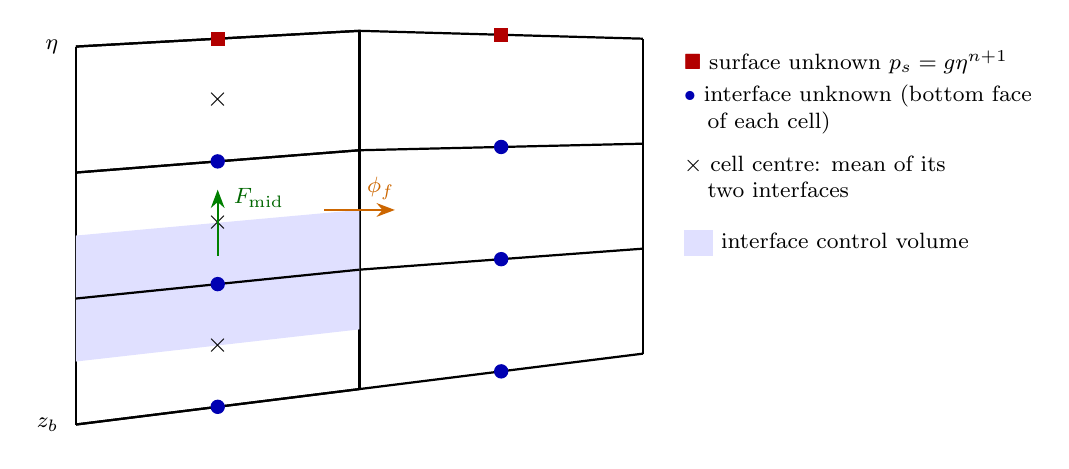
\begin{tikzpicture}[x=1cm,y=1cm,>=Stealth]
  % two columns, three layers, sloping bottom and surface
  \def\xa{0}\def\xb{3.6}\def\xc{7.2}
  \coordinate (b0) at (\xa,0.0);  \coordinate (b1) at (\xb,0.45); \coordinate (b2) at (\xc,0.9);
  \coordinate (s0) at (\xa,4.8);  \coordinate (s1) at (\xb,5.0);  \coordinate (s2) at (\xc,4.9);
  \foreach \k in {0,1,2,3} {
    \draw[thick] ($(b0)!\k/3!(s0)$) -- ($(b1)!\k/3!(s1)$) -- ($(b2)!\k/3!(s2)$);
  }
  \draw[thick] (b0) -- (s0); \draw[thick] (b1) -- (s1); \draw[thick] (b2) -- (s2);
  % interface CV of the middle interface of the left column (shaded)
  \fill[blue!12] ($(b0)!0.5/3!(s0)$) -- ($(b1)!0.5/3!(s1)$) -- ($(b1)!1.5/3!(s1)$) -- ($(b0)!1.5/3!(s0)$) -- cycle;
  \foreach \k in {0,1,2,3} {
    \draw[thick] ($(b0)!\k/3!(s0)$) -- ($(b1)!\k/3!(s1)$);
  }
  % interface unknowns (circles) at face centres of layer faces, surface unknowns (squares)
  \foreach \k in {0,1,2} {
    \fill[blue!70!black] ($($(b0)!\k/3!(s0)$)!0.5!($(b1)!\k/3!(s1)$)$) circle (2.6pt);
    \fill[blue!70!black] ($($(b1)!\k/3!(s1)$)!0.5!($(b2)!\k/3!(s2)$)$) circle (2.6pt);
  }
  \fill[red!70!black] ($($(s0)!0.5!(s1)$)+(-0.09,-0.09)$) rectangle +(0.18,0.18);
  \fill[red!70!black] ($($(s1)!0.5!(s2)$)+(-0.09,-0.09)$) rectangle +(0.18,0.18);
  % cell centres (crosses) of the left column
  \foreach \k in {0.5,1.5,2.5} {
    \node at ($($(b0)!\k/3!(s0)$)!0.5!($(b1)!\k/3!(s1)$)$) {$\times$};
  }
  % side flux, split half/half
  \draw[->,thick,orange!80!black] ($($(b1)!1.0/3!(s1)$)!0.5!($(b1)!2.0/3!(s1)$)+(-0.45,0)$) -- +(0.9,0)
     node[pos=0.8,above,font=\footnotesize,text=orange!80!black]{$\phi_{f}$};
  % mid-plane vertical flux
  \draw[->,thick,green!50!black] ($($(b0)!1.5/3!(s0)$)!0.5!($(b1)!1.5/3!(s1)$)+(0,-0.42)$) -- +(0,0.84);
  \node[font=\footnotesize,green!40!black,anchor=west] at ($($(b0)!1.5/3!(s0)$)!0.5!($(b1)!1.5/3!(s1)$)+(0.08,0.32)$) {$F_{\mathrm{mid}}$};
  % labels
  \node[font=\footnotesize,anchor=east] at ($(s0)+(-0.1,0)$) {$\eta$};
  \node[font=\footnotesize,anchor=east] at ($(b0)+(-0.1,0)$) {$z_b$};
  \node[font=\footnotesize,anchor=west,align=left] at (7.6,4.6)
     {\textcolor{red!70!black}{$\blacksquare$} surface unknown $p_s=g\eta^{n+1}$};
  \node[font=\footnotesize,anchor=west,align=left] at (7.6,4.0)
     {\textcolor{blue!70!black}{$\bullet$} interface unknown (bottom face\\ \quad of each cell)};
  \node[font=\footnotesize,anchor=west,align=left] at (7.6,3.15)
     {$\times$ cell centre: mean of its\\ \quad two interfaces};
  \node[font=\footnotesize,anchor=west,align=left] at (7.6,2.3)
     {\colorbox{blue!12}{\phantom{x}} interface control volume};
\end{tikzpicture}
\caption{Pressure on the layer interfaces: two columns of three layers. Each
interface carries one unknown; the shaded volume, half a cell below and half a
cell above an interface, is where continuity is imposed. A side flux $\phi_f$
is shared equally by the interfaces below and above it, and the flux
$F_{\mathrm{mid}}$ through the sloping mid-plane of a cell connects its two
interfaces.}
\label{fig:interface}
\end{figure}

\paragraph{Gradient.} Inside a cell, the vertical gradient is compact,
$(p_{\mathrm{top}}-p_{\mathrm{bot}})/\Delta z$. The value at the cell centre is
the mean of the two interfaces, and the horizontal gradient is the mean of the
two interface gradients, as in NHWAVE. In practice the momentum equation takes
the Gauss gradient with the interface values on the layer faces and the
interpolated centre values on the side faces.

\paragraph{Continuity.} Continuity is imposed on interface-centred control
volumes, half a cell below and half a cell above each interface, as in
NHWAVE's Poisson equation. With $\bm{H}/a_P$ the velocity predicted without the
pressure gradient and $r_A = 1/a_P$ the inverse of the momentum diagonal, the
flux through a side face $f$ between cells $P$ and $N$ is
\begin{equation}
  \phi_f = \phi^{*}_f - (r_A)_f\,|\bm{S}_f|\,\delta_f\left(\bar p_N - \bar p_P\right),
  \qquad \bar p = \tfrac12\left(p_{\mathrm{bot}} + p_{\mathrm{top}}\right),
  \label{eq:sideflux}
\end{equation}
so it couples the four interfaces of its two cells. Half of $\phi_f$ goes to
the control volume of the interface below and half to the one above. The flux
through the sloping mid-plane of cell $P$, of area vector
$\bm{S}_{\mathrm{mid}} = (S_x,S_y,A)$ with $A$ the horizontal area of the
column, connects the cell's two interfaces. It is split as OpenFOAM's
over-relaxed non-orthogonal Laplacian \citep{jasak1996}:
\begin{equation}
  F_{\mathrm{mid}} = \frac{\bm{H}}{a_P}\cdot\bm{S}_{\mathrm{mid}}
  - r_A\,\frac{A^2 + |\bm{S}_h|^2}{V}\,(p_{\mathrm{top}} - p_{\mathrm{bot}})
  - r_A\left[S_x\frac{\partial p}{\partial x} + S_y\frac{\partial p}{\partial y}
  - \frac{|\bm{S}_h|^2}{A}\frac{\partial p}{\partial z}\right]^{\mathrm{lagged}},
  \label{eq:midflux}
\end{equation}
where $|\bm{S}_h|^2 = S_x^2+S_y^2$ and $V$ is the cell volume. The implicit
coefficient carries the full $|\bm{S}_{\mathrm{mid}}|^2 = A^2 + |\bm{S}_h|^2$,
so the lagged bracket holds no vertical pressure difference, and the iteration
over the lagged terms converges however steep the layers are. With $A^2$ alone,
the pressure correctors diverged under the bore fronts of the breaking case
(Section~\ref{sec:breaking}).

\paragraph{Free surface.}
\label{sec:freesurface}
The control volume of the surface unknown is the upper half of the top cell.
Its outflow is the absolute flux through the surface face,
$\phi_s = A_h\,\partial\eta/\partial t$, discretised as
$A_h(\eta^{n+1}-\hat\eta)/a$ (Section~\ref{sec:time}). With
$\eta^{n+1}=p_s/g$ and the relaxation zones \eqref{eq:relax}, the equation of the
surface unknown of each column is
\begin{equation}
  \frac{A_h}{a}\left[(1 + a\sigma_r)\frac{p_s}{g} - \hat\eta - a\sigma_r\eta_t\right]
  = \tfrac12\sum_{\text{sides of the top cell}}\phi_f + F_{\mathrm{mid}} .
  \label{eq:surface}
\end{equation}
Each pressure solve therefore delivers $q$ and $\eta^{n+1}$ together. There is
no gravity-wave Courant limit, the matrix stays symmetric, and no pressure
reference is needed. After the solve, the side fluxes follow from
\eqref{eq:sideflux}, the fluxes through the layer faces are integrated upward
from the bed so that every cell conserves volume exactly, and
$\eta^{n+1}$ follows from the flux through the surface. In closed basins the
water volume is conserved to round-off.

\paragraph{Matrix and preconditioner.} The matrix of the interface unknowns is
symmetric positive definite, but it is not diagonally dominant where the
layers are thicker than the horizontal spacing, and incomplete Cholesky (DIC)
can then break down. \NHFOAM\ solves it with preconditioned conjugate gradients
and its own \code{sigmaColumn} preconditioner, which solves the tridiagonal
block of every column exactly (line relaxation in the vertical). It handles
thin layers and the strong vertical coupling of breaking columns, and falls
back to DIC (DILU for asymmetric matrices) on ordinary OpenFOAM matrices, so a
case can name it in either layout. Three kinds of terms would need more
couplings; they are lagged and updated in every non-orthogonal corrector:
\begin{enumerate}[nosep]
  \item the non-orthogonal correction of the side faces;
  \item the along-layer part of the mid-plane flux, the bracket in
        \eqref{eq:midflux};
  \item on processor boundaries, the couplings to the cell above the remote
        cell. The face is written in a compact form that bounds the exact one,
        and the difference is lagged.
\end{enumerate}

\subsection{Cell-centred pressure}
\label{sec:cellp}

With \code{pressureLocation cell}, $\prgh$ is OpenFOAM's usual cell-centred
field, and the kinematic and dynamic conditions combine into a Robin condition
on the surface patch, implemented through OpenFOAM's \code{mixed} patch field:
\begin{equation}
  p_s = f\,p_{\mathrm{ref}} + (1-f)\,p_c,\quad
  p_{\mathrm{ref}} = \frac{g\left(\hat\eta + a\sigma_r\eta_t + a\,\phi^{*}_s/A_h\right)}{1 + a\sigma_r},\quad
  f = \frac{1 + a\sigma_r}{1 + a\sigma_r + \beta_s},
  \label{eq:robin}
\end{equation}
with $\beta_s = g\,a\,(r_A)_f\,|\bm{S}_f|\,\delta_f/A_h$ and $p_c$ the value in the
top cell. This layout needs many more layers for the same dispersion
(Section~\ref{sec:dispersion}) and is kept for reference.

\subsection{Breaking columns}
\label{sec:numhfa}

In breaking columns the vertical coupling of the pressure is multiplied by a
large factor (\code{hydrostaticFactor}, default 1000). In the interface layout
this is the coefficient of $p_{\mathrm{top}}-p_{\mathrm{bot}}$ in
\eqref{eq:midflux}, up to the surface unknown; in the cell layout it is an
extra coupling across the layer faces plus a large mobility of the surface
face. $\prgh$ then becomes uniform in the vertical ($q=0$, since the surface
value is $g\eta$), and the fluxes through the layer faces follow from
continuity. The factor acts on the vertical pressure difference only: scaling
the face mobility itself would also scale the non-orthogonal correction on the
sloping layer faces, i.e.\ the horizontal pressure gradient under a steep
front, which drives spurious vertical fluxes.

The breaking flags, ages and eddy viscosities are set at the start of each
time step from $\partial\eta/\partial t = (\eta^n-\eta^{n-1})/\Delta t_0$.
The flags spread over the neighbouring columns in repeated sweeps until
nothing changes; on a processor they reach only the local columns. The
eddy viscosity of a face is the linear interpolate of the column values
(zero on walls, the free surface and the bottom, and on the closed faces of
dry columns), and the diffusion term is implicit in $\bm{u}$
(\code{fvm::laplacian}), so it needs no time-step limit.

\subsection{Time integration}
\label{sec:time}

Time integration follows the \code{ddt(U)} scheme: Euler, or the second-order
backward differentiation formula (BDF2) with variable time-step coefficients
for both $\bm{u}$ and $\eta$. With $r = \Delta t/\Delta t_0$, where $\Delta t_0$ is
the previous step,
\begin{equation}
  \begin{aligned}
  \left.\frac{\partial\eta}{\partial t}\right|^{n+1} &\approx \frac{\eta^{n+1}-\hat\eta}{a},\qquad
  a = \frac{\Delta t}{c},\qquad
  \hat\eta = \frac{c_0\,\eta^{n} - c_{00}\,\eta^{n-1}}{c},\\
  c &= 1 + \frac{r}{1+r},\qquad
  c_{00} = \frac{r^2}{1+r},\qquad
  c_0 = c + c_{00}.
  \end{aligned}
  \label{eq:bdf2}
\end{equation}
The first step after the start (or a restart) is Euler. OpenFOAM's Rhie--Chow
type time-derivative flux correction (\code{ddtCorr}) is used with its
coefficient set to one (\code{backward 1} in \code{ddtSchemes}); with the
default limiter, standing waves lost 3.9\% of their amplitude over 4.5
periods instead of 0.09\%.

\paragraph{Algorithm per time step.}
\begin{enumerate}[nosep]
  \item Shift the time levels of $\eta$ and of the face velocity $\bm{u}_f$; set the
        targets of the relaxation zones and the breaking flags.
  \item Move the mesh to the extrapolated surface
        $\eta^{*} = \eta^n + r\,(\eta^n - \eta^{n-1})$.
  \item Rebuild the flux on the moved faces from the face velocity and make
        it relative to the mesh motion. In the first outer corrector the face
        velocity is extrapolated (\code{fluxExtrapolation}, default on with
        BDF2):
        \begin{equation}
          \phi^{*} = \bm{S}_f\cdot\left[(1+r)\,\bm{u}_f^{n} - r\,\bm{u}_f^{n-1}\right] - \phi_{\mathrm{mesh}} .
          \label{eq:fluxext}
        \end{equation}
  \item Momentum predictor, with the pressure gradient of the last corrector.
  \item Pressure correctors (\code{nCorrectors}, 2--3). Each one assembles and
        solves the interface matrix with the surface rows \eqref{eq:surface}
        (or, in the cell layout, sets the Robin coefficients \eqref{eq:robin}
        and solves for $\prgh$), with \code{nNonOrthogonalCorrectors} updates
        of the lagged terms, then updates the flux, $\eta^{n+1}$, $\bm{u}$ and
        $\bm{u}_f$.
  \item Optional further outer correctors repeat steps 3--5 with the latest
        flux (and, with \code{moveMeshOuterCorrectors}, the latest $\eta$).
\end{enumerate}

\paragraph{Order of accuracy in time.} With one outer corrector, the momentum
equation of step $n+1$ is linearised with a convecting flux of level $n$. That
lag is an error of order $\Delta t$ in every step, so the scheme is only first
order in time for nonlinear waves, although BDF2 is second order. In the
solitary wave of Section~\ref{sec:ma-solitary}, halving the time step halved
the error. The extrapolation \eqref{eq:fluxext} removes the lag at no cost.
Before it was introduced, a second outer corrector gave the same accuracy at
1.6 times the cost (Section~\ref{sec:ma-solitary}).

\subsection{Convection}
\label{sec:convection}

The convection term uses OpenFOAM's schemes. Three are used in this report:
\begin{itemize}[nosep]
  \item \code{Gauss limitedLinearV 1}, a TVD scheme. It is needed in breaking
        cases, where bores form, and it was the default until this report;
  \item \code{Gauss filteredLinear2V 0.2 0}, central differencing with a filter
        that only acts on grid-scale oscillations. It damps waves as little as
        central differencing but stayed stable in long nonlinear runs
        (Section~\ref{sec:ma}); it is the recommended scheme for non-breaking
        waves;
  \item \code{Gauss linear}, pure central differencing. It damps least, but
        grid-scale noise grows in long nonlinear runs and behind bores.
\end{itemize}
Upwind-biased schemes (\code{linearUpwind}, \code{LUST}) damp waves of moderate
steepness noticeably (Section~\ref{sec:convtests}).

\section{Verification and comparison with NHWAVE and REEF3D::NHFLOW}
\label{sec:verification}

This section collects the first round of tests. Where possible, the
benchmarks were also run with two established non-hydrostatic $\sigma$-layer
models on the same set-up: the same domain, bottom, gauges, horizontal spacing
and number of layers. Each model keeps its own numerics and its usual wave
input (Table~\ref{tab:models}). Unless stated otherwise, \NHFOAM\ uses the
interface pressure, \code{limitedLinearV}, BDF2 and one outer corrector without
flux extrapolation, i.e.\ the settings before the fixes of
Section~\ref{sec:ma2012}.

\begin{table}[ht]
\centering
\caption{The three models compared in Sections~\ref{sec:verification} and
\ref{sec:ma2012}.}
\label{tab:models}
\small
\begin{tabular}{p{3.0cm}p{3.6cm}p{3.6cm}p{3.6cm}}
\toprule
 & \NHFOAM & NHWAVE & REEF3D::NHFLOW \\
\midrule
version & this repository & \code{JimKirby/NHWAVE} master (1483007), MPI and HYPRE 3.2 & 26.08 (conda-forge build) \\
vertical pressure & layer interfaces (default) or cell centres & layer interfaces & as distributed \\
advection, time & see text; BDF2 & HLPA (TVD), second-order Runge--Kutta & WENO, HLL fluxes \\
time step (bar) & fixed, 5 ms & adaptive, CFL 0.5 ($\approx$4.6 ms) & adaptive, CFL 1 ($\approx$9.7 ms) \\
wave input (bar) & 8 m relaxation zone, linear & linear, at the left boundary & 8 m relaxation zone, linear \\
absorption (bar) & 8 m sponge & 8 m sponge & 8 m relaxation zone \\
\bottomrule
\end{tabular}
\end{table}

\subsection{Basic checks}
\label{sec:basic}

Table~\ref{tab:basic} lists the basic checks; Figs.~\ref{fig:basin3d} and
\ref{fig:solitary01} show two of them.

\begin{table}[ht]
\centering
\caption{Basic checks (interface pressure unless noted).}
\label{tab:basic}
\small
\begin{tabular}{p{6.3cm}p{8.7cm}}
\toprule
test & result \\
\midrule
still water over the bar bathymetry (1:20 and 1:10 slopes), 10 s & $\eta\equiv 0$ (exact); $\max|\bm{u}| < 10^{-12}$ m/s, exactly 0 at the end \\
volume conservation, closed basins & round-off: $10^{-14}$ m$^3$ or less (2DV and 3D) \\
standing wave, $kh=1$, 10 layers, $T/\Delta t = 200$ & period $+0.04\%$, amplitude $-0.04\%$ over $4.5\,T$ (cell layout $+0.13\%$, $-0.03\%$) \\
solitary wave, $H/h = 0.1$, 10 layers & speed 3.283 m/s between $x=10$ and 30 m, against $\sqrt{g(h+H)} = 3.285$ m/s; height $-0.2\%$ from $x=10$ to 40 m \\
circular basin, 3D unstructured prisms, 8 layers & period $+0.07\%$ against the analytical Bessel mode (cell layout $+0.20\%$) \\
serial vs 2 processors (solitary wave crossing the processor boundary) & $\max|\Delta\eta| = 7\times10^{-8}$ m for $H = 0.1$ m \\
bottom uplift, $\zeta_0/h = 0.01$, 5 layers & peaks within 1.5\% of linear potential theory up to $x/b = 20$; volume conserved to $10^{-16}$ m$^3$ \\
\bottomrule
\end{tabular}
\end{table}

\begin{figure}[ht]
\centering
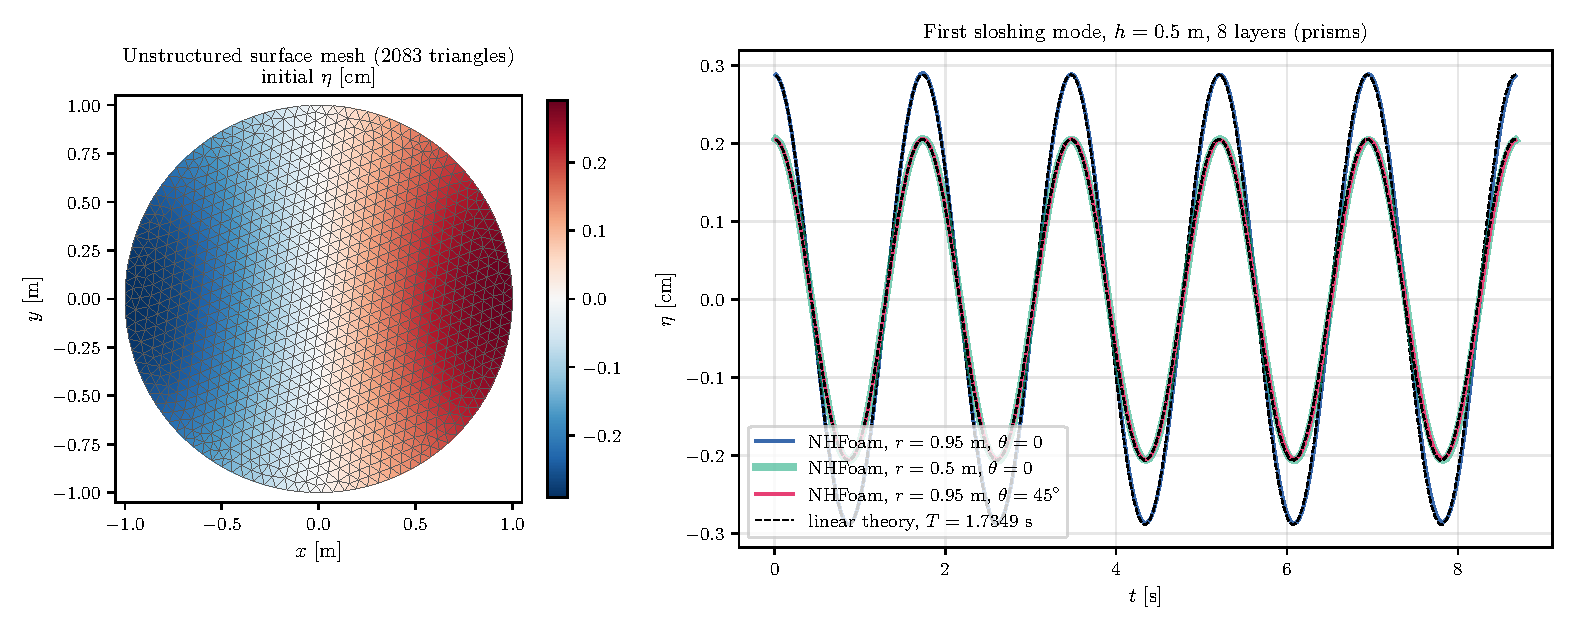
\includegraphics[width=\textwidth]{circular_basin_3d.pdf}
\caption{First sloshing mode of a circular basin ($R=1$ m, $h=0.5$ m) on an
unstructured mesh of triangular prisms, 8 layers: surface mesh with the
initial elevation, and gauges against linear theory.}
\label{fig:basin3d}
\end{figure}

\begin{figure}[ht]
\centering
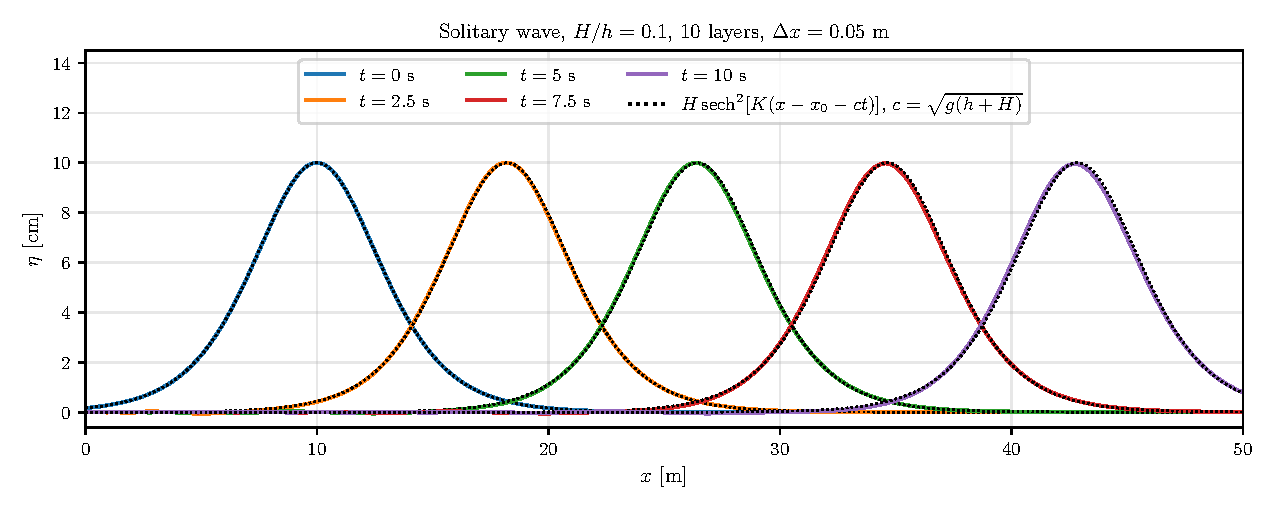
\includegraphics[width=\textwidth]{solitary_wave.pdf}
\caption{Solitary wave of $H/h=0.1$, 10 layers, $\Delta x = 0.05$ m: profiles
against the initial $\mathrm{sech}^2$ shape moved at $c=\sqrt{g(h+H)}$.}
\label{fig:solitary01}
\end{figure}

\FloatBarrier
\subsection{Dispersion and the number of layers}
\label{sec:dispersion}

Standing waves in closed basins, with 64 cells per wavelength,
$T/\Delta t = 200$ and uniform layers, give the period error of
Table~\ref{tab:dispersion} and Fig.~\ref{fig:dispersion}, measured over 4.5
periods. With the pressure on the interfaces, two layers keep the period error
within 0.6\% up to $kh=7$ and three layers within 0.21\%. With five or more
layers, what is left ($-0.04$ to $+0.07\%$) comes from $\Delta x$ and $\Delta t$.
The cell-centred layout needs about 3 layers for $kh\le1$, 5--6 for $kh\le2$,
10 for $kh\le4$ and 20 for $kh\le7$ to stay within 1\%.

\begin{table}[ht]
\centering
\caption{Period error of standing waves [\%] for $kh = 1$ / 3 / 7.}
\label{tab:dispersion}
\small
\begin{tabular}{rll}
\toprule
layers & interface layout (default) & cell layout \\
\midrule
1  & $-2.4$ / $+3.9$ / $+38$       & $+6.9$ / $+35$ / $+91$ \\
2  & $-0.52$ / $-0.16$ / $+0.61$   & $+1.9$ / $+12$ / $+42$ \\
3  & $-0.20$ / $-0.06$ / $+0.05$   & $+0.88$ / $+5.9$ / $+24$ \\
5  & $-0.03$ / $+0.01$ / $+0.05$   & $+0.36$ / $+2.2$ / $+10.5$ \\
10 & $+0.04$ / $+0.04$ / $+0.05$   & $+0.13$ / $+0.61$ / $+3.0$ \\
20 & $+0.06$ / $+0.05$ / $+0.04$   & $+0.08$ / $+0.19$ / $+0.79$ \\
\bottomrule
\end{tabular}
\end{table}

\begin{figure}[ht]
\centering
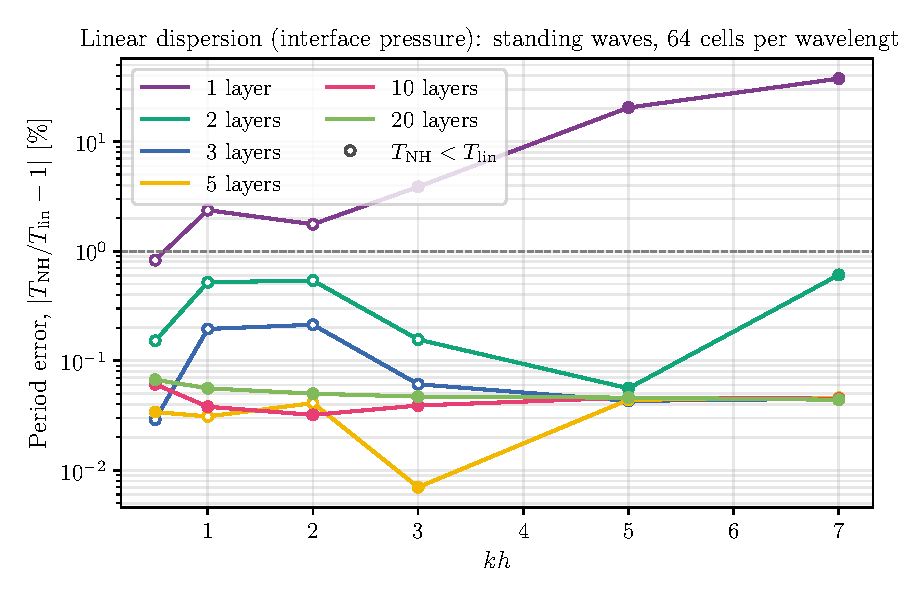
\includegraphics[width=0.85\textwidth]{dispersion_vs_layers.pdf}
\caption{Period error of standing waves against $kh$ for 1--20 uniform layers
(interface pressure). Open symbols: periods shorter than linear theory.}
\label{fig:dispersion}
\end{figure}

Refining the layers towards the surface no longer helps
(Fig.~\ref{fig:grading}). With three layers, a top layer a quarter of the
bottom one moves the error at $kh = 1$--2 from $-0.2\%$ to $-0.45\%$, and at
$kh=5$ it stays at $+0.05\%$. In the cell layout the same grading cut the error
at $kh=5$ from 5.8\% to 2.1\% with five layers.

\begin{figure}[ht]
\centering
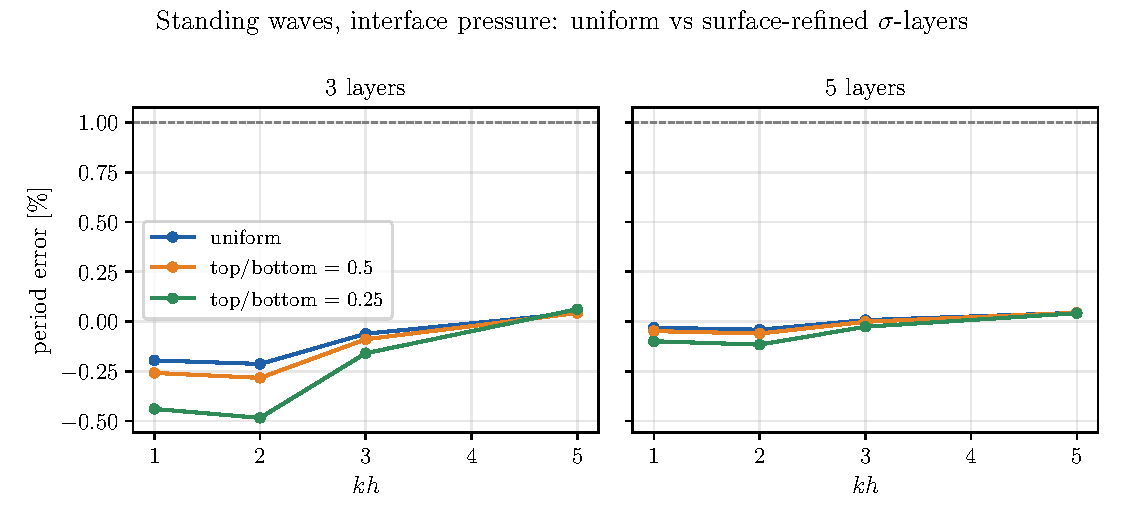
\includegraphics[width=\textwidth]{layer_grading.pdf}
\caption{Period error with uniform and surface-refined layers (interface
pressure).}
\label{fig:grading}
\end{figure}

Against NHWAVE, on the same basins and with the same analysis
(Fig.~\ref{fig:dispmodels}), NHWAVE keeps the period error within 0.8\% with
two layers and 0.45\% with three; \NHFOAM\ within 0.61\% and 0.21\%. With
10--20 layers both converge, NHWAVE to $-0.17\%$ and \NHFOAM\ to $+0.05\%$.
NHWAVE damps more: after 4.5 periods it has lost 0.6--12\% of the amplitude
with three layers and 0.6--3.5\% with ten, \NHFOAM\ 0.04--1.3\% and
0.04--0.7\%.

\begin{figure}[ht]
\centering
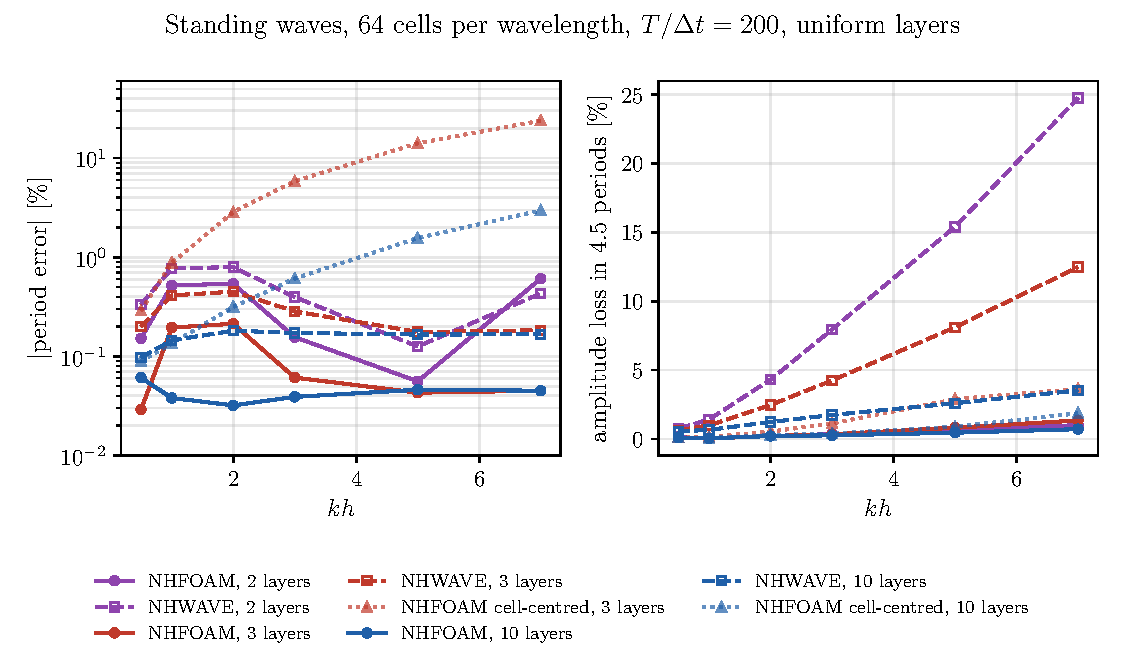
\includegraphics[width=\textwidth]{dispersion_models.pdf}
\caption{Standing waves: period error and amplitude loss of \NHFOAM\ (interface
and cell-centred pressure) and NHWAVE for 2, 3 and 10 uniform layers.}
\label{fig:dispmodels}
\end{figure}

\FloatBarrier
\subsection{Convection and the decay of progressive waves}
\label{sec:convtests}

Waves of $H=4.1$ cm and $T=1.01$ s in 0.4 m of water ($kh = 1.69$, 10 layers,
$\Delta x = 2$ cm) lose 6.1\% of their height over 12 m (8 wavelengths) with
\code{linearUpwind}, 4.7\% with \code{LUST}, 4.4\% with \code{limitedLinearV}
and 3.9\% with central differencing (Fig.~\ref{fig:flume}). With the
cell-centred pressure the same runs lost 12\%, 6.2\%, 3.3\% and 1.7\%. Waves of
$H = 0.4$ cm lose 0.7\% over 10 m with \code{linearUpwind}, so the damping grows
with steepness. The waves leave the wave-making zone about 4\% higher than the
linear target, a nonlinear effect of generating them with linear theory. The
phase speed of the small waves is 0.24\% below linear theory (10 layers,
$T/\Delta t = 100$), of which about 0.13\% is the BDF2 time step. These runs
predate the flux extrapolation of Section~\ref{sec:time}.

\begin{figure}[ht]
\centering
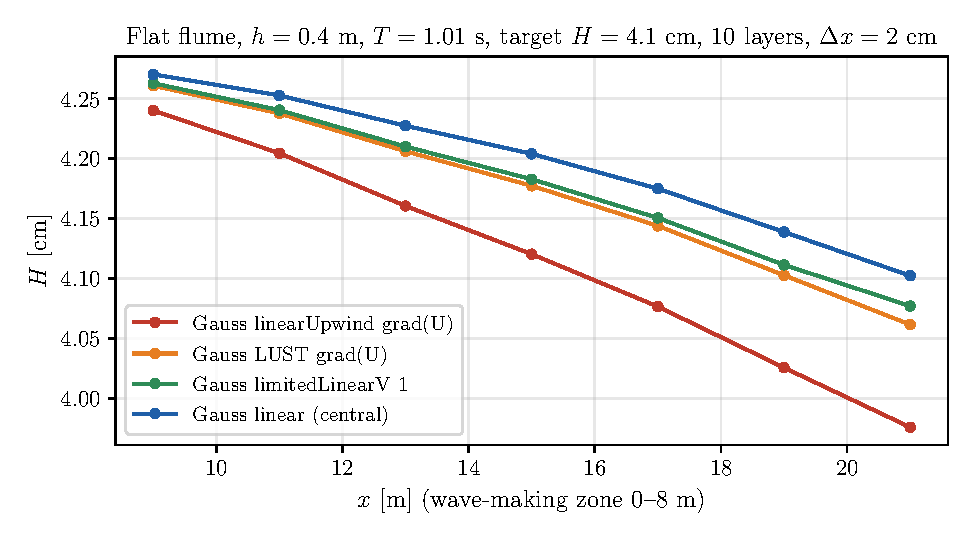
\includegraphics[width=0.85\textwidth]{flume_convection.pdf}
\caption{Wave height along a flat flume for four convection schemes (interface
pressure).}
\label{fig:flume}
\end{figure}

\FloatBarrier
\subsection{Submerged bar}
\label{sec:bar10}

Periodic waves over the submerged bar of \citet{beji1993}, in the version of
\citet{luth1994} with its cases A ($H = 2$ cm, $T = 2.02$ s) and C
($H=4.1$ cm, $T=1.01$ s), test shoaling and the release of free higher
harmonics behind the bar. All three models use $\Delta x = 2$ cm and 10 uniform
layers; \NHFOAM\ uses $\Delta t = 5$ ms. One time shift, fitted at $x=22$ m, is
applied to all gauges of a run, and $\Delta H$ is the error of the wave height
(max $-$ min over the lab record). All runs are compared over the last 4 s
before $t=50$ s (Figs.~\ref{fig:barA} and \ref{fig:barC},
Table~\ref{tab:bar10}).

\begin{table}[ht]
\centering
\caption{Submerged bar, 10 layers: rms error over the 10 gauges and mean
$|\Delta H|/H$, window ending at $t = 50$ s.}
\label{tab:bar10}
\small
\begin{tabular}{lcccc}
\toprule
 & \NHFOAM & \NHFOAM, cell layout & NHWAVE & REEF3D::NHFLOW \\
\midrule
case A, rms        & 0.17 cm & 0.21 cm & 0.29 cm & 0.24 cm \\
case A, $|\Delta H|/H$ & 5.1\% & 6.6\% & 4.7\% & 6.3\% \\
case C, rms        & 0.65 cm & 0.59 cm & 1.02 cm & 0.92 cm \\
case C, $|\Delta H|/H$ & 4.9\% & 4.7\% & 6.1\% & 5.1\% \\
\bottomrule
\end{tabular}
\end{table}

\begin{figure}[p]
\centering
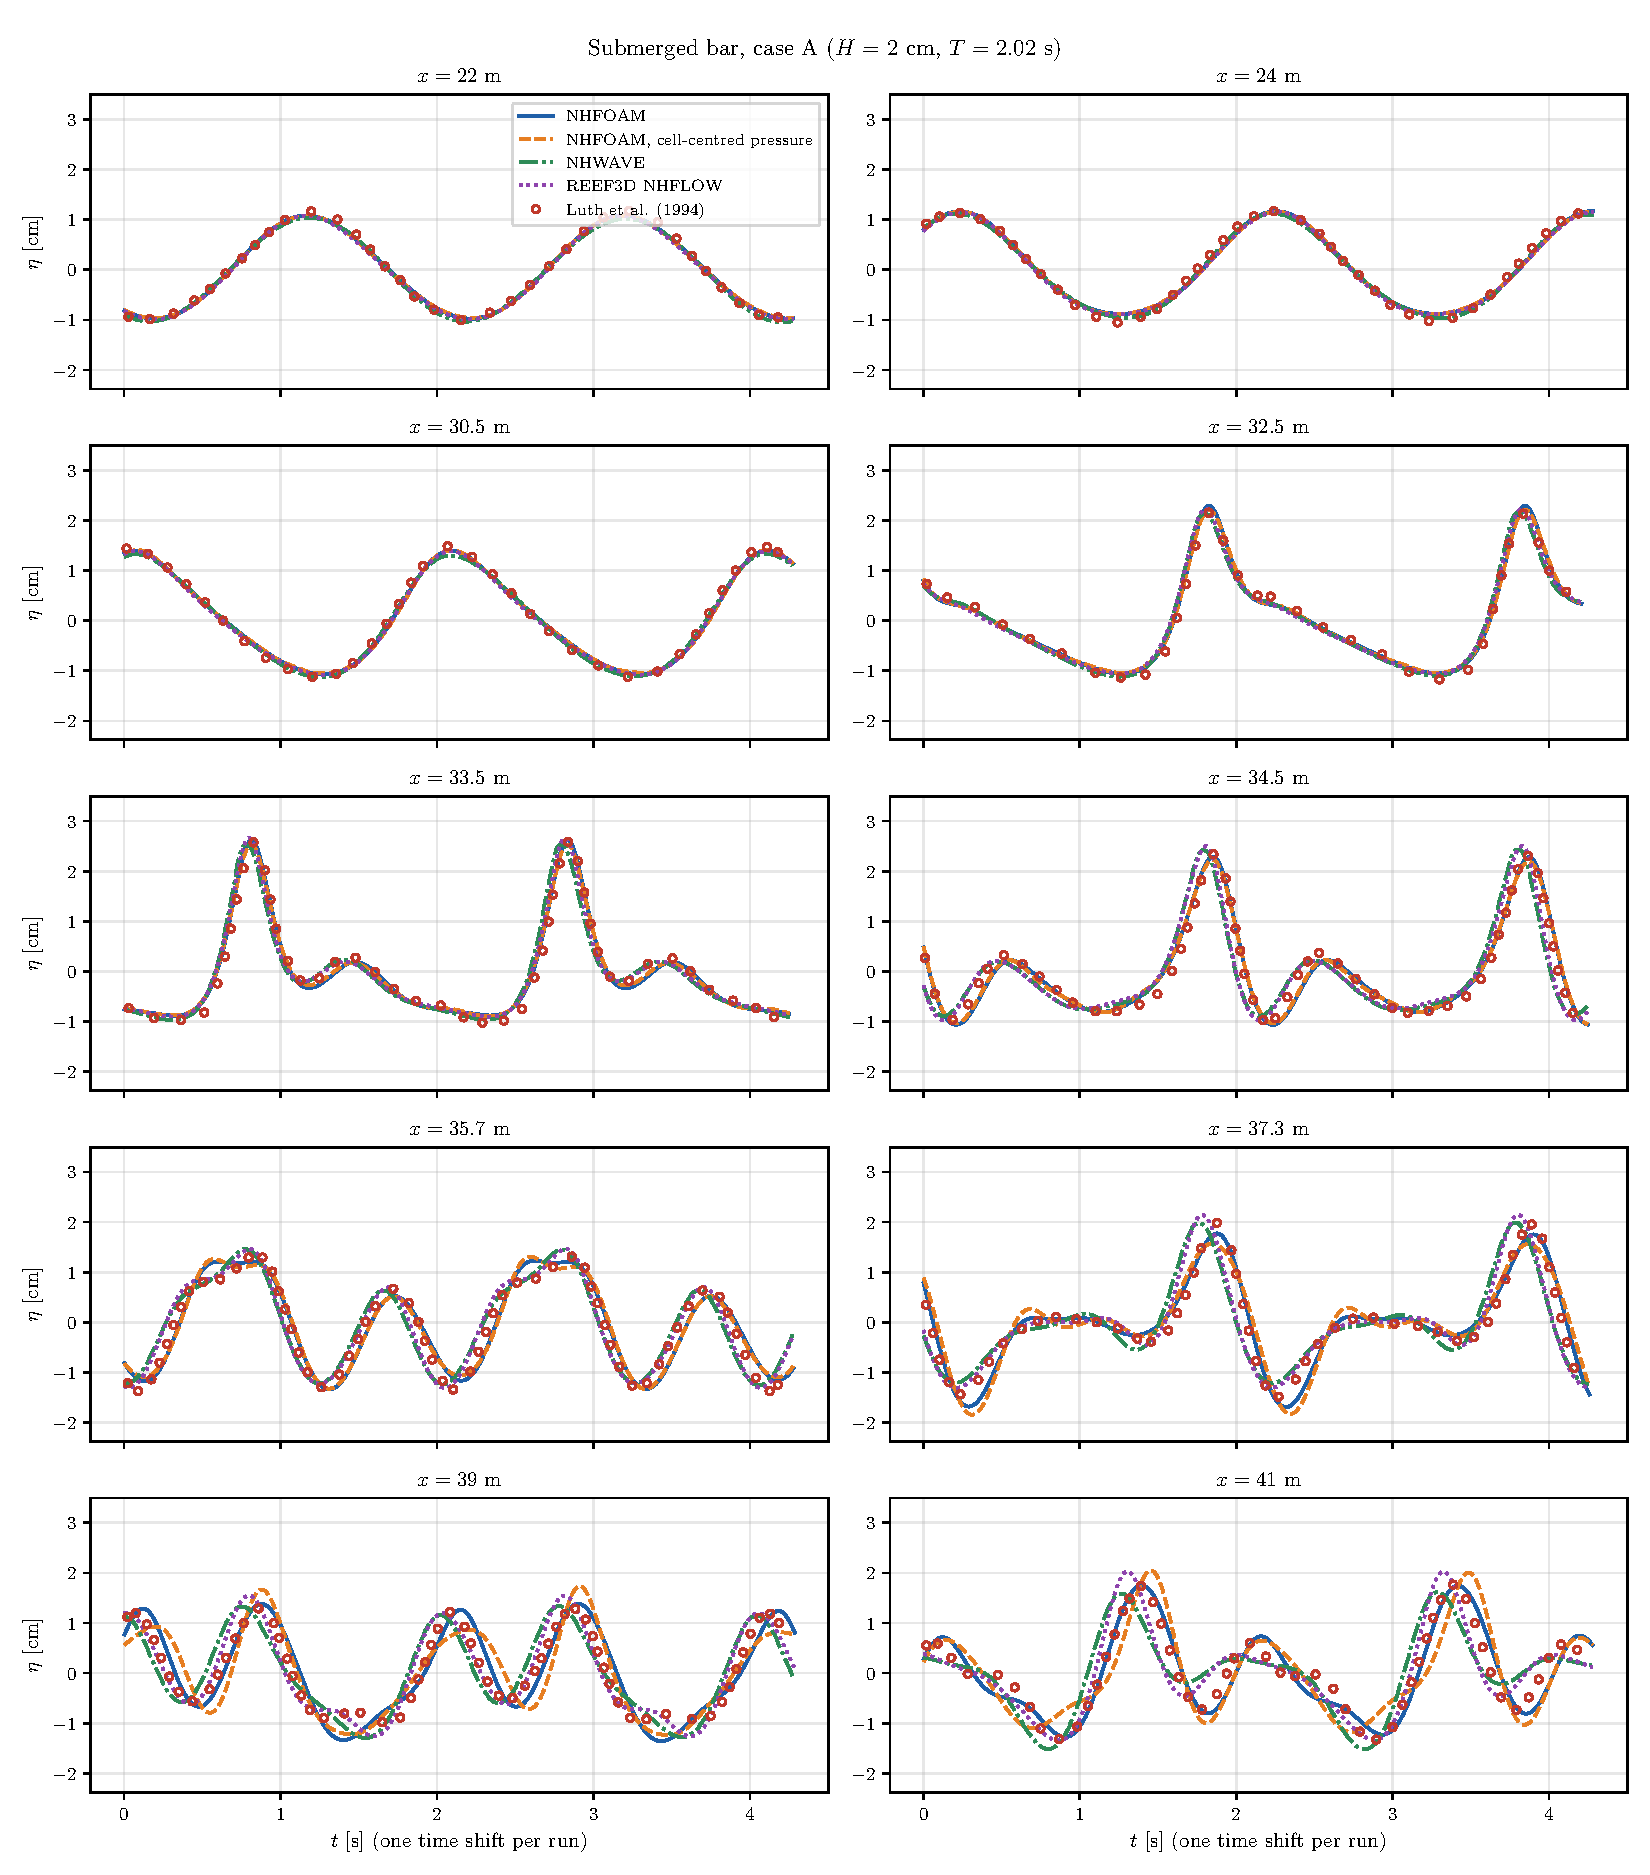
\includegraphics[width=0.9\textwidth]{bar_models_A.pdf}
\caption{Submerged bar, case A, 10 layers: \NHFOAM\ (interface and cell-centred
pressure), NHWAVE and REEF3D::NHFLOW against \citet{luth1994}.}
\label{fig:barA}
\end{figure}

\begin{figure}[p]
\centering
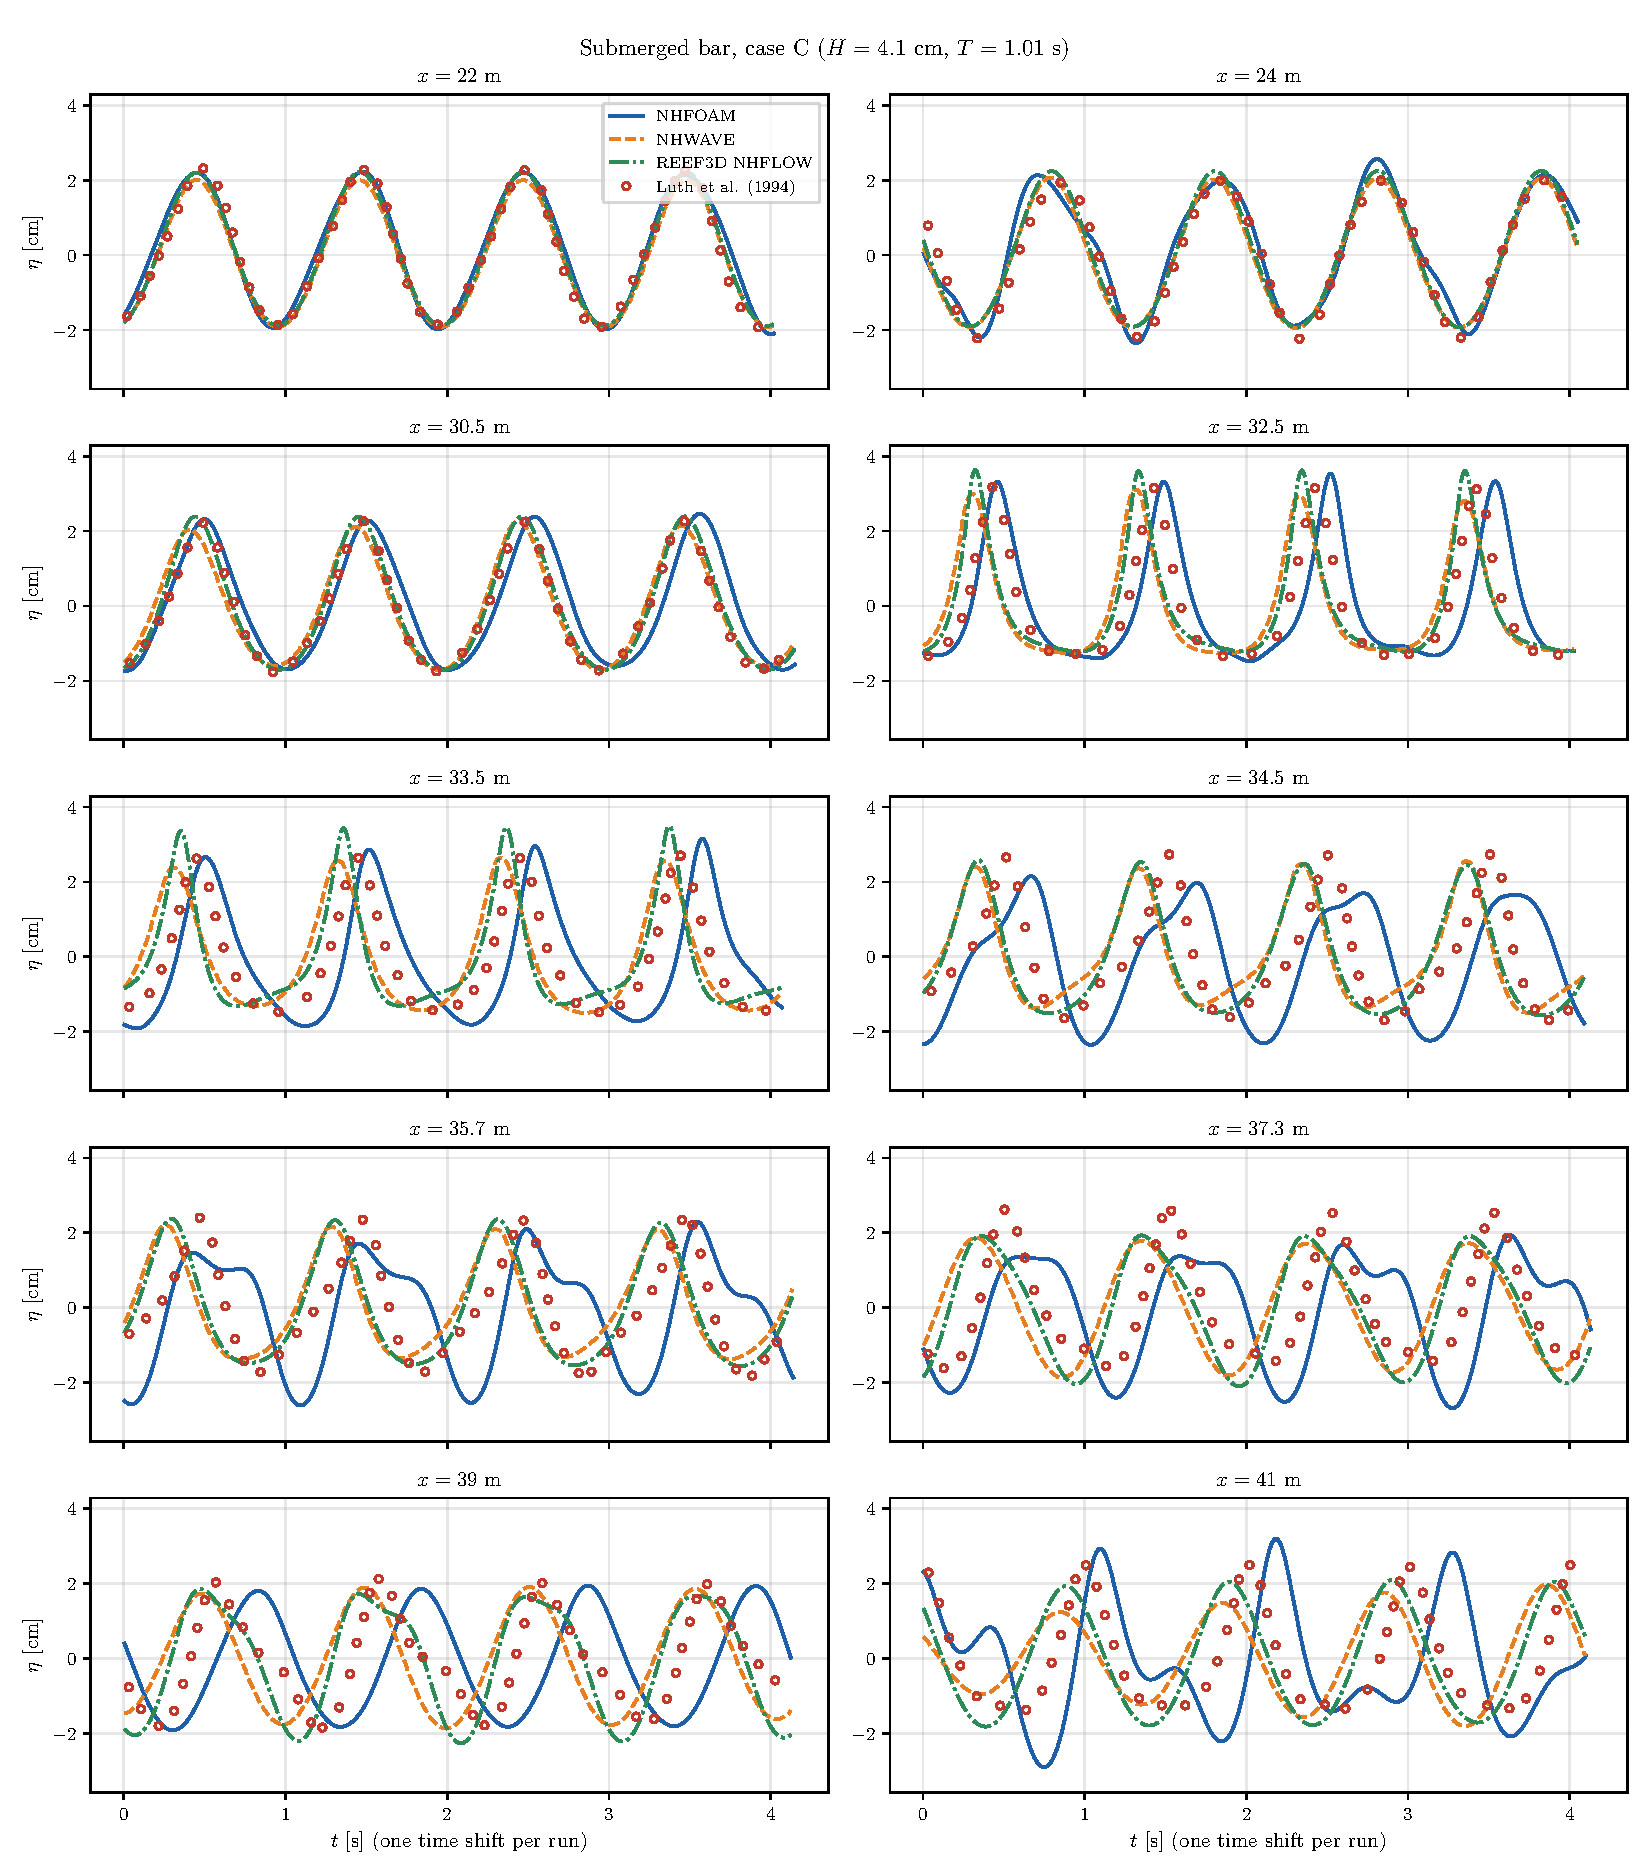
\includegraphics[width=0.92\textwidth]{bar_models_C.pdf}
\caption{As Fig.~\ref{fig:barA}, case C.}
\label{fig:barC}
\end{figure}

In front of the bar ($x\le 30.5$ m) all models are within 0.06--0.42 cm rms of
the measurements. On and behind the bar, \NHFOAM\ has the smallest errors at
every gauge in case C (0.46--0.90 cm, against 1.0--1.5 cm for the other two)
and at 6 of the 7 gauges in case A. In case C the difference is mostly phase:
NHWAVE and REEF3D::NHFLOW are 0.1--0.18 s early over the bar crest, and
\NHFOAM\ up to 0.1 s late.

\paragraph{Long waves of the flume.} The phase over the bar changes with the
time at which it is measured, in all three models. Between $t=45$ and 65 s, the
first harmonic at $x = 35.7$ m moves relative to $x=22$ m by 0.21 s in \NHFOAM,
0.08 s in NHWAVE and $-0.07$ s in REEF3D::NHFLOW. These changes come with mean
water levels that vary by a few millimetres along the flume ($\pm2$ mm in
\NHFOAM, $\pm1$ mm in the other two): long waves of the closed flume, released
when the wave train starts and when it crosses the bar, which the zones absorb
only partly. Over the 0.1 m deep crest the current of such a wave shifts the
waves by tenths of a second, so the rms error depends on the window
(Table~\ref{tab:barwindow}), and so does the ranking. The drift was later
traced to the missing return current of the wave-making zone; with it, the
runs are steady (Section~\ref{sec:bar-bc}).

\begin{table}[ht]
\centering
\caption{Case C, 10 layers: rms error over the 10 gauges for windows ending at
different times.}
\label{tab:barwindow}
\small
\begin{tabular}{lcccc}
\toprule
window ending at & \NHFOAM & \NHFOAM, cell layout & NHWAVE & REEF3D::NHFLOW \\
\midrule
45 s & 0.49 cm & 0.47 cm & 1.08 cm & 0.93 cm \\
50 s & 0.65 cm & 0.59 cm & 1.02 cm & 0.92 cm \\
55 s & 0.94 cm & 0.77 cm & 0.97 cm & 0.92 cm \\
60 s & 1.18 cm & 1.04 cm & 0.89 cm & 0.98 cm \\
65 s & 1.39 cm & 1.19 cm & 0.77 cm & 1.10 cm \\
\bottomrule
\end{tabular}
\end{table}

Two numerical settings matter as much as the model (cell layout, 50 s
windows). With $\Delta t = 10$ ms instead of 5 ms the rms error was 65\% higher
in case A and 150\% higher in case C: the free third harmonic behind the bar
($T/3 = 0.34$ s in case C) then gets only 34 steps per period. And central
differencing failed after 62 s (case A) and 53 s (case C), while
\code{limitedLinearV} runs to the end.

\FloatBarrier
\subsection{Seabed motion}
\label{sec:seabed}

\paragraph{Bottom uplift.} A block of half-width $b=0.305$ m rises by
$\zeta_0 = 0.5$ mm in $h=5$ cm of water with the exponential history
($t_c = 0.1$ s), as in \citet{hammack1973}. With 5 layers and $\Delta x = 5$ mm the
peaks at $x/b = 0$--20 are within 1.5\% of linear potential theory, and the
dispersive tail follows it (Fig.~\ref{fig:uplift}). The two pressure layouts
differ by less than 2\% of $\zeta_0$ at any gauge.

\begin{figure}[ht]
\centering
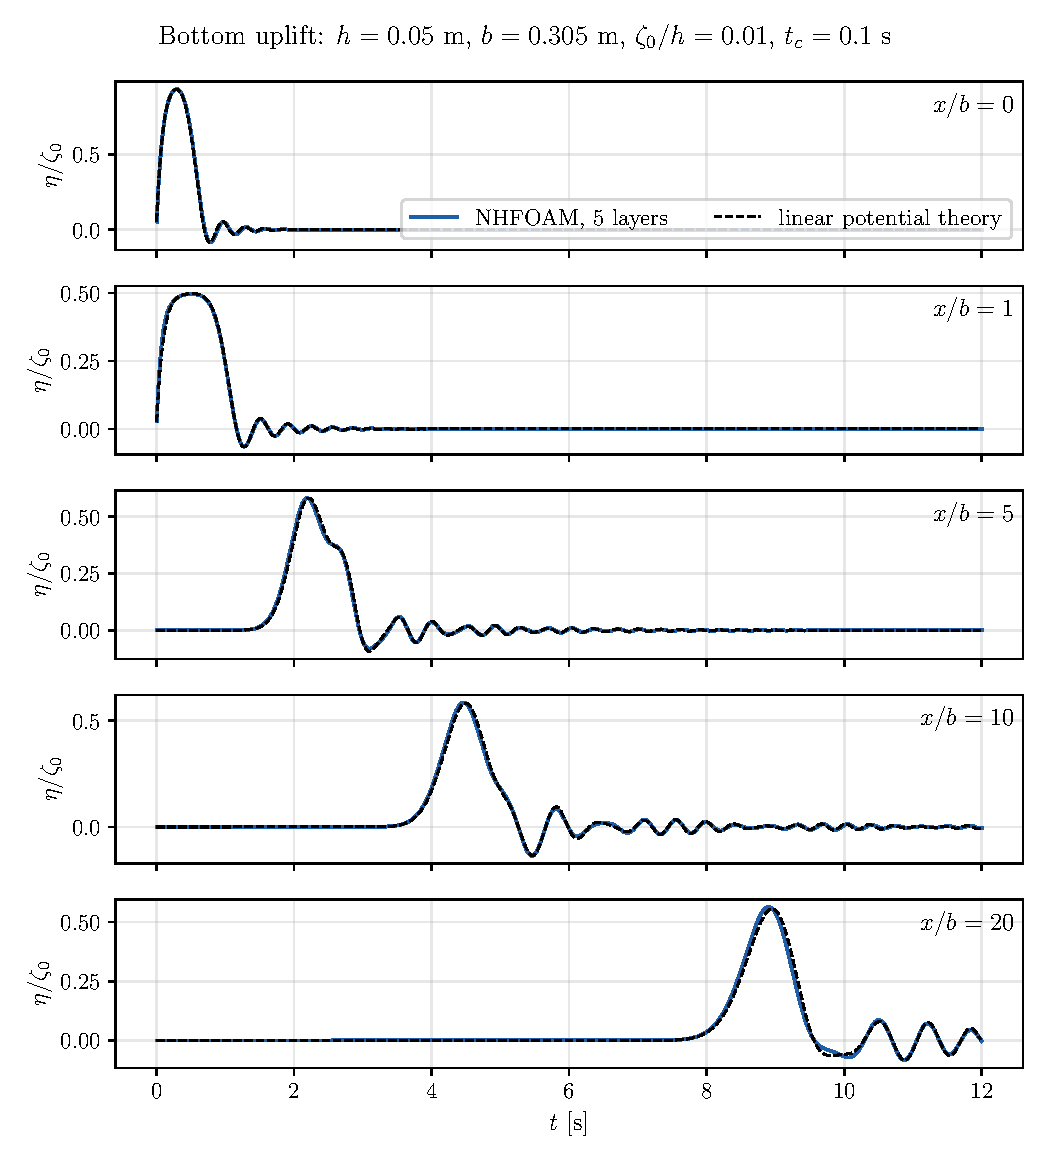
\includegraphics[width=0.8\textwidth]{bottom_uplift.pdf}
\caption{Bottom uplift: gauges against linear potential theory.}
\label{fig:uplift}
\end{figure}

\paragraph{3D rigid landslide.} NTHMP benchmark 2 \citep{enet2007}, $d = 61$ mm:
half tank with a symmetry wall on the axis. \NHFOAM: $\Delta x=\Delta y=2.5$ cm,
5 uniform layers (141\,000 cells), the domain starting 0.2 m from the shoreline
(no wetting and drying). In deep water the layers are up to 12 times thicker
than $\Delta x$, so the interface matrix needs about 180 PCG iterations per solve,
and the run takes 51 min on one core for 4 s. NHWAVE uses its own benchmark
set-up (\code{examples/landslide\_benchmarks/BM2\_enet\_grilli}: $\Delta x = 2$ cm,
3 layers, full beach), with the gauges moved to the published positions. No
time shift is applied (Fig.~\ref{fig:landslide}, Table~\ref{tab:landslide}).

\begin{table}[ht]
\centering
\caption{Landslide, $d=61$ mm: first trough and first crest [mm].}
\label{tab:landslide}
\small
\setlength{\tabcolsep}{4pt}
\begin{tabular}{lcccccccc}
\toprule
 & \multicolumn{4}{c}{first trough} & \multicolumn{4}{c}{first crest} \\
\cmidrule(lr){2-5}\cmidrule(lr){6-9}
gauge $(x,y)$ [m] & lab & \NHFOAM & cell & NHWAVE & lab & \NHFOAM & cell & NHWAVE \\
\midrule
g2 (1.469, 0.35) & $-13.7$ & $-15.3$ & $-14.9$ & $-14.9$ & 15.0 & 16.7 & 15.2 & 16.3 \\
g3 (1.929, 0)    & $-17.0$ & $-17.7$ & $-18.0$ & $-17.1$ & 22.2 & 23.9 & 22.5 & 20.5 \\
g4 (1.919, 0.5)  & $-9.4$  & $-10.2$ & $-9.5$  & $-9.6$  & 11.0 & 13.0 & 11.6 & 12.3 \\
\bottomrule
\end{tabular}
\end{table}

\begin{figure}[ht]
\centering
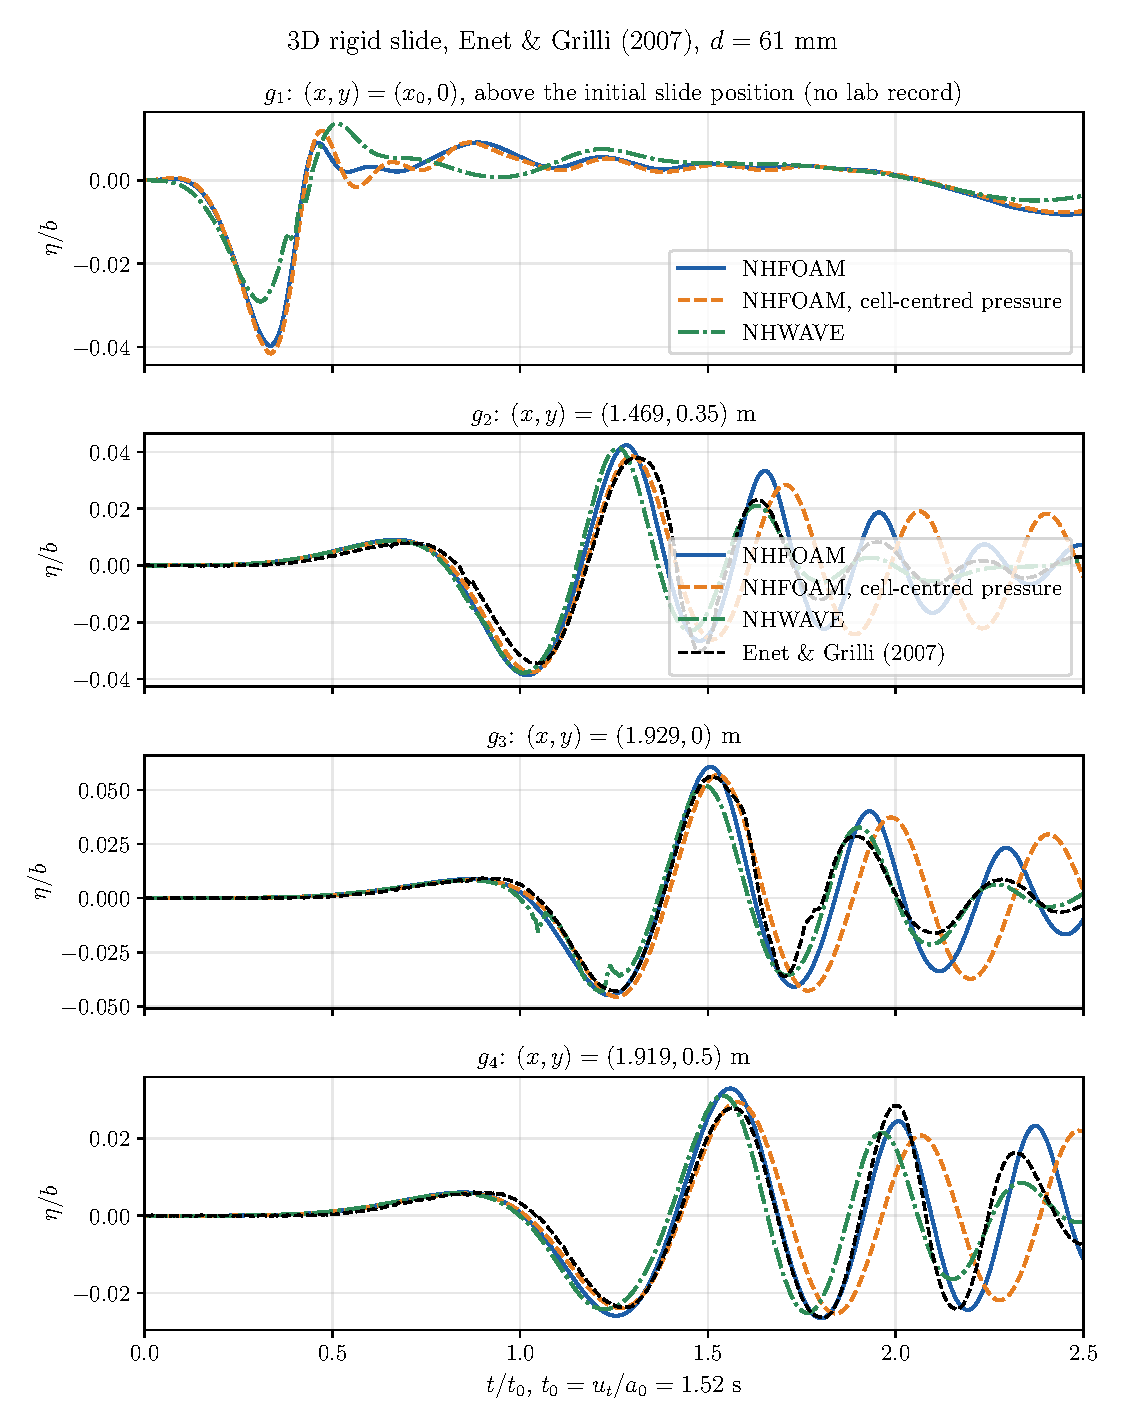
\includegraphics[width=0.85\textwidth]{landslide_models.pdf}
\caption{3D rigid landslide \citep{enet2007}, $d=61$ mm: \NHFOAM\ (interface and
cell-centred pressure) and NHWAVE against the measurements.}
\label{fig:landslide}
\end{figure}

All runs get the leading trough within 12\%. The leading crest is 8--18\% high
with the interface pressure, 1--5\% with the cell-centred pressure, and
between $-7\%$ and $+12\%$ for NHWAVE. \NHFOAM\ has the leading waves on time,
NHWAVE about $0.05\,t_0$ early. The trailing waves ($kh = 3$--5) now follow the
measured phase, as NHWAVE's do; with the cell-centred pressure they fell
further behind with every wave. Their amplitude is still too large: the third
and fourth crests are up to 2--3 times the measured ones, while NHWAVE follows
the measured decay. The wall that replaces \NHFOAM's beach is not the cause
(Section~\ref{sec:ma-landslide}).

\FloatBarrier
\subsection{Breaking}
\label{sec:breaking}

Spilling breakers of \citet{hansen1979}, test 061071: $T = 1.67$ s, $H = 6.9$ cm
at the toe of a 1:34.26 slope from $h=0.36$ m. 10 layers, $\Delta x = 2$ cm,
$\Delta t = 10$ ms, HFA with $\alpha = 0.6$ and $\beta=0.3$, \code{limitedLinearV}.
The slope is cut at $x = 11$ m ($h = 3.9$ cm) and continues as a 3 m shelf with
a velocity-only sponge. The run covers 40 periods, and the statistics use the
last 10 (Fig.~\ref{fig:hs}, Table~\ref{tab:hs}).

\begin{table}[ht]
\centering
\caption{Spilling breakers: wave height (mean of max $-$ min per period).}
\label{tab:hs}
\small
\begin{tabular}{llll}
\toprule
 & lab & \NHFOAM\ (interface) & \NHFOAM\ (cell) \\
\midrule
near the toe, $x<1$ m & 6.9--7.0 cm & $-1\%$ to $+9\%$ & $+8\%$ to $+17\%$ \\
shoaling, $x = 2$--7 m & 7.0--8.4 cm & $-4\%$ to $+20\%$ & $-2\%$ to $+9\%$ \\
largest & 10.4 cm at 8.2 m & 10.9 cm at 8.1 m & 10.6 cm at 9.0 m \\
surf zone, $x = 8.3$--11 m & 10.0 $\to$ 3.5 cm & $+3\%$ to $+99\%$ & $-12\%$ to $+47\%$ \\
rms before / after $x=8.3$ m & & 0.55 / 2.98 cm & 0.56 / 1.79 cm \\
rms over all lab points & & 1.55 cm & 1.01 cm \\
\bottomrule
\end{tabular}
\end{table}

\begin{figure}[ht]
\centering
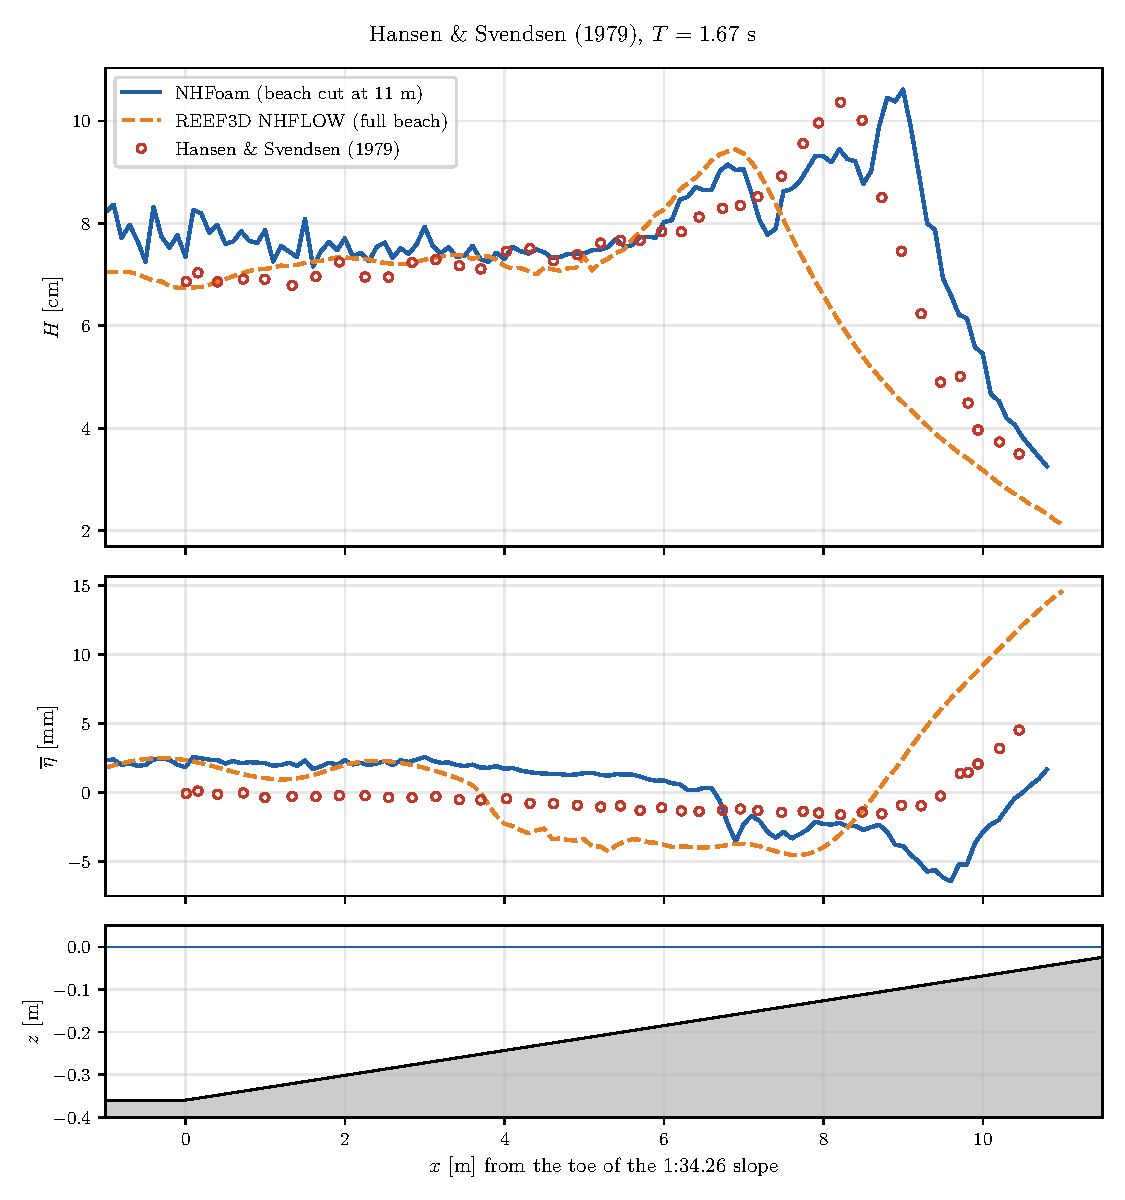
\includegraphics[width=0.85\textwidth]{hansen_svendsen_models.pdf}
\caption{Spilling breakers \citep{hansen1979}: wave height and mean water level.
REEF3D::NHFLOW has the full beach; \NHFOAM\ ends in a shelf with a
velocity-only sponge.}
\label{fig:hs}
\end{figure}

With the interface pressure the incident waves are within a few percent of the
lab at the toe, and the waves break where they did in the flume: the largest
height is 5\% high and 0.1 m from the measured position (the cell layout broke
0.8 m too far inshore). Inside the surf zone, however, the bores lose too
little energy; they keep a sawtooth shape of 7--8 cm down to $x = 10$ m, where
the lab heights have halved. The breaking switch flags about 7 columns at a
time in both layouts, so the onset is right and the dissipation of the
hydrostatic bores is what falls short. REEF3D::NHFLOW, with the full beach and
its own breaking algorithm, breaks too early (largest $H$ 9.4 cm at $x=6.9$ m,
rms 1.5 cm). Without a beach, \NHFOAM\ does not reproduce the mean water level.
NHWAVE is not included: our run of this case (10 layers, $k$--$\epsilon$, full
beach) stopped after 4 s without an error message.

The bore fronts are where the lagged terms of the interface matrix matter
most. With only $A^2$ in the implicit vertical coefficient of
\eqref{eq:midflux}, the pressure correctors diverged under the first steep
bores after 22 s, with a fixed or an adaptive time step alike; the
over-relaxed split fixed it. Bores also need a TVD convection scheme
everywhere: with central differencing away from the breaking columns,
grid-scale oscillations grow behind the bores.

\section{Validation against NHWAVE following \texorpdfstring{\citet{ma2012}}{Ma et al. (2012)}}
\label{sec:ma2012}
\label{sec:ma}

\subsection{Test programme}
\label{sec:ma-programme}

\citet{ma2012} introduced NHWAVE with seven tests (their Section~4), and the
NHWAVE repository ships examples for several of them.
Table~\ref{tab:ma-programme} lists them with what each one tests and whether
\NHFOAM\ can run it today. Tests 1--4 and 6 need no new physics and were run
with both models on the same set-up; tests 5 and 7 need wetting and drying,
which was added afterwards (Section~\ref{sec:wd}), and test 5 and the
surf-zone example are reported there. The NHWAVE runs use the binary built from the
\code{JimKirby/NHWAVE} master branch (Table~\ref{tab:models}); the reruns of
the paper's own tests check that our NHWAVE runs reproduce the published ones.

\begin{table}[ht]
\centering
\caption{The tests of \citet{ma2012} and their status in \NHFOAM.}
\label{tab:ma-programme}
\small
\begin{tabular}{p{0.6cm}p{4.0cm}p{3.6cm}p{2.5cm}p{2.5cm}}
\toprule
 & test & what it tests & reference & \NHFOAM \\
\midrule
4.1 & standing wave in a closed basin, $kD = \pi$, $2\pi$, $3\pi$ & dispersion with 3--10 layers & linear theory & Section~\ref{sec:ma-basin} \\
4.2 & solitary wave, $H/h = 0.5$, constant depth & nonlinearity, time accuracy & exact solution & Section~\ref{sec:ma-solitary} \\
4.3 & periodic waves over a submerged bar & shoaling, release of harmonics & \citet{luth1994} & Section~\ref{sec:ma-bar} \\
4.4 & elliptic shoal on a 1:50 slope & 3D refraction and diffraction & \citet{berkhoff1982} & Section~\ref{sec:ma-berkhoff} \\
4.5 & breaking solitary wave run-up & breaking, wetting and drying & \citet{synolakis1987} & Section~\ref{sec:wd-runup} \\
4.6 & 3D rigid landslide, $d = 61$ mm & moving bottom, short trailing waves & \citet{enet2007} & Section~\ref{sec:ma-landslide} \\
4.7 & longshore current on a plane beach & breaking-driven currents & \citet{visser1991} & Section~\ref{sec:brk-ls} \\
-- & surf zone (NHWAVE example \code{tingkirby}) & breaking, set-up, undertow & \citet{ting1994} & Sections~\ref{sec:wd-tk}, \ref{sec:brk-spill} \\
\bottomrule
\end{tabular}
\end{table}

The tests were run in order of increasing complexity, and each was used to look
for weaknesses of \NHFOAM\ before moving on. Two of them changed the code and
its defaults: the standing waves showed that the TVD convection scheme damps
steep short waves, and the solitary wave showed that the time integration was
only first order for nonlinear waves (Section~\ref{sec:time}). The surf zone
of \citet{ting1994} later led to the breaking eddy viscosity of
Section~\ref{sec:brk}, which is used for test 4.7. The elliptic
shoal showed when the low-dissipation scheme must not be used, and
Section~\ref{sec:ma-summary} collects all the findings.

\FloatBarrier
\subsection{Standing wave in a closed basin}
\label{sec:ma-basin}

A standing wave of amplitude $a = 0.1$ m and wavelength $L = 20$ m, the length of
the closed basin, is started from rest with $\eta = a\cos kx$. The depth is
$D = 10$, 20 or 30 m, so $kD = \pi$, $2\pi$ or $3\pi$, and $\Delta x = 0.2$ m.
\citet{ma2012} report the normalised rms error at $x = 17.5$ m over 30 s,
\begin{equation}
  \epsilon = \frac{1}{H}\sqrt{\overline{(\eta_a - \eta)^2}},\qquad
  \eta_a = a\cos(kx)\cos(\omega t),\quad H = 2a,
  \label{eq:basinerr}
\end{equation}
for 3, 5, 8 and 10 layers. Both models were run with the same layers; NHWAVE
with its adaptive time step (CFL 0.5), \NHFOAM\ with $\Delta t = 5$ ms.

\begin{table}[ht]
\centering
\caption{Standing wave: normalised rms error \eqref{eq:basinerr} [\%] at
$x = 17.5$ m. LLV: \code{limitedLinearV}; FL2: \code{filteredLinear2V 0.2 0}.}
\label{tab:ma-basin}
\small
\begin{tabular}{llcccc}
\toprule
$kD$ & layers & \citet{ma2012} & NHWAVE, rerun & \NHFOAM, LLV & \NHFOAM, FL2 \\
\midrule
$\pi$ & 3 & 1.63 & 1.69 & 0.65 & 0.56 \\
 & 5 & 0.90 & 0.87 & 0.18 & 0.12 \\
 & 8 & 0.61 & 0.67 & 0.09 & 0.07 \\
 & 10 & 0.53 & 0.60 & 0.11 & 0.11 \\
\addlinespace
$2\pi$ & 3 & 3.07 & 3.05 & 1.08 & 0.16 \\
 & 5 & 1.50 & 1.43 & 0.67 & 0.16 \\
 & 8 & 0.81 & 0.80 & 0.33 & 0.17 \\
 & 10 & 0.64 & 0.66 & 0.24 & 0.17 \\
\addlinespace
$3\pi$ & 3 & 4.90 & 4.81 & 1.28 & 0.25 \\
 & 5 & 2.50 & 2.40 & 1.17 & 0.17 \\
 & 8 & 1.35 & 1.24 & 0.68 & 0.17 \\
 & 10 & 1.00 & 0.94 & 0.48 & 0.17 \\
\bottomrule
\end{tabular}
\end{table}

\begin{figure}[ht]
\centering
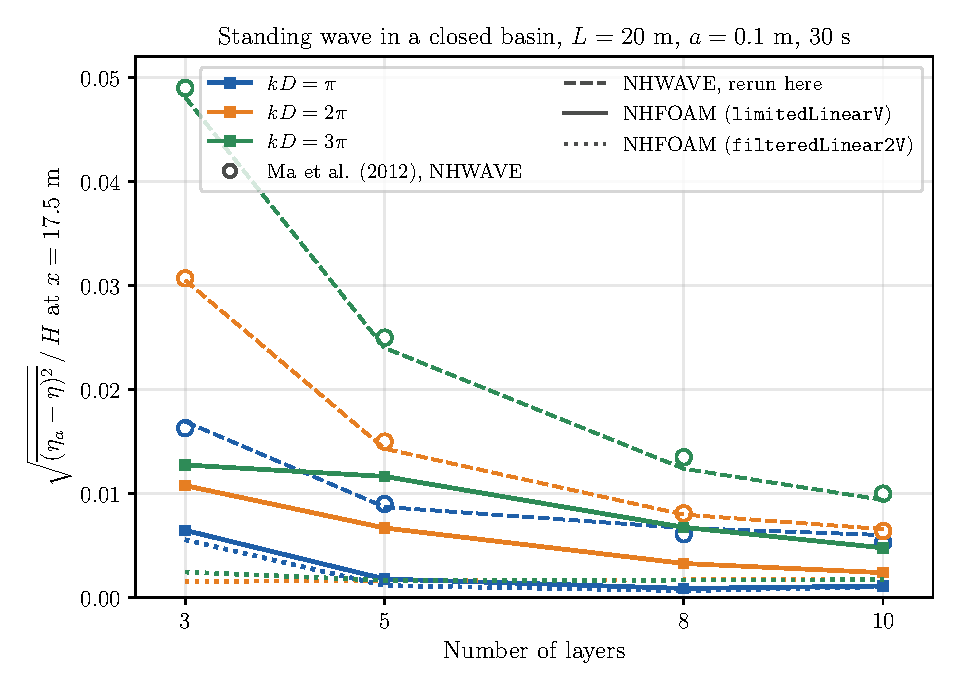
\includegraphics[width=0.8\textwidth]{ma2012_basin.pdf}
\caption{Standing wave in a closed basin: normalised rms error at $x=17.5$ m
against the number of layers. Circles: \citet{ma2012}; dashed: NHWAVE rerun
here; solid and dotted: \NHFOAM\ with the TVD and the filtered central
convection scheme.}
\label{fig:ma-basin}
\end{figure}

Our NHWAVE runs reproduce the published errors to within 0.1 percentage
points (Table~\ref{tab:ma-basin}, Fig.~\ref{fig:ma-basin}), so the NHWAVE
set-up is the paper's. \NHFOAM\ is 2.5--4 times more accurate with the TVD
scheme, and 3--20 times with the filtered central scheme, with which the error
is 0.16--0.25\% for $kD \ge 2\pi$ whatever the number of layers. The remaining
0.56\% at $kD=\pi$ with three layers is the period error of three layers
($-0.07\%$, Section~\ref{sec:dispersion}) accumulated over 8.4 periods.

The difference between the two convection schemes is damping, not phase. The
TVD limiter acts on this wave although its steepness is only $ka = 0.031$: with \code{limitedLinearV} the amplitude at $kD = 3\pi$ with three
layers decays by 8.5\% over 30 s, with \code{filteredLinear2V} by 1.7\%, with
\code{LUST} by 2.8\%. The damping is nonlinear: a wave ten times smaller lost
0.09\%, and halving the time step changed nothing. Repeated with the flux
extrapolation of Section~\ref{sec:time}, the errors of the filtered runs did not
change in the second decimal. This test is the reason
\code{filteredLinear2V} is now recommended for waves that do not break.

\FloatBarrier
\subsection{Solitary wave}
\label{sec:ma-solitary}

A solitary wave of $H/h = 0.5$ travels 150 m over a flat bottom ($h = 1$ m,
$\Delta x = 0.1$ m, 3 layers, 40 s). Its exact shape and velocity field come from
Babenko's equation \citep{babenko1987}, solved with the Petviashvili iteration
\citep{clamond2013} to a residual of $10^{-13}$ (\code{validation/solitary\_exact.py}).
Both models start from the exact $\eta$ and $\bm{u}$; \NHFOAM\ also from the exact
pressure, $\prgh = \tfrac12\left(c^2 - |\bm{u}-c\bm{e}_x|^2\right)$ in the frame
of the wave. NHWAVE runs with CFL 0.5 ($\Delta t \approx 10$ ms), \NHFOAM\ with
$\Delta t = 5$ ms. Table~\ref{tab:ma-solitary} compares the peaks of $\eta$, and of
$u$ and $w$ at mid-depth, with the exact solution after 40 s, and
Fig.~\ref{fig:ma-solitary} shows the profiles.

\begin{table}[ht]
\centering
\caption{Solitary wave, $H/h = 0.5$, 3 layers, $t = 40$ s: error of the peaks of
$\eta$, $u$ and $w$ (mid-depth) and position of the crest relative to the exact
solution. CPU: one core, approximate (runs shared the machine). LLV:
\code{limitedLinearV}; FL2: \code{filteredLinear2V 0.2 0}.}
\label{tab:ma-solitary}
\footnotesize
\begin{tabular}{lccccc}
\toprule
run & $\eta_{\max}$ & $u_{\max}$ & $w_{\max}$ & crest & CPU \\
\midrule
NHWAVE                                            & $-2.3\%$ & $-0.7\%$ & $+0.4\%$ & $-0.08$ m & 570 s \\
\NHFOAM\ before the fix, LLV    & $-6.4\%$ & $-4.3\%$ & $-4.6\%$ & $-0.77$ m & 240 s \\
\quad $2\Delta t$ (10 ms)                         & $-10.3\%$ & $-7.6\%$ & $-9.4\%$ & $-1.37$ m & 110 s \\
\quad $\Delta t/2$ (2.5 ms)                       & $-4.4\%$ & $-2.6\%$ & $-2.2\%$ & $-0.47$ m & 400 s \\
\quad central convection        & $-5.3\%$ & $-3.7\%$ & $-3.5\%$ & $-0.67$ m & 230 s \\
\quad 5 layers                                    & $-5.7\%$ & $-4.2\%$ & $-5.5\%$ & $-0.77$ m & 350 s \\
\quad a non-orthogonal corrector                  & $-6.4\%$ & $-4.4\%$ & $-4.6\%$ & $-0.77$ m & -- \\
\quad 2 outer correctors                          & $-2.3\%$ & $-0.9\%$ & $+0.2\%$ & $-0.17$ m & 390 s \\
\quad 2 outer corr., mesh fixed in the 2nd & $-2.3\%$ & $-0.9\%$ & $+0.2\%$ & $-0.17$ m & 350 s \\
\NHFOAM, flux extrapolation, LLV & $-2.3\%$ & $-0.9\%$ & $+0.3\%$ & $-0.17$ m & 210 s \\
\NHFOAM, flux extrapolation, FL2 & $\bm{-1.0\%}$ & $\bm{-0.2\%}$ & $\bm{+1.6\%}$ & $\bm{-0.07}$ m & 210 s \\
\bottomrule
\end{tabular}
\end{table}

\begin{figure}[ht]
\centering
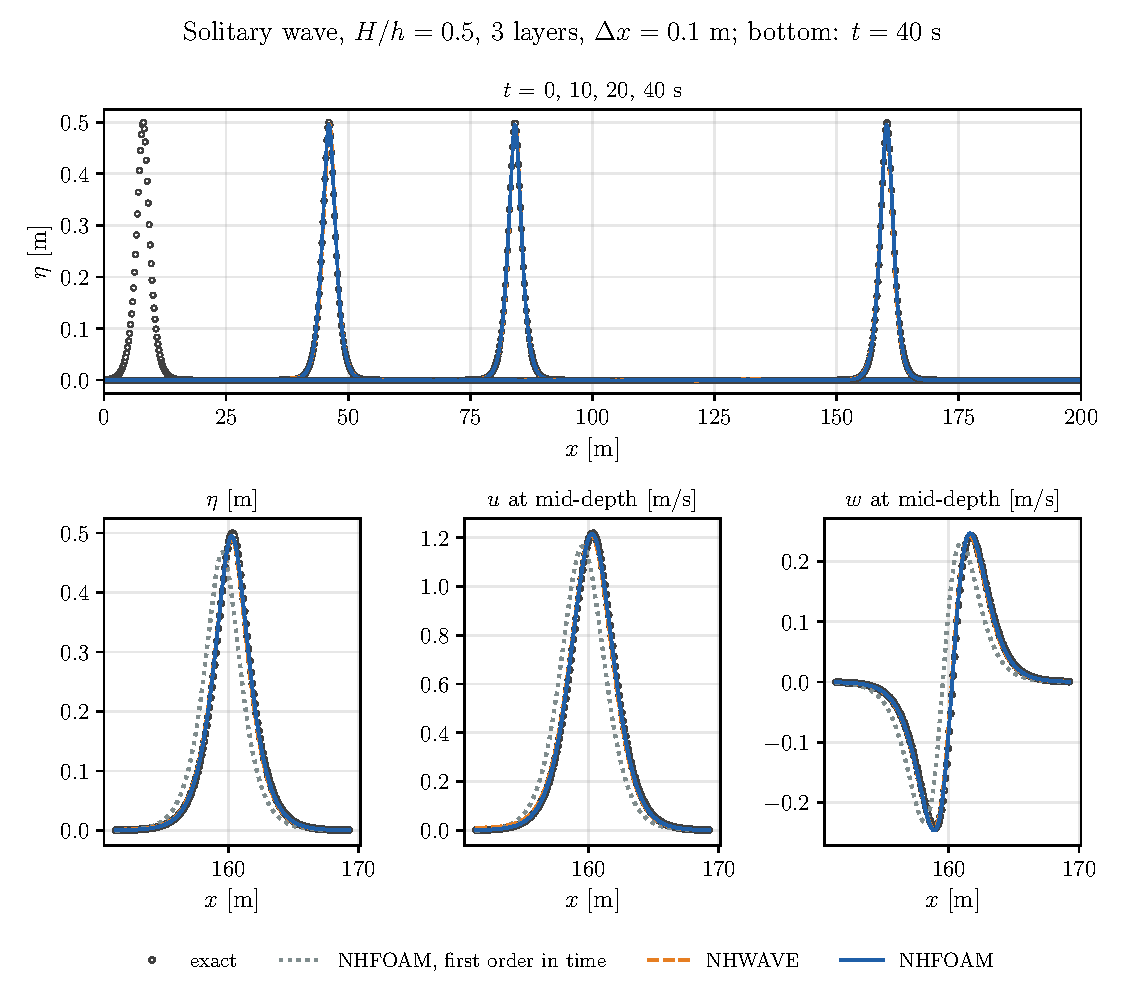
\includegraphics[width=\textwidth]{ma2012_solitary.pdf}
\caption{Solitary wave, $H/h = 0.5$, 3 layers. Top: elevation at $t = 0$, 10, 20
and 40 s. Bottom: $\eta$, $u$ and $w$ at mid-depth around the crest at
$t = 40$ s. \NHFOAM: flux extrapolation and \code{filteredLinear2V}; dotted:
\NHFOAM\ before the fix (one outer corrector, flux of level $n$).}
\label{fig:ma-solitary}
\end{figure}

Before the fix, \NHFOAM\ lost 6.4\% of the wave height in 40 s, three times as
much as NHWAVE, and the crest fell 0.77 m behind. Neither the convection
scheme, the number of layers nor the non-orthogonal correction explained it.
The time step did: the error grew from $-4.4\%$ to $-6.4\%$ and $-10.3\%$ as
$\Delta t$ was doubled twice, i.e.\ linearly in $\Delta t$, and extrapolating
those three runs to $\Delta t\to0$ gives $-2.3\%$ and a lag of 0.17 m. A second
outer corrector gave exactly that, with the mesh moved again in the second
corrector or not. So the cause was not the position of the mesh but the
linearisation of the convection term with the flux of the previous time level
(Section~\ref{sec:time}). Extrapolating the convecting flux \eqref{eq:fluxext}
gives the same result as the second outer corrector at the cost of one, and is
now the default. With it and \code{filteredLinear2V}, the wave keeps its height
after an initial adjustment (about $-1\%$ from $t = 10$ s on) and travels at the
exact speed to within 0.07 m in 150 m. NHWAVE's remaining loss ($-2.3\%$) is the
numerical dissipation of its shock-capturing scheme.

\FloatBarrier
\subsection{Periodic waves over a submerged bar}
\label{sec:ma-bar}

This is NHWAVE's own example (\code{examples/submerged\_bar}), case A of
\citet{luth1994} ($H = 2$ cm, $T = 2.02$ s) with three layers, as in
\citet{ma2012}: a linear boundary wavemaker, a 10 m sponge, $\Delta x = 2$ cm,
CFL 0.5 and, as distributed, a bottom drag coefficient of 0.006. Only the list of
gauges was extended to all ten. \NHFOAM\ runs on the same domain with an 8 m
wave-making zone upstream of NHWAVE's wavemaker, the same sponge, three layers
and $\Delta t = 5$ ms, without bottom friction. Both runs last 40 s and are
compared with the measurements over the last 4 s, with one time shift per run
fitted at $x = 22$ m (Fig.~\ref{fig:ma-bar}, Table~\ref{tab:ma-bar}).

\begin{figure}[p]
\centering
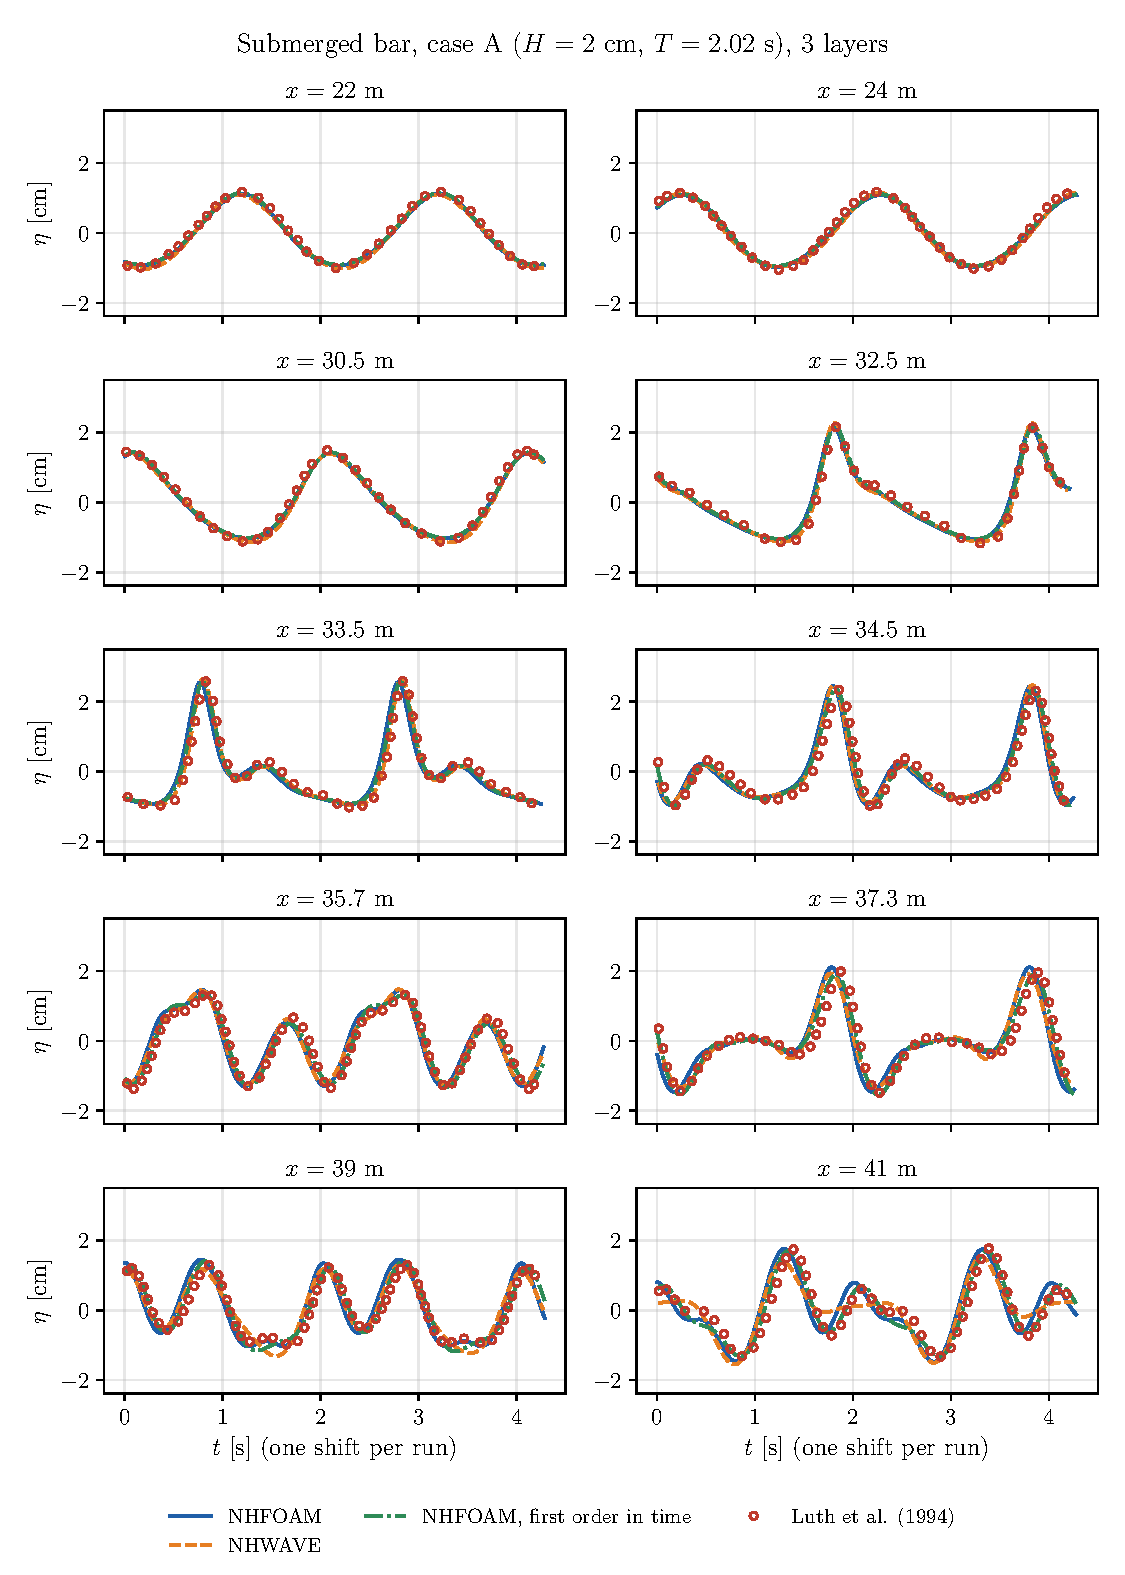
\includegraphics[width=0.9\textwidth]{ma2012_bar.pdf}
\caption{Submerged bar, case A, 3 layers: \NHFOAM\ (flux extrapolation,
\code{filteredLinear2V}), NHWAVE and \NHFOAM\ before the fix of the time
integration, against \citet{luth1994}.}
\label{fig:ma-bar}
\end{figure}

\begin{table}[ht]
\centering
\caption{Submerged bar, case A, 3 layers, window ending at 40 s. Phase: time
shift of the best fit at $x = 35.7$--41 m relative to the shift at $x=22$ m
(negative: the model is early).}
\label{tab:ma-bar}
\small
\begin{tabular}{lccc}
\toprule
 & \NHFOAM & NHWAVE & \NHFOAM\ before the fix \\
\midrule
rms error over the 10 gauges & 0.31 cm & 0.24 cm & 0.16 cm \\
mean $|\Delta H|/H$          & 4.9\%   & 3.8\%   & 4.6\% \\
phase at $x = 35.7$--41 m    & $-0.05$ to $-0.08$ s & $-0.03$ to $-0.08$ s & $-0.01$ to $-0.035$ s \\
\bottomrule
\end{tabular}
\end{table}

Both models reproduce the shoaling on the front slope and the decomposition
into free harmonics behind the bar, with wave heights within a few percent of
the measurements at most gauges. Most of the rms error is phase. After the fix
of the time integration, \NHFOAM's waves over and behind the bar are as early as
NHWAVE's, by up to 0.08 s at the last gauges. Before the fix they were closer to
the measured phase, because the first-order lag slowed them by about 0.5\%, the
same lag that delayed the solitary wave of Section~\ref{sec:ma-solitary}.
With the fix, halving the time step moves the phase by less than 0.005 s, so the
solution is converged in time. The better match of the measured phase before the
fix was therefore a cancellation of errors, and the residual phase error is
shared by both models. Its likely sources are the
linear wave generation, which releases spurious free harmonics, and the long
waves and mean levels of the closed flume (Section~\ref{sec:bar10}). A second
outer corrector, or the TVD instead of the filtered scheme, changes the rms
error by less than 0.02 cm, and the filtered scheme stayed stable over the 40 s
(and over 65 s with ten layers in case C).

\FloatBarrier
\subsection{Elliptic shoal on a sloping bottom}
\label{sec:ma-berkhoff}

The experiment of \citet{berkhoff1982} tests refraction and diffraction in 3D:
an elliptic shoal on a 1:50 slope whose contours are rotated by $20^\circ$
focuses regular waves ($T = 1$ s, $H_0 = 4.64$ cm, $h = 0.45$ m offshore) into a
caustic behind it. The bathymetry is that of \citet{ma2012}, their eqs.\
(49)--(51); it matches the depth file of NHWAVE's example
(\code{examples/berkhoff}) to 2 mm, with the shoal centre at
$(12.025, 10.025)$ m in the coordinates of that example. NHWAVE generates the
waves at its left boundary, absorbs them in a 3 m sponge and has walls at
$y = 0$ and 20 m; \NHFOAM\ has a 3 m wave-making zone upstream of NHWAVE's
wavemaker, the same sponge and walls. To keep the cost of both runs to a few
hours on one core, the grid is twice as coarse as in the paper in both
directions: $\Delta x = 5$ cm and $\Delta y = 10$ cm ($600\times200$ columns),
with three uniform layers (the paper used five). This gives 29 cells per
wavelength offshore and about 18 behind the shoal. NHWAVE runs with CFL 0.5
and, as distributed, a bottom drag coefficient of 0.006; \NHFOAM\ with
$\Delta t = 10$ ms ($T/100$), flux extrapolation and \code{filteredLinear2V}.
Both runs last 30 s, and the wave height is the mean of max $-$ min over the
last five periods at 174 points along the eight measurement sections
(sections 1--5 across the flume at $x = 1$, 3, 5, 7, 9 m behind the shoal
centre, sections 6--8 along it at $y = -2$, 0, 2 m).

Because \NHFOAM\ generates the waves inside a zone and ramps them up over two
periods, its wave train reaches the shoal 2.25 s after NHWAVE's (measured from
the arrival of half the final height at section 1, the same at all its points
to within 0.2 s). Its wave heights are therefore taken over the five periods
ending at $t = 32.25$ s, the same stage of the wave train as NHWAVE's last five
periods ending at 30 s. Figure~\ref{fig:ma-berkhoff} shows the wave heights,
and Table~\ref{tab:ma-berkhoff} the normalised rms error per section,
$\sqrt{\overline{(H_{\mathrm{mod}}-H_{\mathrm{obs}})^2}}\,/\,\overline{H_{\mathrm{obs}}}$,
as defined by \citet{ma2012}.

\begin{figure}[p]
\centering
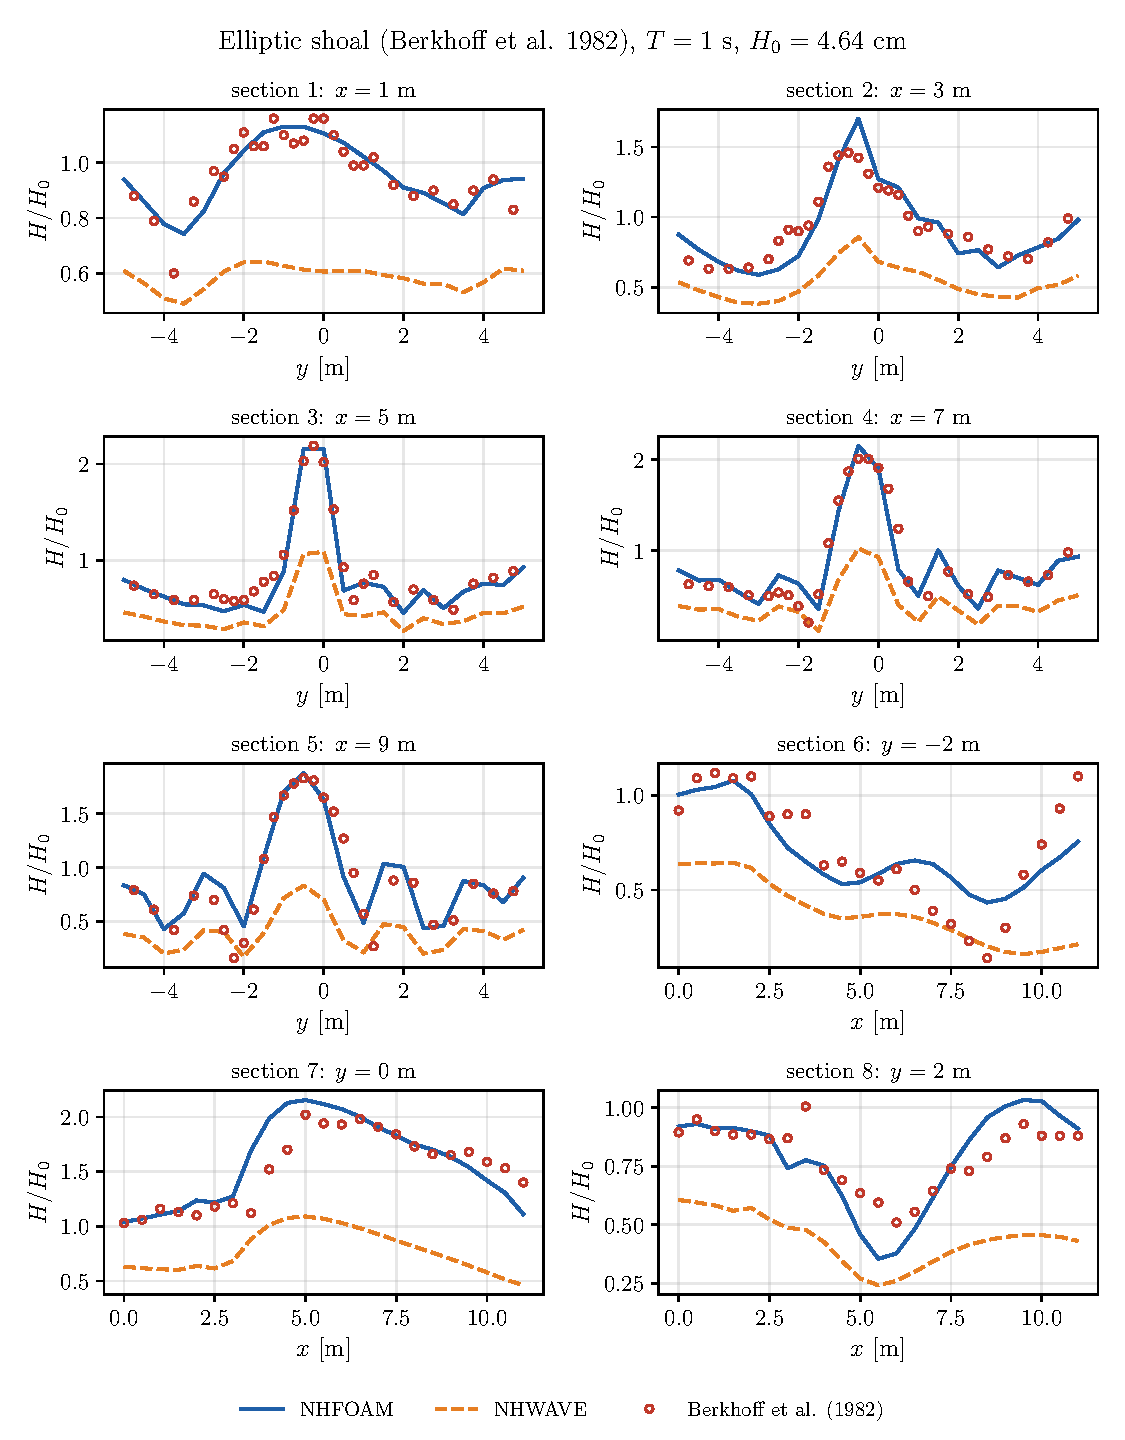
\includegraphics[width=\textwidth]{ma2012_berkhoff.pdf}
\caption{Elliptic shoal: wave height along the eight measurement sections.
\NHFOAM\ and NHWAVE on the same grid ($\Delta x = 5$ cm, $\Delta y = 10$ cm,
3 layers) against \citet{berkhoff1982}.}
\label{fig:ma-berkhoff}
\end{figure}

\begin{table}[ht]
\centering
\caption{Elliptic shoal: normalised rms error of the wave height per
section. \citet{ma2012}: NHWAVE on a grid twice as fine in $x$ and $y$ with five
layers (the paper gives sections 1, 3 and 5 only).}
\label{tab:ma-berkhoff}
\small
\setlength{\tabcolsep}{3.8pt}
\begin{tabular}{lccccccccc}
\toprule
section & 1 & 2 & 3 & 4 & 5 & 6 & 7 & 8 & mean \\
\midrule
\NHFOAM, $\Delta x = 5$ cm         & 0.06 & 0.12 & 0.13 & 0.18 & 0.21 & 0.24 & 0.14 & 0.14 & 0.15 \\
NHWAVE, $\Delta x = 5$ cm          & 0.41 & 0.45 & 0.54 & 0.62 & 0.67 & 0.56 & 0.52 & 0.46 & 0.53 \\
NHWAVE, $\Delta x = 2.5$ cm \citep{ma2012} & 0.07 & -- & 0.11 & -- & 0.11 & -- & -- & -- & -- \\
\bottomrule
\end{tabular}
\end{table}

On this grid \NHFOAM\ reproduces the focusing behind the shoal: the peak of
2.1--2.2 $H_0$ at sections 3 and 4, the side lobes, and the decay along
section 7. At sections 1 and 3 its errors (0.06 and 0.13) are close to those
of NHWAVE on the fine grid of the paper (0.07 and 0.11). NHWAVE on the coarse
grid has the right pattern but only about 60\% of the measured heights: its
incident waves lose 30\% of their height over the first 10 m (from 42.7 mm at
$x = 1$ m to 30.1 mm at $x = 11$ m at $t = 30$ s, along $y = 5$ m), while
\NHFOAM's lose 5\% (46.5 to 44.1 mm, partly by refraction). At 29 cells per
wavelength the shock-capturing scheme of NHWAVE is too dissipative, and it
needs the paper's grid. \NHFOAM\ comes close to the paper's accuracy at
sections 1 and 3 with a quarter of the columns; at section 5 its error is twice
the paper's (0.21 against 0.11). The errors at sections 1--3 change by less than
0.02 when the window is moved by $\pm1$ s, those at sections 4--8, farther from
the wave-maker, by up to 0.08: there the wave train is not yet fully established
by $t\approx 32$ s (in NHWAVE, by 30 s), and a longer run would be needed.

The \NHFOAM\ run itself failed at $t\approx35$ s, after the analysis window
and outside the measurement area. In the shallow corner of the domain at the
south wall, where the depth reaches its minimum of 0.07 m from $x\approx22.7$ m
on, the shoaled waves reach $H/h \approx 1$ and break, and the filtered central
scheme without a breaking model cannot carry the resulting bores
(Section~\ref{sec:convection}). Restarted from $t = 30$ s with
\code{limitedLinearV} and the hydrostatic front approximation, the run went on
to 37 s with up to 171 breaking columns in that corner. The mean error over the
sections at the window ending at 34.5 s was the same for both runs (0.17), and
it fell to 0.14 by 37 s as the wave train at the far sections became
established. A domain in which waves break anywhere, even outside the region of
interest, therefore needs the TVD scheme and the breaking model.

\FloatBarrier
\subsection{3D rigid landslide}
\label{sec:ma-landslide}

\citet{ma2012} used the $d = 61$ mm case of \citet{enet2007}, which was already
compared in Section~\ref{sec:seabed}. It was rerun with the fixed time
integration and \code{filteredLinear2V}, on the same mesh (5 layers,
$\Delta x = \Delta y = 2.5$ cm, the domain ending in a wall 0.2 m from the
shoreline) and against the same NHWAVE run (3 layers, $\Delta x = 2$ cm, full
beach). Figure~\ref{fig:ma-landslide} and Table~\ref{tab:ma-landslide} show the
result.

\begin{figure}[ht]
\centering
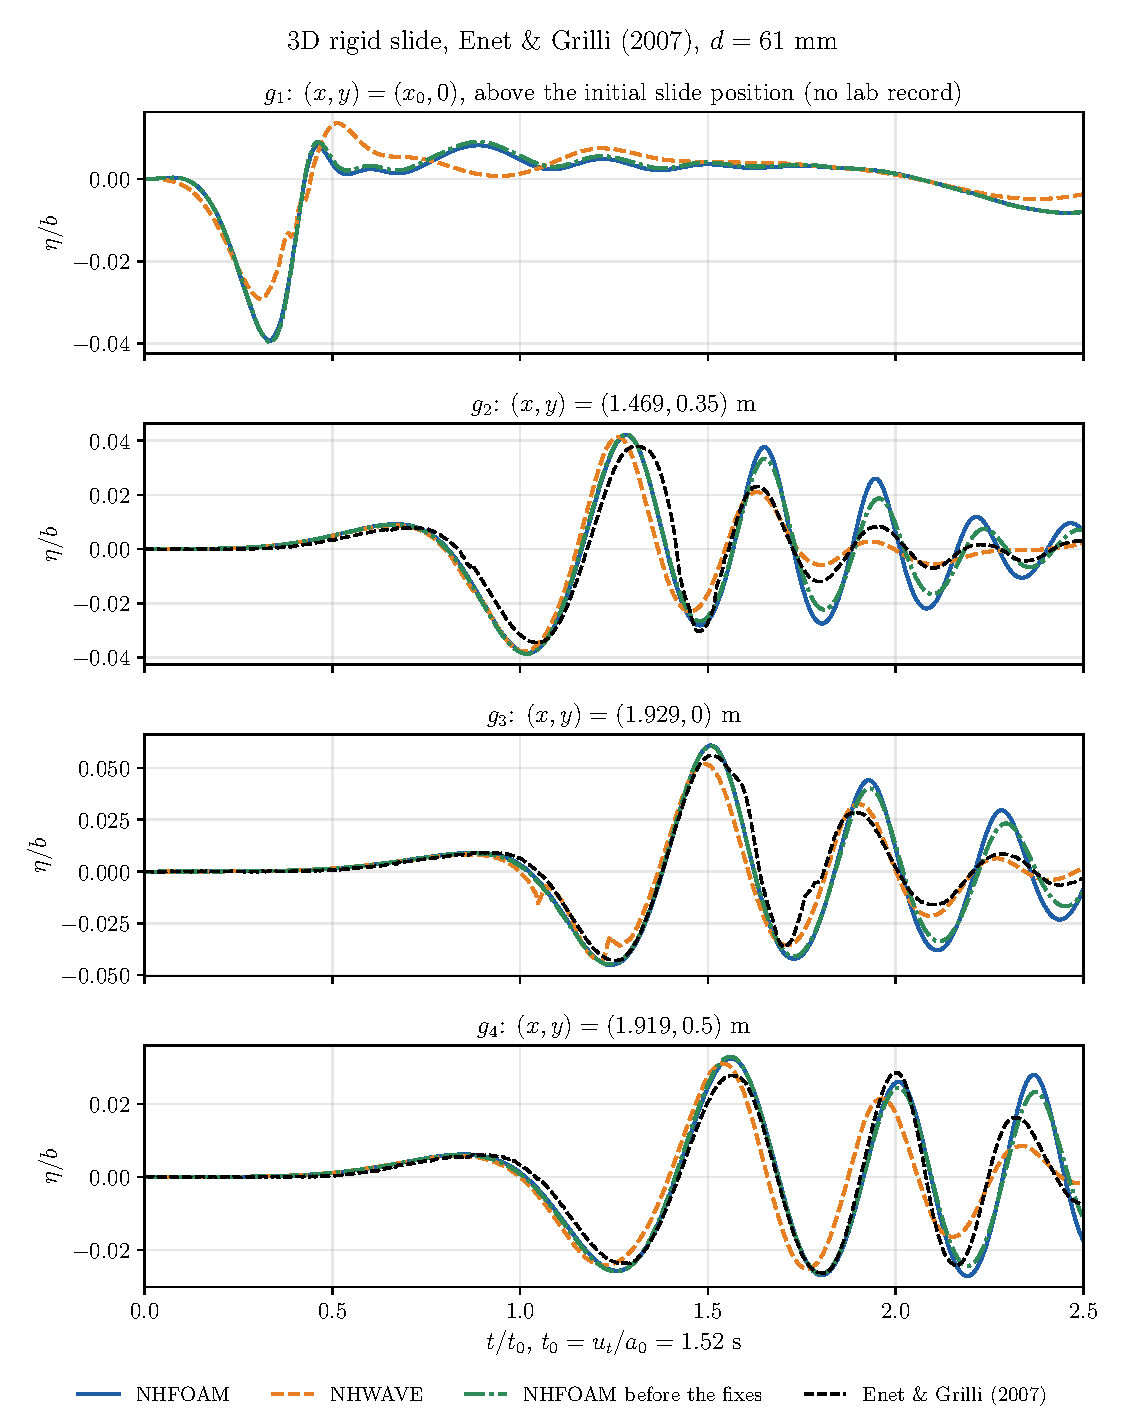
\includegraphics[width=0.85\textwidth]{ma2012_landslide.pdf}
\caption{3D rigid landslide, $d = 61$ mm: \NHFOAM\ with the fixes, NHWAVE and
\NHFOAM\ before the fixes, against \citet{enet2007}.}
\label{fig:ma-landslide}
\end{figure}

\begin{table}[ht]
\centering
\caption{3D rigid landslide, $d = 61$ mm: the largest crest and the two crests
after it [mm] (maxima between zero up-crossings, $t < 2.5\,t_0$).}
\label{tab:ma-landslide}
\small
\begin{tabular}{lccc}
\toprule
 & g2 (1.469, 0.35) & g3 (1.929, 0) & g4 (1.919, 0.5) \\
\midrule
lab                       & 15.0, 9.1, 3.3  & 22.2, 11.3, 3.5 & 11.3, 6.4, -- \\
\NHFOAM                   & 16.7, 14.9, 10.3 & 24.1, 17.4, 11.7 & 12.8, 10.3, 11.1 \\
\NHFOAM\ before the fixes & 16.7, 13.2, 7.4  & 23.9, 15.9, 9.2  & 13.0, 9.7, 9.2 \\
NHWAVE                    & 16.3, 8.3, 1.1   & 20.5, 12.9, 2.5  & 12.3, 8.5, 3.4 \\
\bottomrule
\end{tabular}
\end{table}

The leading trough and crest change by less than 2\%: they are long waves,
and the time integration and the convection scheme hardly affect them. The
trailing waves were too large before the fixes, and they are 10--25\% larger
now that the numerical damping is smaller: the second crest is 1.5 times the
measured one and the third about three times, while NHWAVE follows the measured
decay. The excess is therefore not numerical damping that \NHFOAM\ lacks; its
likely cause is the wall that replaces the beach 0.2 m from the shoreline. The
slide also sends waves towards the shore. In \NHFOAM\ they are reflected by
the wall, less than 0.4 m shoreward of the slide, and come back to the gauges at
about $t \approx 1.5\,t_0$, when the excess starts; on NHWAVE's beach they run
up and are partly dissipated. This test
needs the beach to be conclusive; with the wetting and drying of
Section~\ref{sec:wd} it can now be rerun with it.

\paragraph{With the beach.} The run was repeated with the slope continued
0.25 m inland of the still-water shoreline (the bed 6.7 cm above the still
water) and wetting and drying (5 mm film), otherwise unchanged (147\,600
cells; Fig.~\ref{fig:ma-landslide-beach}). The leading trough and crest
change by less than 4\%, and the trailing waves are no smaller: the
largest crest and the two after it are 17.3, 15.7 and 10.7 mm at g2
(wall: 16.7, 14.9, 10.3), 23.4, 18.2 and 11.3 mm at g3 (24.1, 17.4, 11.7)
and 12.7, 11.6 and 10.7 mm at g4 (12.8, 10.3, 11.1). The wall is therefore
not the cause of the excess. The trailing waves ($kh = 3$--5) follow the
convection scheme instead: they were smaller with the more dissipative TVD
scheme before the fixes, and NHWAVE's shock-capturing scheme damps them
most. Whether the measured decay of the trailing waves is physical damping
that an inviscid model lacks, or comes from details of the slide motion,
remains open.

\begin{figure}[!htbp]
\centering
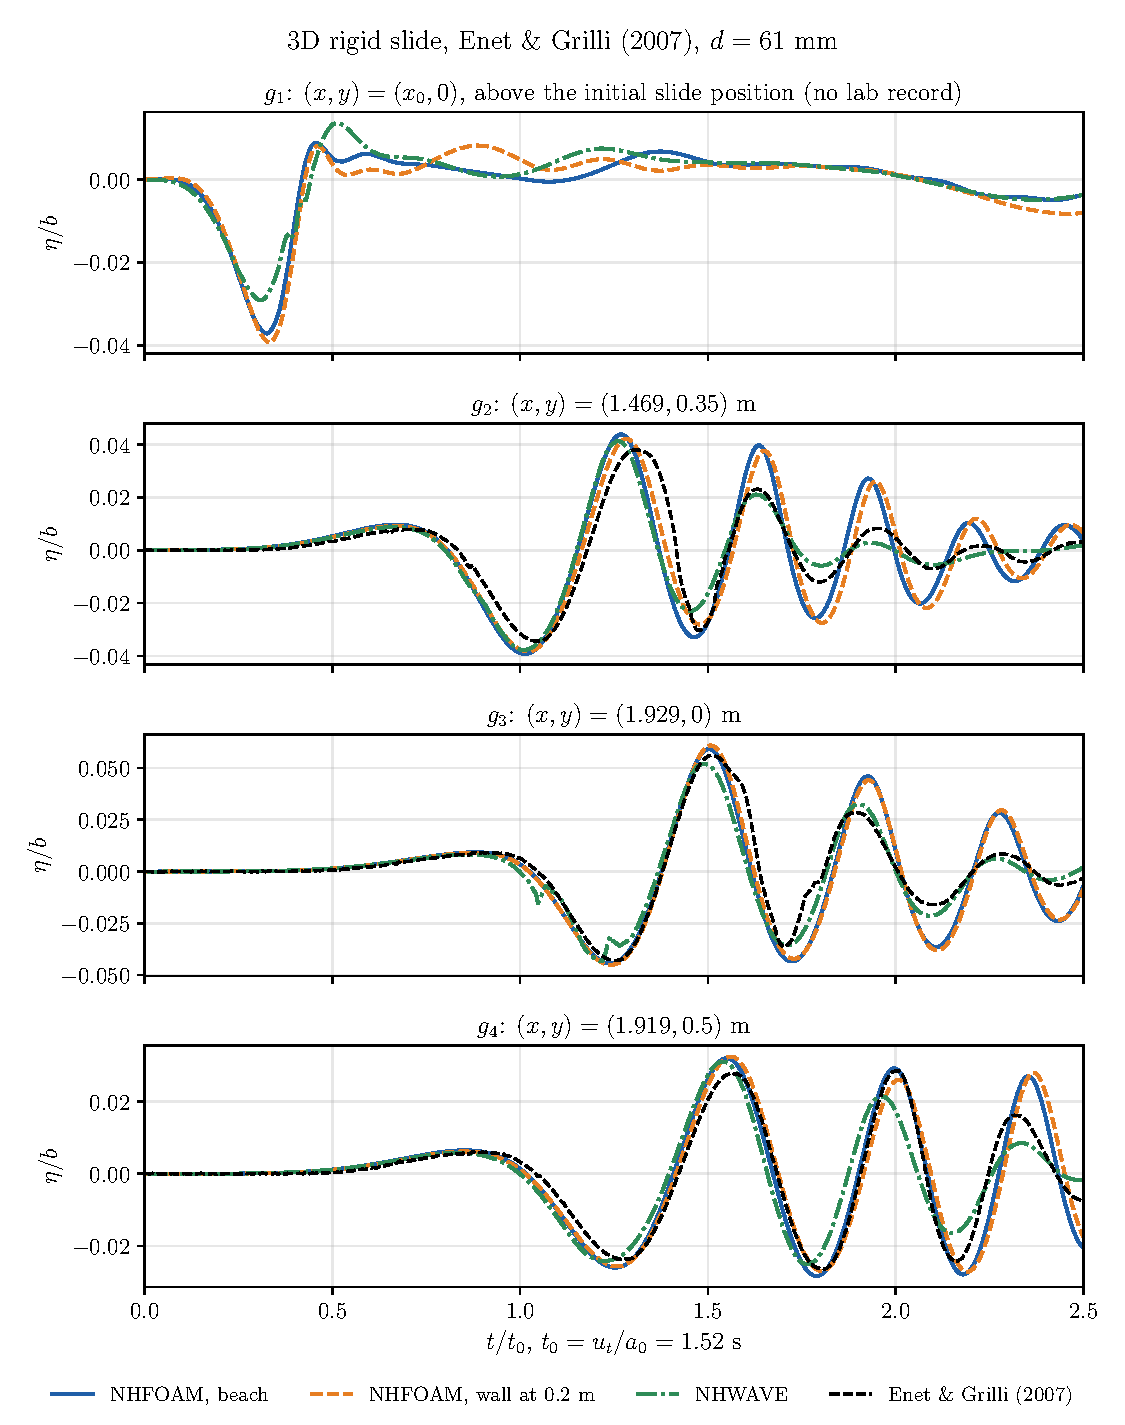
\includegraphics[width=0.85\textwidth]{landslide_beach.pdf}
\caption{3D rigid landslide, $d = 61$ mm: \NHFOAM\ with the beach and
wetting and drying, with the wall 0.2 m from the shoreline, and NHWAVE,
against \citet{enet2007}.}
\label{fig:ma-landslide-beach}
\end{figure}

\FloatBarrier
\subsection{Summary of the problems found and their fixes}
\label{sec:ma-summary}

Table~\ref{tab:fixes} lists the weaknesses that the comparisons with NHWAVE
exposed, here and in Section~\ref{sec:verification}, with their causes and
fixes.

\begin{table}[ht]
\centering
\caption{Problems found by the tests and their fixes.}
\label{tab:fixes}
\small
\begin{tabular}{p{2.3cm}p{3.6cm}p{3.6cm}p{4.6cm}}
\toprule
test & problem & cause & fix and effect \\
\midrule
dispersion (Section~\ref{sec:dispersion}) & 10--20 layers needed for $kh = 4$--7 & cell-centred pressure & pressure on the layer interfaces: 2 layers for $kh \le 7$ \\
3D landslide (Section~\ref{sec:seabed}) & DIC breaks down with thick layers & matrix not diagonally dominant & \code{sigmaColumn} line preconditioner \\
breaking (Section~\ref{sec:breaking}) & pressure correctors diverge under bores & lagged vertical pressure difference through sloping mid-planes & over-relaxed split \eqref{eq:midflux} \\
standing wave (Section~\ref{sec:ma-basin}) & short steep waves damped (8.5\% in 30 s) & TVD limiter & \code{filteredLinear2V} for non-breaking waves: error 0.16--0.25\% for $kD\ge2\pi$ \\
solitary wave (Section~\ref{sec:ma-solitary}) & height $-6.4\%$, crest 0.77 m late in 150 m & convecting flux of level $n$: first order in time & flux extrapolation \eqref{eq:fluxext}: $-1.0\%$, 0.07 m, no extra cost \\
submerged bar (Section~\ref{sec:ma-bar}) & phase closer to the lab before the fix & the first-order lag cancelled an error shared with NHWAVE & none yet; the phase now agrees with NHWAVE \\
submerged bar, long runs (Section~\ref{sec:bar-bc}) & phase drifts by 0.21 s in 20 s & no return current in the wave-making zone & return current (default), or the boundary wavemaker: no drift, steady 1.0 cm error \\
elliptic shoal (Section~\ref{sec:ma-berkhoff}) & run fails at 35 s in a shallow corner & waves break there; filtered scheme, no breaking model & \code{limitedLinearV} and HFA wherever waves break: the run goes on, same errors \\
landslide (Section~\ref{sec:ma-landslide}) & trailing waves 1.5--3 times too large & not the wall: the run with the beach gives the same & open \\
run-up (Section~\ref{sec:wd-runup}) & front too slow, $R/d = 0.41$; oscillating swash & centred face depth, interpolated flux at the tip & upwind (TVD) face depth, supercritical upwind flux: $R/d = 0.531$ (NHWAVE 0.512) \\
surf zone (Section~\ref{sec:wd-tk}) & heights 6 cm too large at $x = 8$ m & too little dissipation behind the hydrostatic front & breaking age and eddy viscosity (Section~\ref{sec:brk}): mean surf-zone error $+6.1 \to +3.5$ cm (NHWAVE $+4.8$) \\
longshore current (Section~\ref{sec:brk-ls}) & breaking region crept into deep water along oblique crests & columns joined at the aged threshold & join at $\beta\sqrt{gD}$ \\
\bottomrule
\end{tabular}
\end{table}

\section{Wetting and drying}
\label{sec:wd}

Tests 4.5 and 4.7 of \citet{ma2012} and the surf-zone example of the NHWAVE
repository need moving shorelines. This section describes the wetting and
drying of \NHFOAM, which follows NHWAVE's mask and thin film
\citep[][Section~3.4]{ma2012} but had to be adapted to the implicit free
surface and the collocated mesh, compares the two treatments, and tests them:
still water against a dry beach, the oscillation in a parabolic basin of
\citet{thacker1981} and a dam break on a dry bed (verification), and the
run-up of a breaking solitary wave \citep{synolakis1987}, the solitary waves
on a conical island of \citet{briggs1995}, the tsunami run-up in the Monai
valley \citep{matsuyama2001}, also on meshes refined around the valley, and
the spilling breakers of \citet{ting1994} (validation, with NHWAVE).

\subsection{Method}
\label{sec:wd-method}

\paragraph{Mask.} A dry column keeps a film of depth $D_{\min}$
(\code{minDepth}), so $\eta = z_b + D_{\min}$. The mask is updated at the start
of every time step from $\eta^n$, with NHWAVE's rules: a dry column floods when
a wet neighbour has a higher surface and more than the film,
$\eta_w > \eta_d$ and $D_w - D_{\min} > \epsilon$; a wet column dries when
$D - D_{\min} \le \epsilon$ ($\epsilon = 10^{-6}$ m), and its surface is then
reset to the film. A column that changes state starts from the film at both
stored time levels, so the BDF2 time derivative sees no jump. A side face is
open when the columns on both sides are wet. A closed face carries no flux and
has no coefficients in the pressure matrix, and in the cell-centred pressure
gradient it acts as a wall: each side sees its own pressure, so a dry
neighbour exerts no force and still water stays at rest against a dry beach.
The velocity of dry columns is held at zero by an implicit sink,
$10^4/\Delta t$ on the diagonal of the momentum equation. The same is done in
a wet column whose side faces are all closed (a puddle left on the beach): its
velocity could only carry it away from the lower neighbour it floods next.

\paragraph{Positivity.} The implicit pressure solve can draw more water from
a shallow column than it holds. After the solve, the side outflows of a column
are limited so that its surface stays at or above the film at the new level:
with the free-surface update of \eqref{eq:bdf2}, the net side outflow may not
exceed
\begin{equation}
  Q_{\max} = -\phi_{\mathrm{bottom}} - \frac{A_h}{a}\left(\eta_{\min} - \hat\eta\right),
  \qquad \eta_{\min} = z_b + D_{\min},
\end{equation}
(relaxation-zone terms included in the code). The outflows of a column that
would exceed it are scaled down by a common factor; this lowers the inflow of
its neighbours, so the sweep is repeated until no column exceeds its limit.
Inflows are never changed by a column's own limit and each face keeps one
value, so volume is conserved to round-off. The only loss is the reset of a
drying column, at most $\epsilon$ per column.

\paragraph{Water depth at the side faces.} The mesh face between two columns
has the depth of the vertical point lines at the column edge, about the mean
of the two columns. With this centred depth the first version of the method
moved flood fronts too slowly and let bores in thin water oscillate: a dam
break on a dry bed advanced at 0.9 m/s where NHWAVE gives 1.25 m/s
(Section~\ref{sec:wd-dambreak}), and the solitary wave of
Section~\ref{sec:wd-runup} ran up to $R/d = 0.41$ instead of 0.51. As in the
semi-implicit schemes of \citet{stelling2003b} and SWASH, the side fluxes now
carry the water depth on the upwind side,
\begin{equation}
  D_f = \eta_f - z_{b,f},\qquad
  \eta_f = \eta_C + \tfrac12\,\psi(r)\,(\eta_D - \eta_C),\qquad
  r = \frac{2\,\bm{d}\cdot\nabla\eta_C}{\eta_D - \eta_C} - 1,
  \label{eq:facedepth}
\end{equation}
where $C$ is the upwind and $D$ the downwind column, $\bm{d}$ the vector
between their centres, $z_{b,f}$ the bottom of the face and $\psi$ a TVD
limiter (van Leer by default; minmod, MC, or $\psi=0$ for the first-order
upwind depth, can be chosen). Next to a column with less than two films of
water the surface ends, and the upwind value is used. All layer fluxes of the
face are scaled by $f = D_f/D_{\mathrm{mesh}}$: in the predicted flux
$\phi_{\mathrm{HbyA}}$, in the implicit coefficients of the pressure matrix and
in the convecting flux of the momentum equation. The face velocity
$\bm{u}_f$, which carries the flux of a time step to the next one (the
$\partial\bm{u}/\partial t$ flux correction and the flux extrapolation of
Section~\ref{sec:time}), stays the flux divided by $f$, so it is not scaled
twice. NHWAVE gets the same upwinding from its MUSCL reconstruction and HLL
fluxes.

\paragraph{Supercritical faces.} Where the upwind column is supercritical,
with a depth-averaged velocity normal to the face above
$\mathrm{Fr}_c\sqrt{gD}$ (\code{upwindFroude}, default 1), the predicted flux of
the face is that of the upwind cell, $\bm{H}_C\cdot\bm{S}_f$, instead of the
interpolated one. An HLL flux does the same once both wave speeds have the
sign of the flow. Without it, the face at the tip of a run-up carries the mean
of a fast and a slow (or resting) column. The switch must stay sharp. When the
upwind flux was blended in below $\mathrm{Fr} = 1$, grid-scale oscillations
grew in the subcritical part of a dam break: the interpolated flux is what
couples pressure and velocity on the collocated mesh, and upwinding it at all
faces next to shallow water made the solution noisy everywhere. A blend
between $\mathrm{Fr} = 1$ and 1.5 lowered the run-up by 10\%.

\paragraph{Faces opened by flooding.} In the step after a column floods, the
predicted flux of the faces it opened may only run into it, since its film
cannot feed the flow. Where it lies lower than the wet column, the face
velocity is at least that of a dam break from rest at the dam,
$\tfrac23\sqrt{g(D_w - D_{\min})}$. Without these two rules a puddle flooded its
lower neighbour every other step without water flowing into it (the flux was
cut to zero by the positivity limiter, and the neighbour dried again); applied
up the slope as well, the dam-break velocity made a film creep up the whole
beach.

\paragraph{Options.} \code{hydrostaticDepth} switches the non-hydrostatic
pressure off in columns shallower than the given depth (as the breaking
columns of Section~\ref{sec:numhfa}). \code{bottomFriction} adds the quadratic
stress $\bm{\tau}_b/\rho = C_d\,|\bm{u}_b|\,\bm{u}_b$ on the bottom cells,
with a constant $C_d$ or $C_d = g n^2/D^{1/3}$ from a Manning coefficient $n$
(it can be used without wetting and drying). The wetting and drying needs the
interface pressure layout. The highest wet bed and the highest surface on land
are written every step to \code{postProcessing/wettingDrying}.

\paragraph{Nonlinear waves.} For the surf-zone test the relaxation zones were
given a second target, the stream-function wave of \citet{fenton1988}: a
Fourier series of order $N$ for $\eta$ and for the stream function, whose
coefficients are computed beforehand (\code{validation/stream\_function.py},
zero mass flux by default, i.e.\ with the return current of a closed flume).
In a flat flume, $h = 0.4$ m, 10 layers and $\Delta x = 2.5$ cm, the zone made
the wave of \citet{ting1994} ($H = 0.125$ m, $T = 2$ s, Ursell number 27)
with $H = 0.1246$--$0.1249$ m at six gauges over 10 m, crest and trough
within 1.4 and 1.1 mm of the theory, and no beating of free harmonics.

\subsection{Comparison with NHWAVE}
\label{sec:wd-nhwave}

Table~\ref{tab:wd-features} sets the two treatments side by side; the NHWAVE
column is read from the source (\code{update\_mask}, \code{construction},
\code{flux\_bc} and \code{eval\_duvw} in \code{nhwave.F}). The mask and the
closed faces are the same. The differences come from the time integration.
NHWAVE updates the depth explicitly from Riemann fluxes, so positivity is a
clip and the upwinding of depth and velocity is built into the HLL flux.
\NHFOAM's surface is implicit, so the outflows must be limited after the
solve, and the upwinding has to be added to the depth and to the predicted
flux explicitly.

\begin{table}[ht]
\centering
\caption{Wetting and drying in NHWAVE and \NHFOAM.}
\label{tab:wd-features}
\small
\begin{tabular}{p{3.0cm}p{5.6cm}p{5.6cm}}
\toprule
 & NHWAVE & \NHFOAM \\
\midrule
mask & from $\eta^n$ at each step: flood if a wet neighbour is higher and has more than the film; dry at the film & same \\
dry cells & $D = D_{\min}$, not updated & $\eta = z_b+D_{\min}$, velocity held at zero \\
faces of dry cells & no mass flux; momentum flux is the wet side's hydrostatic pressure (a wall) & closed: no flux, a wall for the pressure gradient \\
positivity & $D = \max(D, D_{\min})$ after each stage (adds water) & limiter on the outflows (conservative) \\
depth at wet faces & MUSCL (van Leer) reconstruction of $\eta$, HLL flux & TVD (van Leer) reconstruction of $\eta$, upwind next to near-dry columns \\
supercritical faces & HLL takes the upwind flux & predicted flux of the upwind cell \\
newly wet faces & HLL depth diffusion, $\sim c\,\Delta D/2$ & flux only into the new column; dam-break velocity downhill \\
puddles & spread by the HLL diffusion & held at rest until they flood a lower neighbour \\
$q$ in thin water & solved everywhere, no correction in dry cells & solved everywhere; optional $q = 0$ below a depth \\
breaking & shock capturing ($k$--$\epsilon$ in the surf-zone example) & hydrostatic front approximation \\
volume & not conserved exactly (clip) & conserved; a drying column loses $\le\epsilon$ \\
\bottomrule
\end{tabular}
\end{table}

\subsection{Still water and the parabolic basin}
\label{sec:wd-thacker}

Still water against a dry 1:20 beach (film 5 mm, $\Delta x = 5$ cm, 3 layers)
stays at rest: after 10 s the largest velocity is $5\times10^{-9}$ m/s and the
surface deviates by $3\times10^{-10}$ m.

In the parabolic basin $z_b = h_0\,[(x-L/2)^2/a^2 - 1]$ of \citet{thacker1981},
the surface stays planar and oscillates with the period
$T = 2\pi a/\sqrt{2gh_0}$, and both shorelines move by $\pm a\beta$, with
$\beta = B/(a\omega)$. With $a = 100$ m, $h_0 = 0.5$ m, $B = 0.5$ m/s
($T = 200.6$ s), the basin was approximated by 80 straight segments, with
$\Delta x = 1$ m, 3 layers, $\Delta t = 0.25$ s and a 1 mm film
(Fig.~\ref{fig:wd-thacker}). Over two periods the rms error of the surface is
0.3--1.5 mm (0.9 mm overall) and the largest error 7.4 mm, for a surface that
moves by $\pm0.16$ m at the shorelines. The shorelines, taken as the centre of
the last wet column, are within 1.7 m of the exact ones (0.8 m on average, for
$\Delta x = 1$ m), with no drift from the first to the second period.

\begin{figure}[ht]
\centering
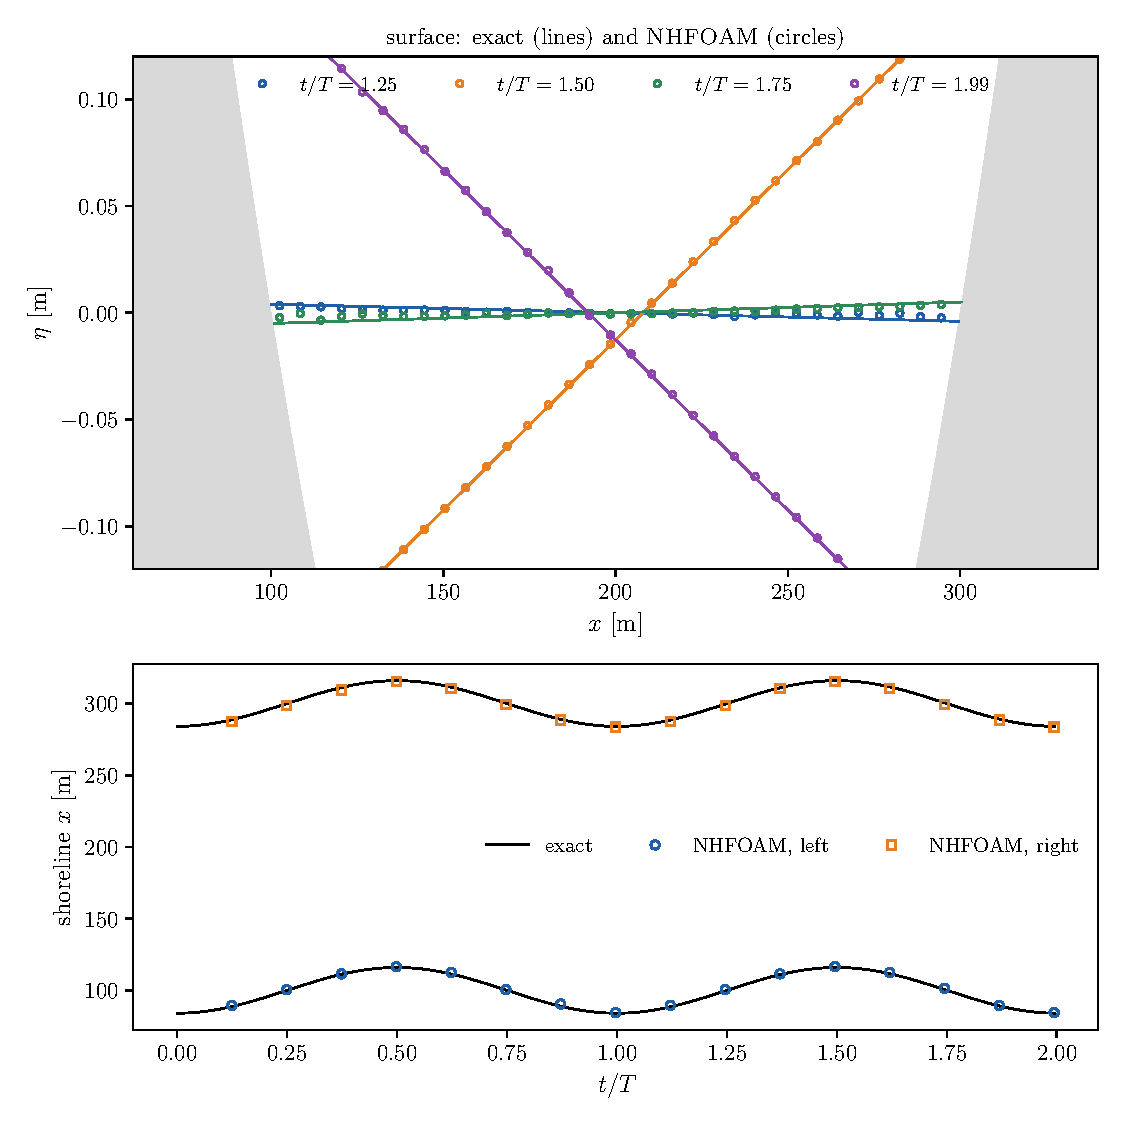
\includegraphics[width=0.85\textwidth]{wd_thacker.pdf}
\caption{Parabolic basin of \citet{thacker1981}: surface at four times of the
second period and the two shorelines over two periods.}
\label{fig:wd-thacker}
\end{figure}

A narrow cell at the shoreline is a hard case. In an earlier mesh, the point
where the depth equals the film was a block vertex, which left a column of
0.1 m among columns of 1 m. With the TVD depth, that column kept a puddle,
because its gradient, taken from its one open face, made the reconstruction
of \eqref{eq:facedepth} reach the dry downwind level. The upwind depth next to
near-dry columns removed the puddle. The errors on that mesh are still four
times larger (rms 3 mm), and the validation meshes avoid such cells.

\subsection{Dam break on a dry bed}
\label{sec:wd-dambreak}

Water of depth $h_0 = 0.1$ m is released at $x = 5$ m onto a dry, flat,
frictionless bed ($\Delta x = 2$ cm, 3 layers, $\Delta t = 4$ ms, film 1 mm,
hydrostatic). \citet{ritter1892}'s solution has a front that runs at
$2\sqrt{gh_0} = 1.98$ m/s with vanishing depth. Neither model gets near it
(Fig.~\ref{fig:wd-dambreak}): both treat the film of the dry columns as water
at rest, which the flow has to push, and both follow the solution of
\citet{stoker1957} for a wet bed as deep as the film, a bore of 1.7 cm moving
at 1.23 m/s. The fronts at $t = 1$, 2 and 3 s are at 6.21, 7.59 and 8.95 m in
\NHFOAM, 6.27, 7.53 and 8.77 m in NHWAVE (MinDep 1 mm) and 6.23, 7.47 and
8.70 m in Stoker's solution. With the centred face depth the front of
\NHFOAM\ moved at 0.9 m/s, behind a pile-up of water at the tip. The film
therefore sets a lower limit to the depth of the flows that a run-up
computation can resolve: with a 5 mm film, as in the next test, a swash
lens of 2--3 cm is a bore over a bed that is a fifth of its depth.

\begin{figure}[ht]
\centering
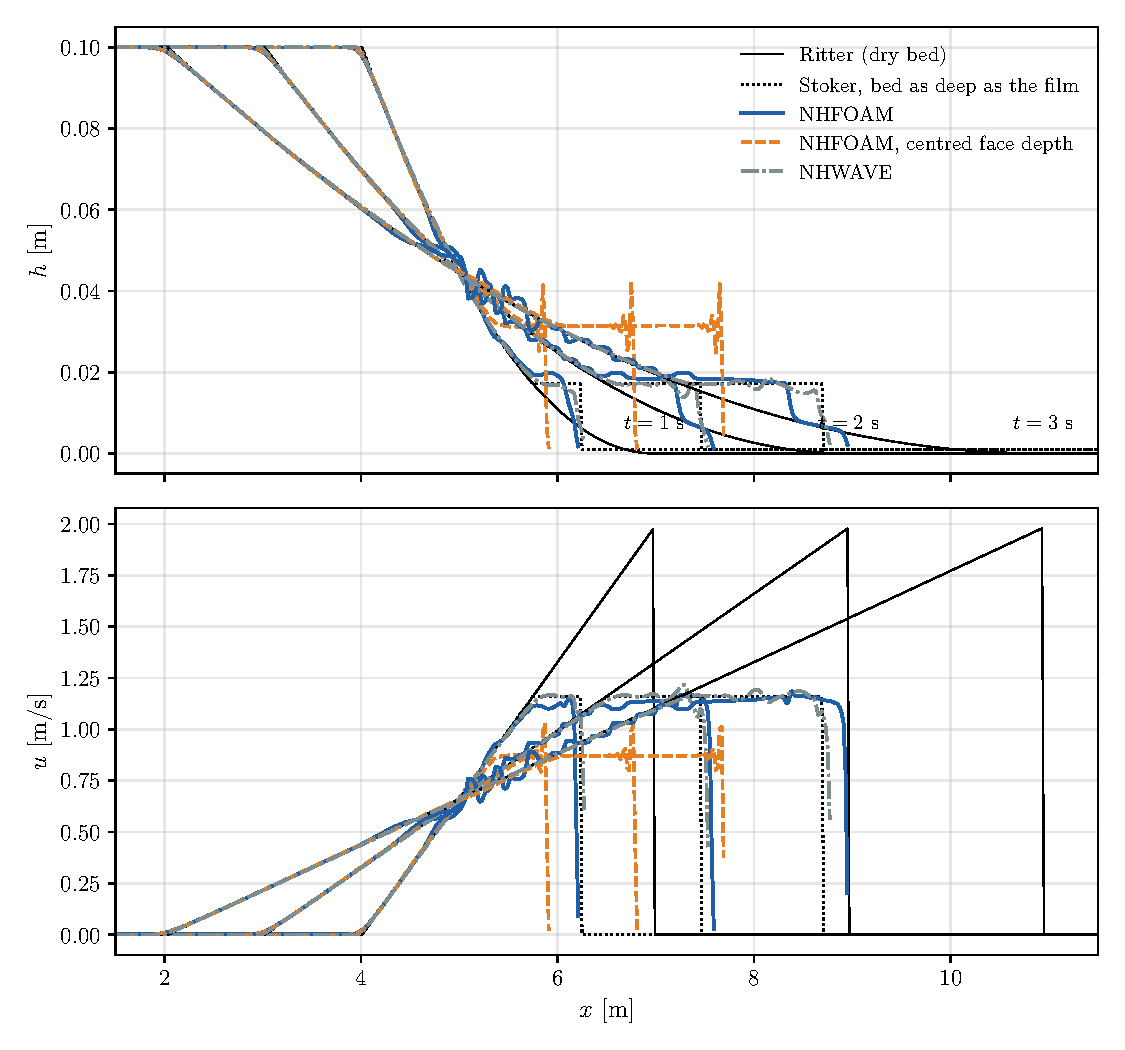
\includegraphics[width=0.85\textwidth]{wd_dambreak.pdf}
\caption{Dam break on a dry bed: depth and velocity at $t = 1$, 2 and 3 s.}
\label{fig:wd-dambreak}
\end{figure}

\subsection{Breaking solitary wave on a beach (test 4.5 of Ma et al.)}
\label{sec:wd-runup}

A solitary wave of $H/d = 0.28$ in $d = 0.21$ m breaks on a 1:20 beach
\citep{synolakis1987}, benchmark 4 of the NTHMP \citep{synolakis2008}, whose
data give the measured profiles. The set-up is NHWAVE's example
\code{solitary\_wave\_breaking}: toe at $x = 4$ m, the still-water shoreline at
8.2 m, dry beach up to 11 m, $\Delta x = 2$ cm, 3 layers, a 5 mm film. Both
models start from the solitary wave with its crest $d\,\mathrm{acosh}(\sqrt{20})/\gamma$
offshore of the toe ($\gamma = \sqrt{3H/4d}$), from the exact solution of
\citet{babenko1987} rather than NHWAVE's boundary wavemaker. NHWAVE's example
runs without bottom friction (no viscous terms, free-slip bottom), and so does
\NHFOAM\ here. \NHFOAM\ uses the hydrostatic front approximation and
\code{limitedLinearV}, with $\Delta t = 2$ ms.

The profiles (Fig.~\ref{fig:wd-runup}) agree with the measurements and with
NHWAVE during shoaling ($t^* = t\sqrt{g/d} = 10$, 15). At breaking ($t^*=20$)
\NHFOAM's bore is 0.04$d$ higher than NHWAVE's and the measured one. The
uprush ($t^* = 25$, 30) and the backwash with its hydraulic jump at
$x \approx 2.3d$ ($t^* = 50$) follow NHWAVE closely. The maximum run-up
(Fig.~\ref{fig:wd-shoreline}) is $R/d = 0.531$ at $t^* = 42.5$, against 0.512
at $t^* = 44$ for NHWAVE and 0.487--0.551 in the experiments with
$H/d = 0.26$--0.30. With the first-order upwind depth it is the same, 0.531;
with the centred depth 0.41; with $C_d = 0.006$ it is 0.464. In the backwash
the highest wet column of \NHFOAM\ recedes more slowly than NHWAVE's, because
thin puddles of up to a few millimetres above the film remain on the upper
beach. NHWAVE spreads such remnants with the depth diffusion of its HLL flux,
and its clip to the film does not conserve volume.

\begin{figure}[ht]
\centering
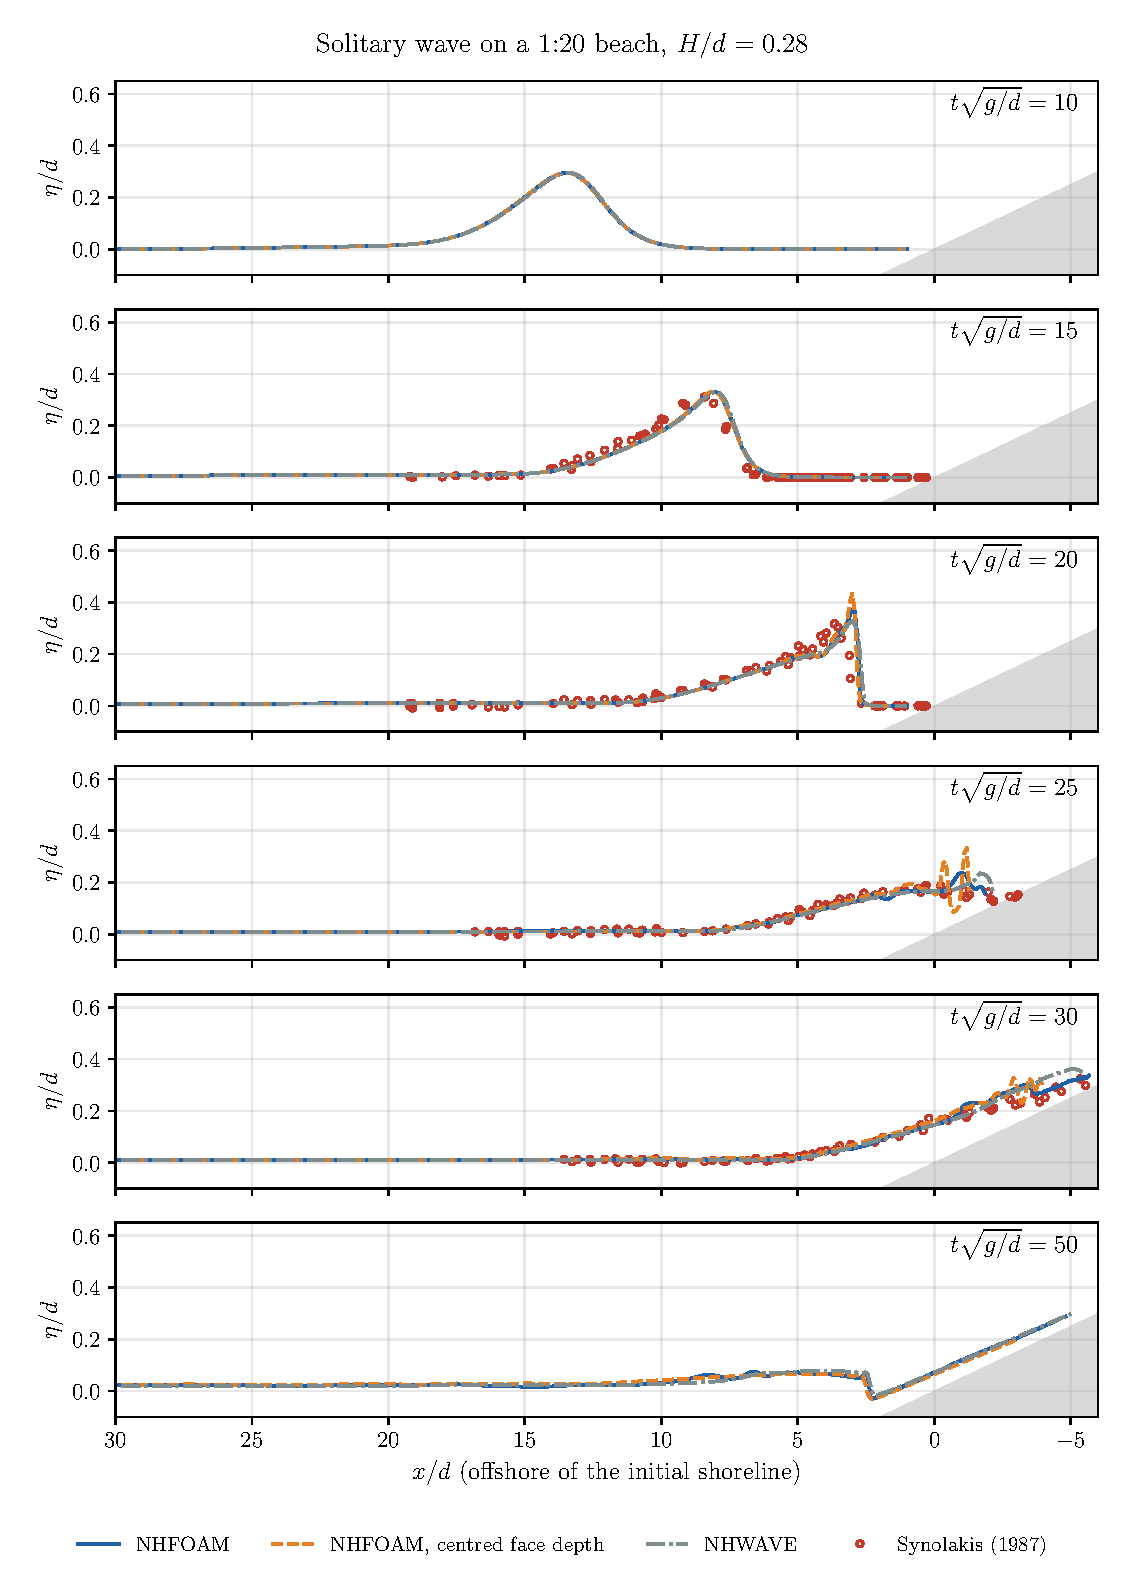
\includegraphics[width=0.88\textwidth]{wd_runup.pdf}
\caption{Solitary wave on a 1:20 beach, $H/d = 0.28$: surface profiles against
the measurements \citep{synolakis1987}.}
\label{fig:wd-runup}
\end{figure}

\begin{figure}[ht]
\centering
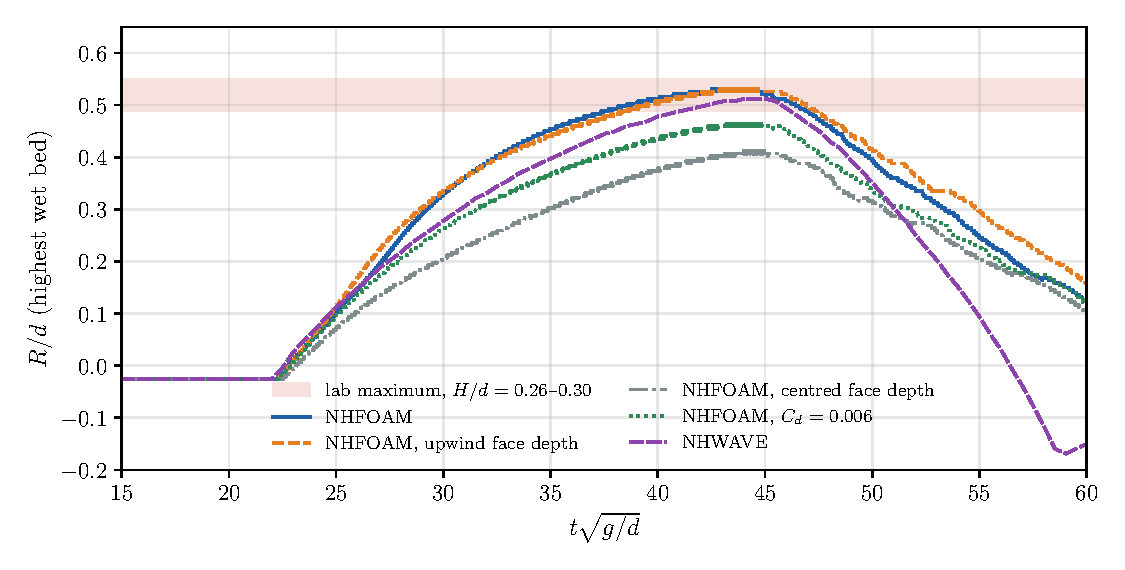
\includegraphics[width=0.9\textwidth]{wd_runup_shoreline.pdf}
\caption{Solitary wave on a 1:20 beach: highest wet bed over time. The band
is the range of the measured maximum run-up for $H/d = 0.26$--0.30.}
\label{fig:wd-shoreline}
\end{figure}

The first versions of the method failed this test in instructive ways. With
the centred depth and newly flooded columns starting from rest, the run-up was
$R/d = 0.37$--0.41, and the swash had grid-scale oscillations of the depth:
columns of 5 mm between columns of 5 cm, flooding and drying every step.
Giving a flooded column the velocity of the neighbour that flooded it
overshot to $R/d = 0.66$: a film with that velocity floods the next column in
the next step, and it ran away to the end of the beach. The upwind face
depth, the supercritical flux and the rules for opened faces and puddles
removed both problems.

\subsection{Solitary waves on a conical island}
\label{sec:wd-island}

\citet{briggs1995} sent solitary waves of $H/d = 0.045$, 0.091 and 0.181
(cases A, B, C; $d = 0.32$ m) against a conical island with a toe radius of
3.6 m, a crest radius of 1.1 m and 1:4 faces, and recorded the water level in
front of the island (gauges 1--4), on its front face (6, 9), on its side (16)
and behind it (22), and the run-up all round \citep[see also][]{liu1995}. It
is benchmark 6 of the NTHMP \citep{synolakis2008}, one of NHWAVE's examples
(\code{Solitary\_wave\_on\_a\_conical\_island}) and the first test of wetting
and drying in three dimensions here.

Both models use the settings of NHWAVE's example: 3 layers, $C_d = 0.01$, a
5 mm film, NHWAVE with its $k$--$\varepsilon$ model and \NHFOAM\ with the
hybrid breaking model of Section~\ref{sec:brk}. To keep the cost down they
cover half the basin, cut along the line through the centre of the island (a
slip wall, so that gauges 1 and 2 are the mirror images of 4 and 3), and start
from the exact solitary wave with $\eta = H/20$ at the incident gauges, as in
Section~\ref{sec:wd-runup}, instead of NHWAVE's boundary wavemaker. The basin
ends in a 2 m sponge. Each run is shifted in time so that its crest meets the
measured one at the incident gauges, and each measured record starts from its
mean before the wave. The run-up is the highest water level of the cells on
the edge of the flooded area, in sectors of $5^\circ$: \NHFOAM\ records it in
the new field \code{etaMax}, NHWAVE in \code{hmax}, and NHWAVE's own script
for this benchmark uses the same cells. NHWAVE's runs are on the 10 cm grid
only. On its own 5 cm grid one case would take about 5 h here, because its
time step follows the vertical Courant number of its thinnest layers and falls
to about 0.01 s in the thin water on the island.

On the same grid the two models agree closely (Figs.~\ref{fig:wd-island} and
\ref{fig:wd-island-runup}, Table~\ref{tab:wd-island}): the crests at the
incident gauges and at gauges 6, 9 and 16 within 4\% of each other, the run-up
within $0.01d$ in case A and within $0.02d$ on average in cases B and C. They
differ most behind the island, where the two fronts that wrapped round it
collide. At gauge 22 NHWAVE's crest is 5\% and 11\% higher than \NHFOAM's in
cases A and B, and 13\% lower in case C, where the waves break and NHWAVE's
crest is the closer to the measured one; \NHFOAM's also comes 0.3 s late. On
the flanks of the run-up peak behind the island ($75^\circ$--$105^\circ$) the
run-up differs by up to $0.08d$. Without its breaking model \NHFOAM\ gives the
same crest at gauge 22 (10.4 cm against 10.3 cm) and the same run-up, so its
breaking model hardly acts in the collision.

Against the measurements both models overshoot on the island's face (gauge 9,
11--22\%) and behind it in the smaller waves (gauge 22, 7--25\% in cases A and
B), as do the FUNWAVE results that come with NHWAVE's example (gauge 9: 17--25\%,
gauge 22: 47\% in case A and 31\% in B). The run-up has the measured shape:
highest in front, lowest at the sides, with a peak behind the island where the
fronts meet. In cases A and C the measured minima at $45^\circ$--$135^\circ$
are deeper than either model gives; in case B the models follow them but stay
below the measured peak behind the island ($0.28d$ against 0.19--$0.22d$). In
case C both stay below the measured front run-up of $0.55d$: 0.42--$0.45d$ on
the 10 cm grid and $0.47d$ for \NHFOAM\ on the 5 cm grid. After the crests the
measured troughs are deeper than both models give (case A: $-0.9$ cm against
$-0.4$ cm at the incident gauges, $-1.1$ cm against $-0.6$ to $-0.7$ cm at
gauge 6). The measured records also sit about 1 mm below the still-water level
after the incident crest, so part of this probably comes from the paddle's
wave, which was not an exact solitary wave.

Refining \NHFOAM's grid from 10 to 5 cm brings the run-up closer to the
measurements in cases B and C (rms error 0.039 to $0.024d$ and 0.070 to
$0.052d$) and changes the gauges by a few per cent, except gauge 22, whose
crests rise further above the measured ones (case A: from 13 to 25\%, case C:
from 13 to 28\%). On the same grid \NHFOAM\ ran 3 to 6 times faster than
NHWAVE.

\begin{table}[htbp]
\centering
\caption{Conical island: error of the highest crest at the gauges, run-up
$R/d$ in front of ($270^\circ$) and behind ($90^\circ$) the island, rms error
of the run-up over the measured points, and run time on 2 cores.}
\label{tab:wd-island}
\footnotesize
\setlength{\tabcolsep}{4pt}
\begin{tabular}{llrrrrrrrr}
\toprule
case & run & g6 & g9 & g16 & g22 & $R/d$ front & $R/d$ back & rms $R/d$ & time \\
\midrule
A & lab & & & & & 0.100 & 0.070 & & \\
  & \NHFOAM, 5 cm & +15\% & +19\% & +1\% & +25\% & 0.112 & 0.081 & 0.018 & 76 min \\
  & \NHFOAM, 10 cm & +15\% & +21\% & +3\% & +13\% & 0.104 & 0.087 & 0.014 & 7 min \\
  & NHWAVE, 10 cm & +12\% & +20\% & +3\% & +18\% & 0.107 & 0.089 & 0.016 & 22 min \\
\midrule
B & lab & & & & & 0.230 & 0.269 & & \\
  & \NHFOAM, 5 cm & +8\% & +14\% & +7\% & +15\% & 0.238 & 0.215 & 0.024 & 58 min \\
  & \NHFOAM, 10 cm & +8\% & +16\% & +9\% & +7\% & 0.220 & 0.188 & 0.039 & 5 min \\
  & NHWAVE, 10 cm & +6\% & +11\% & +8\% & +19\% & 0.229 & 0.205 & 0.032 & 21 min \\
\midrule
C & lab & & & & & 0.547 & 0.341 & & \\
  & \NHFOAM, 5 cm & +4\% & +22\% & +8\% & +28\% & 0.473 & 0.301 & 0.052 & 42 min \\
  & \NHFOAM, 10 cm & +3\% & +18\% & +12\% & +13\% & 0.422 & 0.285 & 0.070 & 4 min \\
  & NHWAVE, 10 cm & +1\% & +14\% & +12\% & $-2$\% & 0.454 & 0.291 & 0.067 & 27 min \\
\bottomrule
\end{tabular}
\end{table}

\begin{figure}[htbp]
\centering
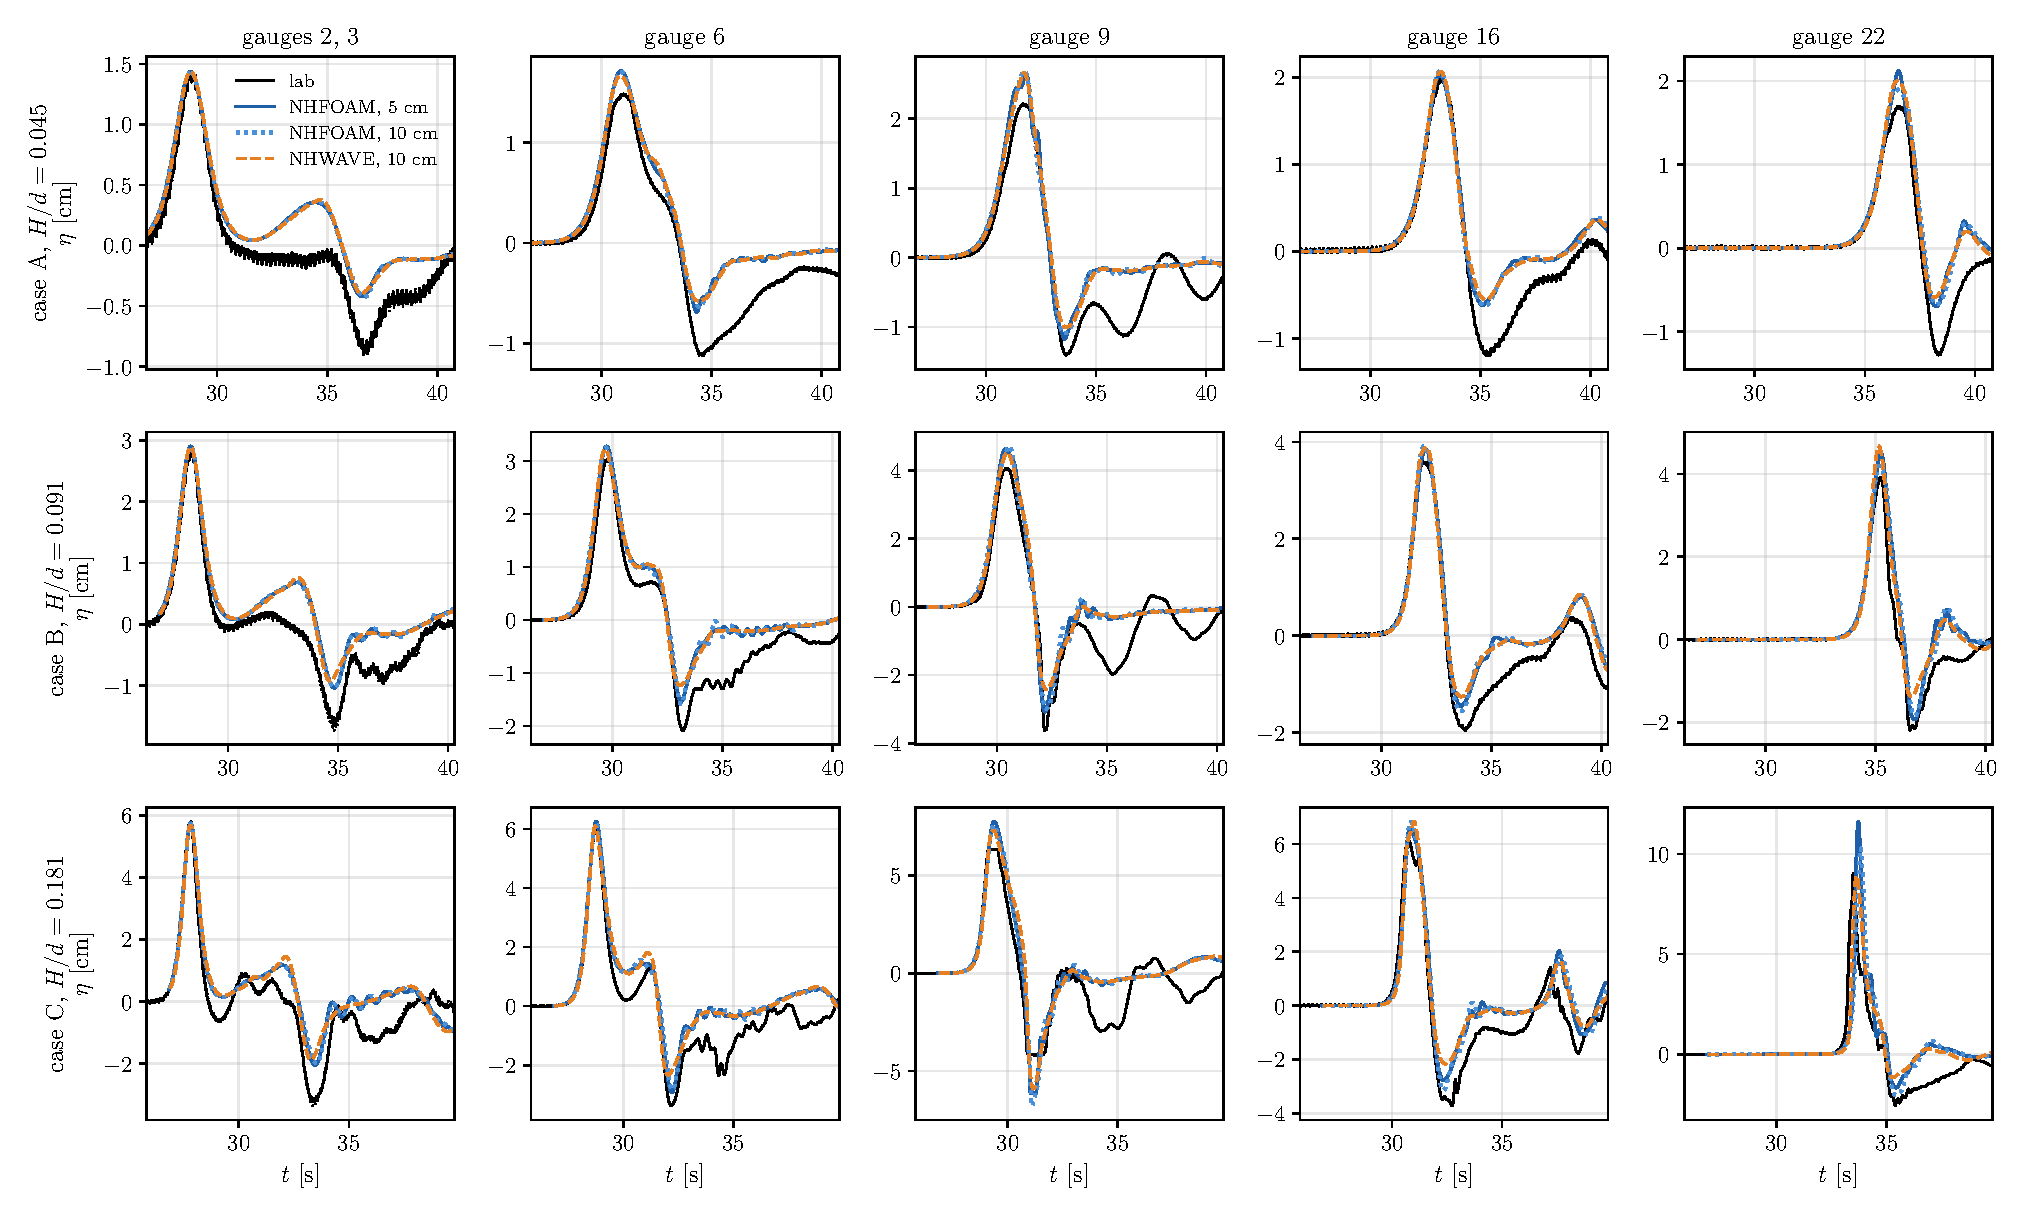
\includegraphics[width=\textwidth]{conical_island_gauges.pdf}
\caption{Solitary waves on a conical island: water level at the gauges against
the measurements of \citet{briggs1995}. The first column shows lab gauges 2
(solid) and 3 (dotted); the model gauge sits at gauge 3, the mirror image of
gauge 2.}
\label{fig:wd-island}
\end{figure}

\begin{figure}[htbp]
\centering
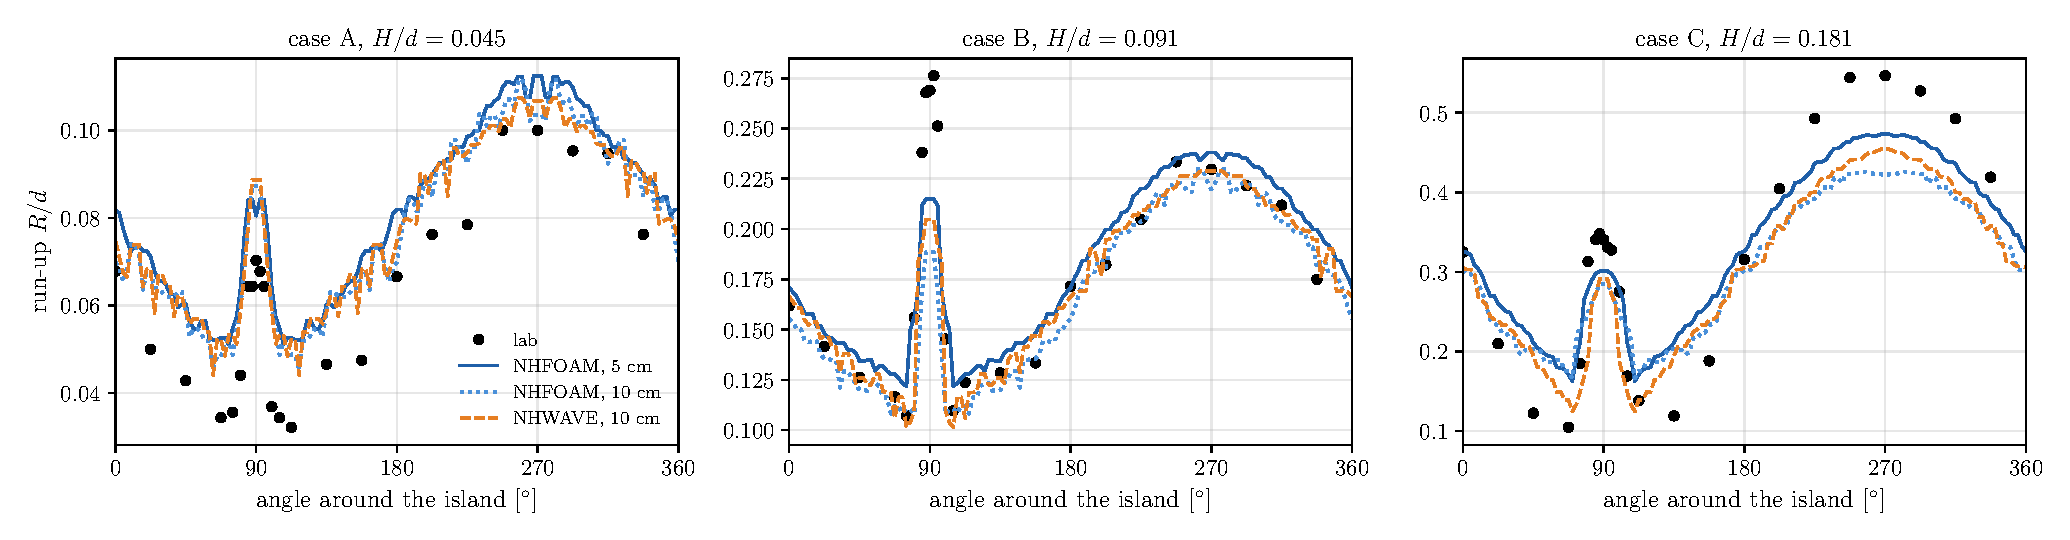
\includegraphics[width=\textwidth]{conical_island_runup.pdf}
\caption{Solitary waves on a conical island: run-up around the island
($0^\circ$ at gauge 16, $90^\circ$ behind the island, $270^\circ$ in front).}
\label{fig:wd-island-runup}
\end{figure}

\subsection{Tsunami run-up in the Monai valley}
\label{sec:wd-monai}

The 1993 Hokkaido Nansei-Oki tsunami ran up 31.7 m at the head of a narrow
valley near Monai, on Okushiri Island. \citet{matsuyama2001} rebuilt the
coast at 1:400 in a 205 m long, 3.5 m wide tank of the Central Research
Institute for Electric Power Industry. The experiment was benchmark 2 of the
2004 workshop on long-wave run-up models \citep{liu2008}; it is benchmark 7
of the NTHMP \citep{synolakis2008} and one of NHWAVE's examples
(\code{Runup\_onto\_a\_complex\_3-D\_beach\_Monai\_Valley}). The benchmark
covers $5.488 \times 3.402$ m with the bed on a 1.4 cm grid: 13.5 cm of water
at $x = 0$, a small island in front of the valley, land up to 12.5 cm above
the still water, and walls on the other three sides. The incident wave is
given at $x = 0$ for 22.5 s, a depression of 2.9 mm followed by a crest of
16.1 mm ($H/d = 0.12$). Gauges 5, 7 and 9 recorded the water level at
$x = 4.521$ m, where the bed file has only 1.2, 0.3 and 0.6 cm of water. In
six repeats the wave ran up 8.0--10.0 cm (mean 9.0 cm) at the head of the
valley, which narrows to 4--6 cm there, and 5.25--6.75 and 5.25--5.75 cm at
two points on its north side.

\NHFOAM\ covers the benchmark domain and takes the incident wave at $x = 0$
as a time series (Section~\ref{sec:ts}) with the active absorption, so that
the boundary lets the reflected waves out, also after 22.5 s, when the
record (tapered to zero over its last 0.5 s) ends. The velocity is uniform
over the depth, $u = c\eta/(d+\eta)$ with $c = \sqrt{g(d+\eta)}$. NHWAVE runs
its example: the domain extended 1.4 m offshore, its internal wavemaker
between $x = -0.14$ and 0 m driven by a Fourier fit of the record (399
components), a 1 m sponge behind it and its $k$--$\varepsilon$ model. Both
models use 4 layers, log-law friction with a roughness of 0.1 mm (NHWAVE's
\code{Zob}) and NHWAVE's 2 mm film; \NHFOAM\ runs its hybrid breaking model.
\NHFOAM\ runs on the benchmark grid (1.4 cm, $392\times243$ columns) and on
the grid coarsened twice (2.8 by 2.79 cm, $196\times122$ columns). On the
benchmark grid NHWAVE takes about 10 s per time step on two cores, about
16 h for the 25 s, so it runs on the coarse grid, with the bed interpolated from the
benchmark nodes and the cell depths the means of the four corners, as
NHWAVE's own depth file has them on the fine grid. On the coarse grid each
model also runs without its breaking treatment (\NHFOAM\ without the
breaking model, NHWAVE without $k$--$\varepsilon$). No run is shifted in
time, and the measured records are shown as given (they read $+2$ to $+5$
mm before the wave arrives). The run-up is the highest ground that a model
floods (the highest bed among the columns that were ever wet), which is how
it was measured: the ground at the three lab points is 8.9, 6.2 and 5.5 cm
high, their mean run-ups. The shorelines at the times of the video frames
of the experiment come from the new \NHFOAM\ option
\code{surfaceSnapshots}, which writes the free surface of every column at
listed times without the full fields, and from NHWAVE's surface output every
0.1 s; the photographs themselves were not compared.

On both grids \NHFOAM's first column follows the record to 0.2 mm rms over
the first 12 s, before the waves reflected from the island and the coast
come back (Fig.~\ref{fig:wd-monai}a). NHWAVE's wavemaker keeps time with the
record too (lag 0.001 s), with a deeper depression (3.5 against 2.9 mm) and
a 2\% lower crest (0.6 mm rms). After 12 s both boundaries let the same
reflected waves out.

The depression dries all three gauge columns in both models (the flat parts
of Fig.~\ref{fig:wd-monai} at 12--15 s), while the measured records stay wet:
gauge 7 reads 0.6 cm below the still water at 14 s, where the bed file puts
the bed at $-0.27$ cm, so the gauges stood in deeper water than the file has
at their positions. The bore then floods the dried bed. \NHFOAM's arrives
0.03--0.39 s after the measured one on both grids, NHWAVE's 0.30--0.40 s,
about the 0.4 s by which NHWAVE's example shifts its results
(Table~\ref{tab:wd-monai}). Behind the bore both models follow the measured
records, with rms differences of 0.5--0.6 cm. \NHFOAM's short crests at
17--17.6 s are 13--18\% higher than the measured ones on the coarse grid and
21--29\% on the benchmark grid; NHWAVE's smoother crests are 1--5\% lower.

On the coarse grid the two models flood almost the same columns (0.64 and
0.63 m$^2$ of land; \NHFOAM\ floods every column that NHWAVE floods) and run
up 6.6 cm at the head of the valley, 27\% below the measured mean, and
4.3 cm at the two points to the north, 23--29\% low
(Fig.~\ref{fig:wd-monai-runup}, Table~\ref{tab:wd-monai-runup}): the head of
the valley is only one or two coarse cells wide. On the benchmark grid
\NHFOAM\ runs up 7.4 cm at the head (17\% low, below the lowest of the six
repeats), 5.4 cm at the first point to the north (within the measured
5.25--6.75 cm) and 4.4 cm at the second (21\% low). The shorelines of the two
grids agree at the times of the video frames (Fig.~\ref{fig:wd-monai-frames});
NHWAVE's lags behind \NHFOAM's while the water climbs the valley (by 0.27 m
at 15.3 s and 0.17 m at 15.8 s) and has caught up by 16.8 s.

Without its breaking model \NHFOAM's crest at gauge 5 is 9\% higher (4.70
against 4.31 cm), and the bore, the rms differences and the run-up do not
change. Without $k$--$\varepsilon$ NHWAVE's crests are 1--3\% higher and its
bore arrives 0.02 s earlier, with the same run-up. Neither closure explains
the differences between the models: with or without them NHWAVE's bore
reaches gauges 7 and 9 0.3 s after \NHFOAM's, and \NHFOAM's short crests
stay 11--29\% above NHWAVE's. The difference lies in how the bore runs over
the dried bed: NHWAVE's shoreline also lags behind \NHFOAM's while the water
climbs the valley.
On the coarse grid \NHFOAM\ took 35 min and NHWAVE 2.0 h on two cores
(1.7 h without $k$--$\varepsilon$); \NHFOAM\ took 6.2 h on the benchmark
grid.

\begin{table}[htbp]
\centering
\caption{Monai valley, gauges over 13--23 s: highest crest against the
measured one, arrival of the bore ($\eta$ rising through 0.5 cm) against the
measured arrival, and rms difference.}
\label{tab:wd-monai}
\footnotesize
\setlength{\tabcolsep}{4pt}
\begin{tabular}{lrrrrrrrrr}
\toprule
run & \multicolumn{3}{c}{crest} & \multicolumn{3}{c}{bore arrival [s]} & \multicolumn{3}{c}{rms [cm]} \\
\cmidrule(lr){2-4}\cmidrule(lr){5-7}\cmidrule(lr){8-10}
 & g5 & g7 & g9 & g5 & g7 & g9 & g5 & g7 & g9 \\
\midrule
lab & 3.70 cm & 3.92 cm & 4.54 cm & 14.59 & 14.81 & 14.95 & & & \\
\NHFOAM, 1.4 cm & +21\% & +24\% & +29\% & +0.39 & +0.11 & +0.03 & 0.58 & 0.52 & 0.58 \\
\NHFOAM, 2.8 cm & +16\% & +13\% & +18\% & +0.36 & +0.12 & +0.03 & 0.57 & 0.53 & 0.59 \\
NHWAVE, 2.8 cm & $-3$\% & $-1$\% & $-5$\% & +0.34 & +0.40 & +0.30 & 0.62 & 0.53 & 0.58 \\
\NHFOAM, 2.8 cm, no breaking & +27\% & +14\% & +20\% & +0.36 & +0.11 & +0.03 & 0.58 & 0.53 & 0.60 \\
NHWAVE, 2.8 cm, no $k$--$\varepsilon$ & $-1$\% & +2\% & $-3$\% & +0.32 & +0.38 & +0.28 & 0.62 & 0.52 & 0.60 \\
\bottomrule
\end{tabular}
\end{table}

\begin{table}[htbp]
\centering
\caption{Monai valley: run-up at the measured points, the head of the
valley (5.158, 1.880) m and two points on its north side, N1 (5.030, 2.206)
m and N2 (4.998, 2.320) m (lab: the six repeats), the
highest flooded ground in the valley ($1.75 < y < 2.05$ m), the flooded land
and the run time on two cores.}
\label{tab:wd-monai-runup}
\footnotesize
\setlength{\tabcolsep}{4pt}
\begin{tabular}{lrrrrrr}
\toprule
run & \multicolumn{3}{c}{run-up at the lab points [cm]} & highest in the & flooded & time \\
\cmidrule(lr){2-4}
 & head & N1 & N2 & valley [cm] & land [m$^2$] & \\
\midrule
lab, range & 8.0--10.0 & 5.25--6.75 & 5.25--5.75 & & & \\
lab, mean & 9.0 & 6.0 & 5.6 & & & \\
\NHFOAM, 1.4 cm & 7.4 & 5.4 & 4.4 & 7.5 & 0.65 & 6.2 h \\
\NHFOAM, 2.8 cm & 6.6 & 4.3 & 4.3 & 6.9 & 0.64 & 35 min \\
NHWAVE, 2.8 cm & 6.6 & 4.3 & 4.3 & 6.6 & 0.63 & 2.0 h \\
\NHFOAM, 2.8 cm, no breaking & 6.6 & 4.3 & 4.3 & 6.9 & 0.64 & 35 min \\
NHWAVE, 2.8 cm, no $k$--$\varepsilon$ & 6.6 & 4.3 & 4.3 & 6.6 & 0.64 & 1.7 h \\
\bottomrule
\end{tabular}
\end{table}

\begin{figure}[htbp]
\centering
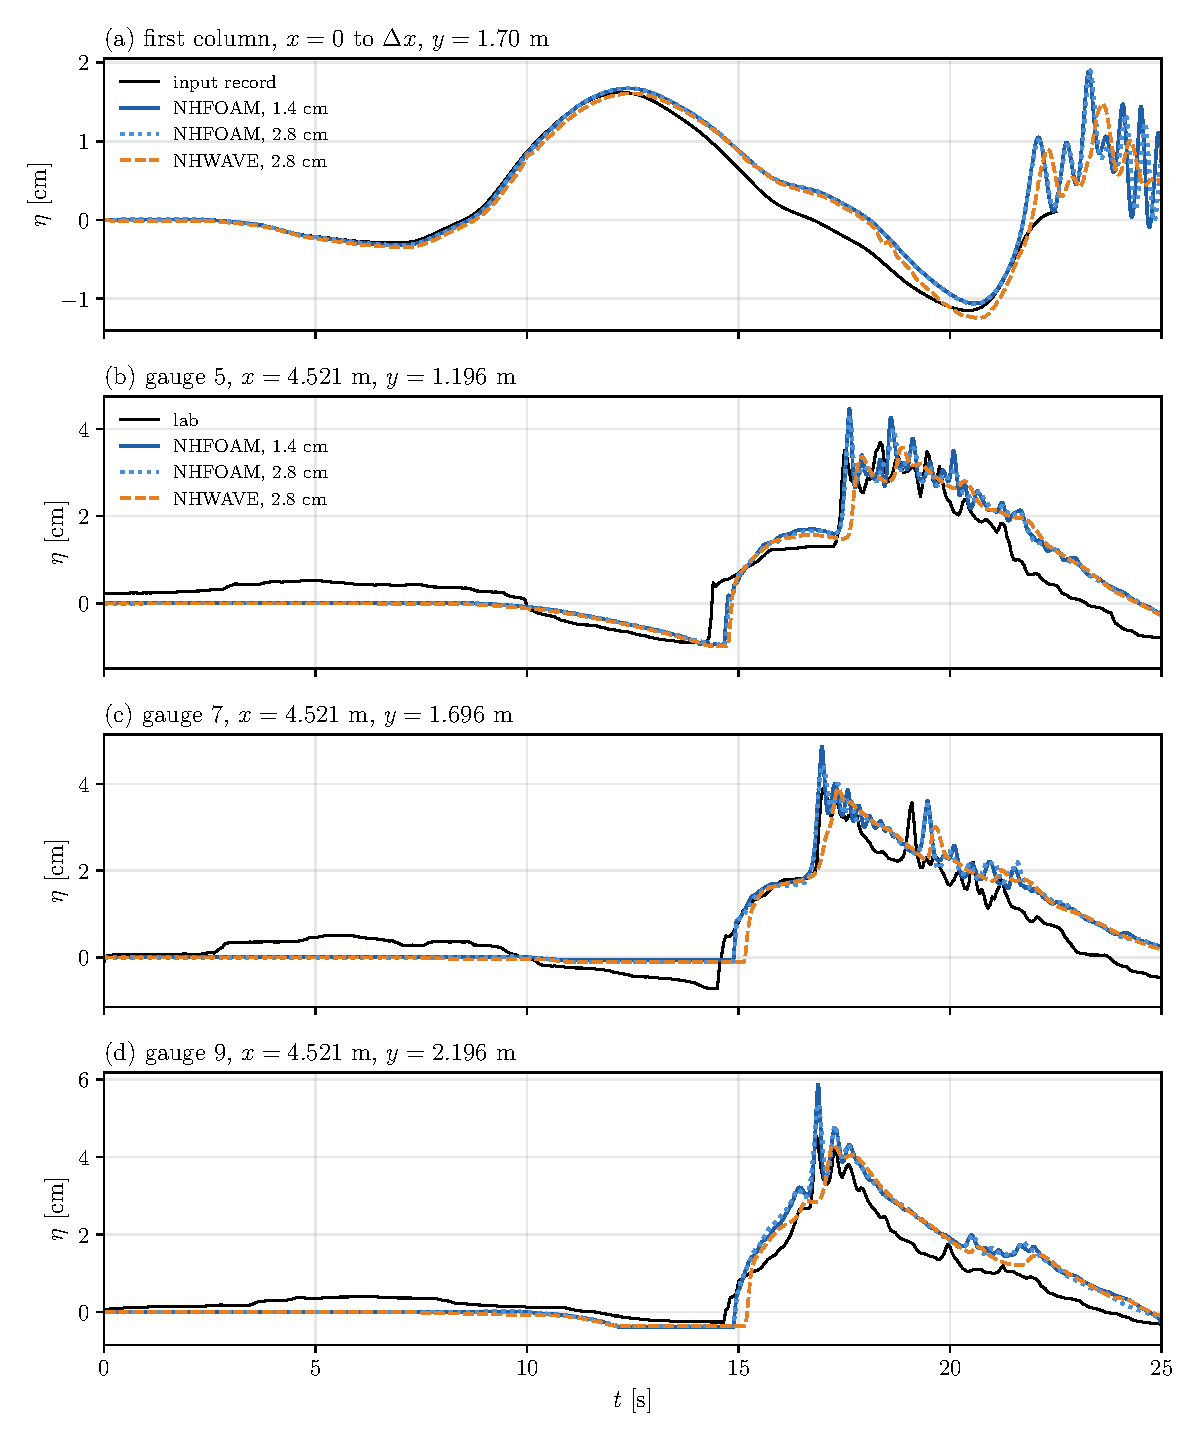
\includegraphics[width=0.85\textwidth]{monai_valley_gauges.pdf}
\caption{Monai valley: (a) the surface of the first column ($y = 1.70$ m)
against the input record; (b--d) water level at gauges 5, 7 and 9 against
the measurements of \citet{matsuyama2001}.}
\label{fig:wd-monai}
\end{figure}

\begin{figure}[htbp]
\centering
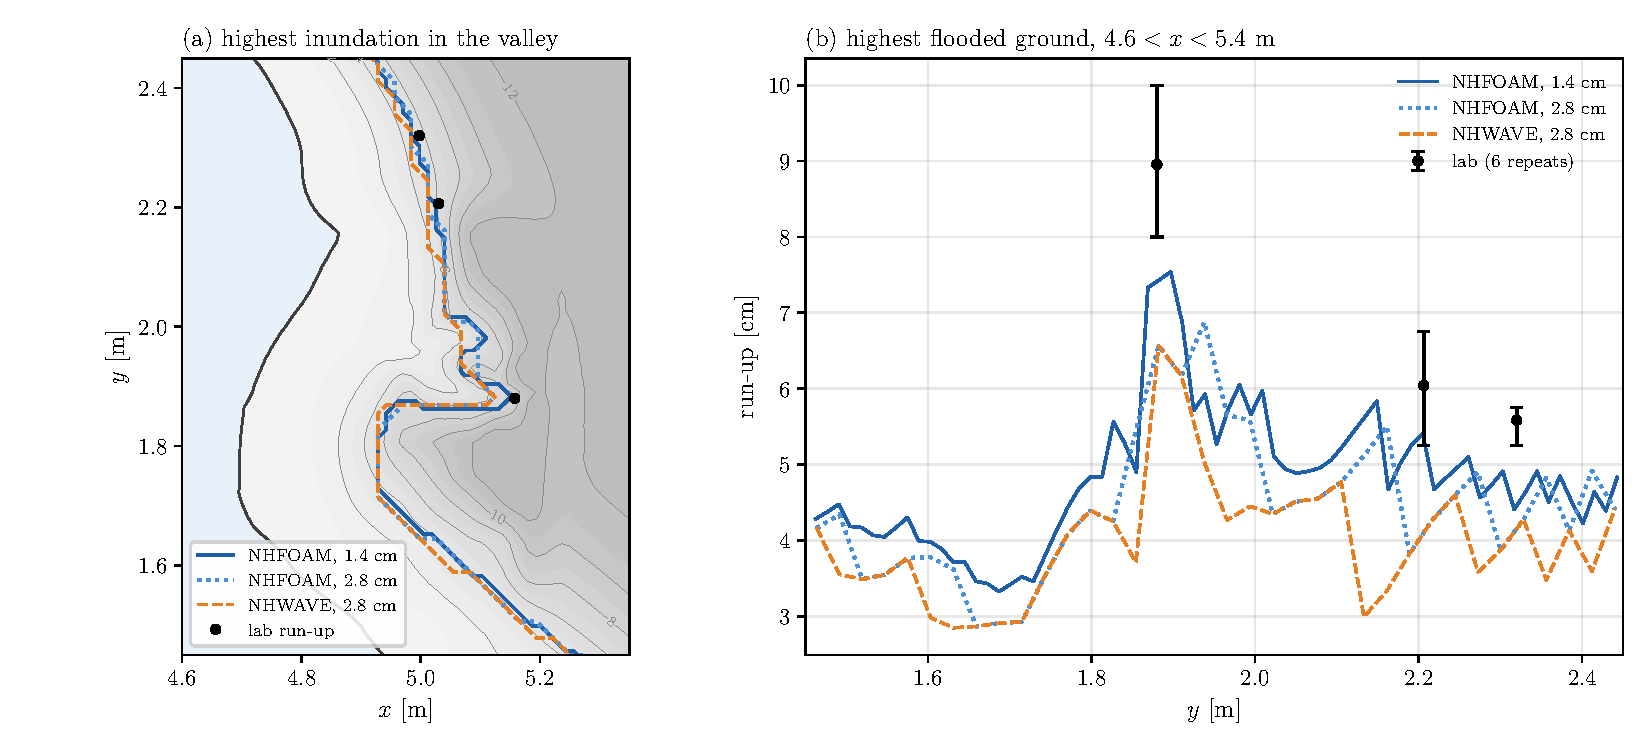
\includegraphics[width=\textwidth]{monai_valley_runup.pdf}
\caption{Monai valley: (a) the edge of the flooded area around the valley
(ground shaded by its height, contours every 2 cm, the still-water shoreline
thick) and the points of the measured run-up; (b) the highest flooded ground
along the valley ($4.6 < x < 5.4$ m) against the measured run-up (range of
the six repeats).}
\label{fig:wd-monai-runup}
\end{figure}

\begin{figure}[htbp]
\centering
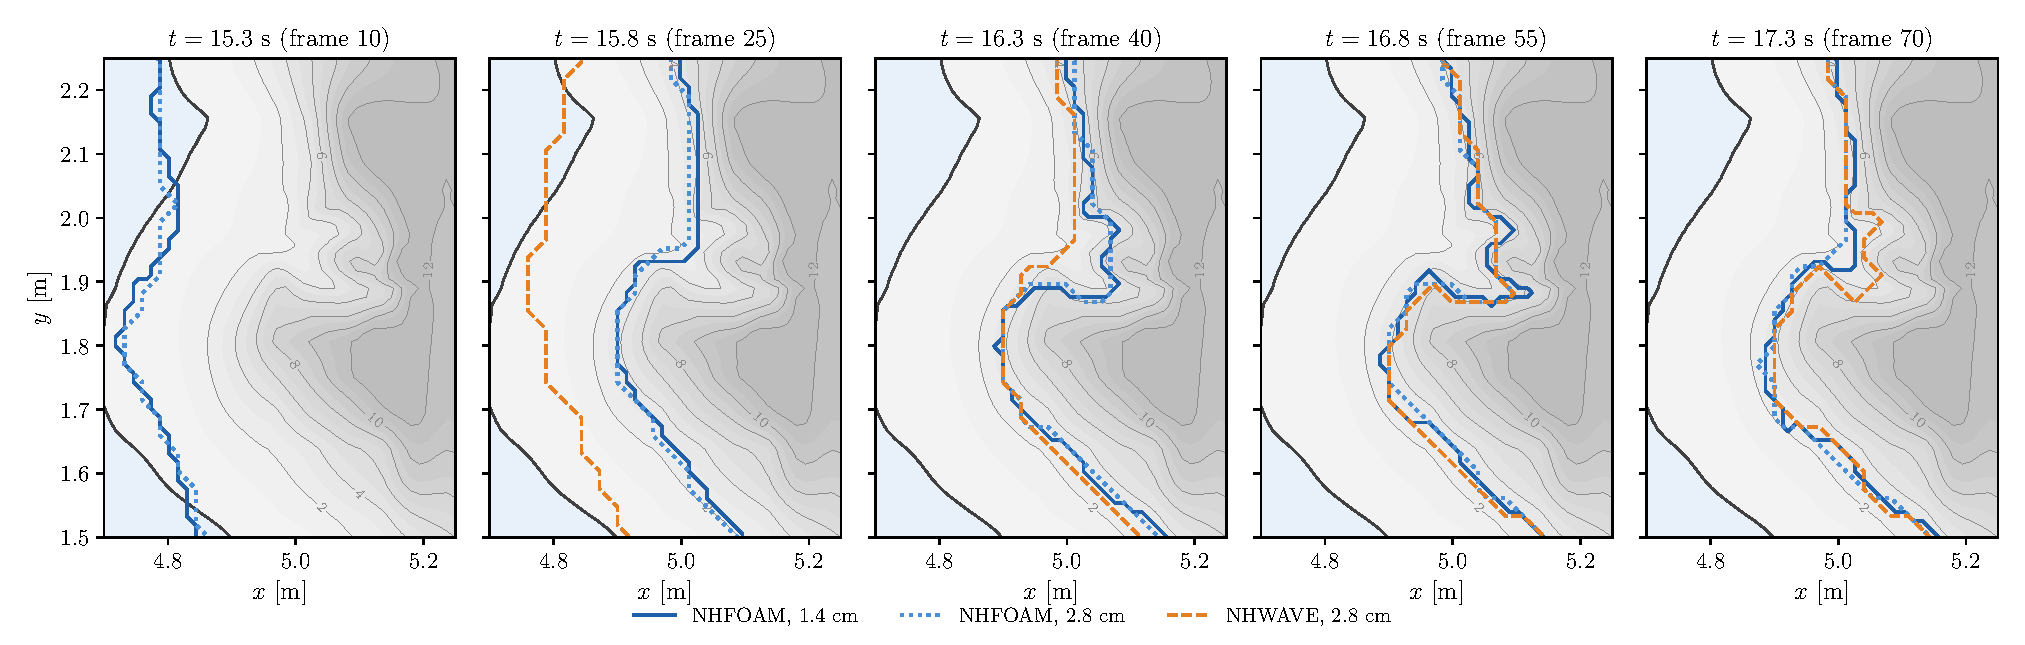
\includegraphics[width=\textwidth]{monai_valley_frames.pdf}
\caption{Monai valley: shorelines at the times of frames 10--70 of the video
of the experiment ($t = 15.3$--17.3 s, as the benchmark gives them). At
15.3 s NHWAVE's shoreline still lies seaward of the frame ($x < 4.7$ m).}
\label{fig:wd-monai-frames}
\end{figure}

\subsection{The Monai valley on a mesh refined around the valley}
\label{sec:wd-monai-ref}

On the uniform grids the run-up at the head of the valley stays 17\%
(1.4 cm) to 27\% (2.8 cm) below the measured mean. The valley narrows to
4--6 cm there, and a uniform grid pays for the resolution of the valley over
the whole basin. NHWAVE has no other choice; \NHFOAM\ takes any mesh that is
made of columns (Section~\ref{sec:unstr}). Here the basin is meshed with
gmsh quadrilaterals whose size follows the depth, $5.6\sqrt{h/d}$ cm down to
2.8 cm in the shallow water and on the land that the wave can reach, with
smaller cells in a box of $0.45 \times 0.7$ m around the valley and the three
lab points and, as an option, on the shelf in front of it ($1.3 \times 1.5$
m, with the gauges), extruded into 4 layers (Fig.~\ref{fig:wd-monai-ref}a).
Everything else is the set-up of Section~\ref{sec:wd-monai}. The time step
follows the Courant number (at most 1) below 8 ms, the step of the uniform
2.8 cm grid, so the small cells cost time steps only while water moves
through them: the smallest step is 2--4 ms and the runs take 3150--3530
steps. The bed is still the bilinear interpolation of the 1.4 cm benchmark
data, so cells below 1.4 cm add numerical resolution and no detail of the
bed.

\begin{table}[htbp]
\centering
\caption{Monai valley on uniform grids and on meshes refined around the
valley: run-up at the head of the valley and at the two points to its north
(N1, N2), the highest flooded ground in the valley and the run time on two
cores.}
\label{tab:wd-monai-ref}
\footnotesize
\setlength{\tabcolsep}{4pt}
\begin{tabular}{lrrrrrrr}
\toprule
mesh & columns & steps & \multicolumn{3}{c}{run-up [cm]} & valley & time \\
\cmidrule(lr){4-6}
 & & & head & N1 & N2 & [cm] & \\
\midrule
lab, range & & & 8.0--10.0 & 5.25--6.75 & 5.25--5.75 & & \\
lab, mean & & & 9.0 & 6.0 & 5.6 & & \\
uniform 2.8 cm & 23\,912 & 3125 & 6.6 & 4.3 & 4.3 & 6.9 & 35 min \\
uniform 1.4 cm & 95\,256 & 6250 & 7.4 & 5.4 & 4.4 & 7.5 & 6.2 h \\
valley 1.4 cm & 16\,883 & 3150 & 7.0 & 4.7 & 4.3 & 7.4 & 16 min \\
shelf and valley 1.4 cm & 22\,962 & 3163 & 7.1 & 5.8 & 4.7 & 7.8 & 22 min \\
valley 0.7 cm & 22\,455 & 3264 & 8.1 & 5.7 & 4.9 & 8.3 & 22 min \\
shelf 1.4 cm, valley 0.7 cm & 28\,279 & 3282 & 8.1 & 5.6 & 5.1 & 8.2 & 28 min \\
valley 0.7 cm, head 0.35 cm & 24\,897 & 3528 & 8.5 & 5.8 & 5.1 & 8.5 & 27 min \\
valley 0.7 cm, triangles & 52\,929 & 3891 & 8.3 & 5.6 & 5.3 & 8.3 & 64 min \\
\bottomrule
\end{tabular}
\end{table}

The resolution of the valley decides the run-up
(Table~\ref{tab:wd-monai-ref}, Fig.~\ref{fig:wd-monai-ref}). With 0.7 cm
cells in the valley the run-up at the head is 8.1 cm, inside the measured
8.0--10.0 cm, and 5.7 cm at N1 (measured 5.25--6.75 cm); N2 stays 12\% below
the measured mean. That mesh has fewer columns than the uniform 2.8 cm grid
and ran in 22 min, against 6.2 h for the uniform 1.4 cm grid, which gives
7.4 cm: a quarter of the columns and, with the adaptive step that the
uniform runs did not use, half the time steps. With 1.4 cm on the shelf and
in the valley the refined mesh gives the run-up of the uniform 1.4 cm grid
within 0.3 cm at the three points and its crests at the gauges ($+21$, $+17$
and $+25\%$ against $+21$, $+24$ and $+29\%$). Meshes of the same nominal
resolution differ by 0.1--0.3 cm at a point, as the run-up is read from the
bed height of single columns.

The shelf matters for the gauges and not for the head of the valley: with
0.7 cm in the valley, the shelf at 1.4 cm instead of 2.8 cm leaves the
run-up at the head at 8.1 cm, while on every refined mesh the bore reaches
the gauges within 0.04 s of the uniform grid with the same resolution on the
shelf, with the same rms differences (0.50--0.60 cm). The run-up at the head
is not yet converged: with 0.35 cm cells there ($0.32 \times 0.22$ m) it
rises again, to 8.5 cm, so that from 2.8 to 0.35 cm it goes 6.6, 7.0--7.4,
8.1 and 8.5 cm (lab mean 9.0 cm).
The same mesh in triangles (edges of the same length, so 2.4 times the
columns) runs up 8.3, 5.6 and 5.3 cm, within 0.4 cm of the
quadrilaterals' 8.1, 5.7 and 4.9 cm, with the same gauges, at three
times the cost; the 8\% lower run-up of the triangulated strip of
Section~\ref{sec:unstr} does not show here.
The film is not the limit: on the uniform 2.8 cm grid, films of 2, 1 and
0.5 mm give the same run-up at all three points and crests within 5\% of
each other; with the thinner films the bore reaches
gauge 5 0.15 s earlier and gauge 9 0.07--0.11 s later.

\begin{figure}[htbp]
\centering
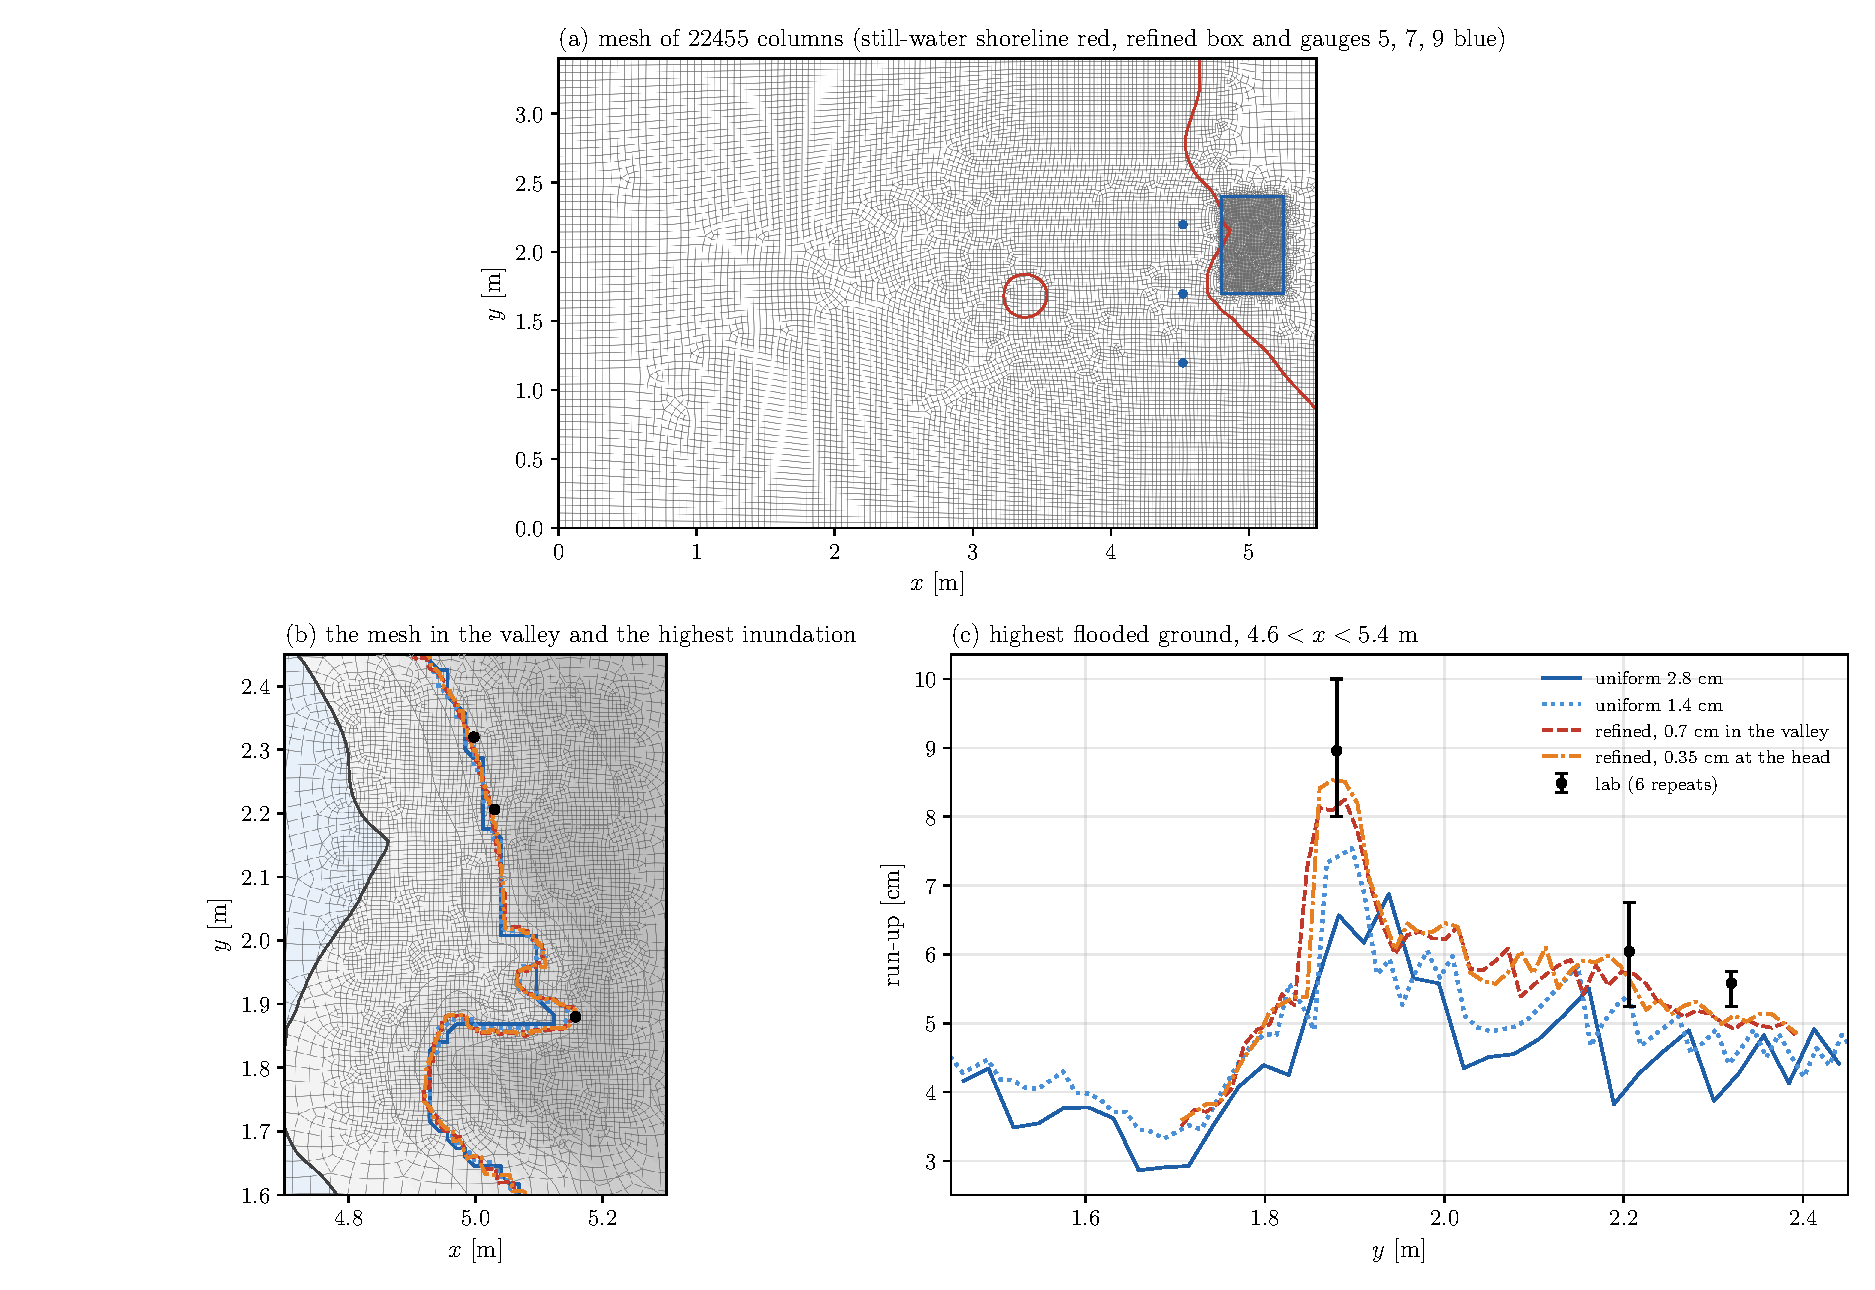
\includegraphics[width=\textwidth]{monai_valley_refined.pdf}
\caption{Monai valley on a mesh refined around the valley: (a) the mesh with
0.7 cm cells in the valley; (b) the mesh in the valley, the edge of the
flooded area and the points of the measured run-up; (c) the highest flooded
ground along the valley against the measured run-up (range of the six
repeats).}
\label{fig:wd-monai-ref}
\end{figure}

\subsection{Spilling breakers on a 1:35 beach}
\label{sec:wd-tk}

\citet{ting1994} measured spilling breakers of $H = 0.125$ m and $T = 2$ s from
$h = 0.4$ m on a 1:35 beach. Here $x$ is measured from the toe of the slope,
which reproduces the measured breaking point; the still-water shoreline is
at $x = 14$ m. \NHFOAM\ makes stream-function waves in a 3.8 m relaxation zone,
2.2 m ahead of the toe, and runs onto dry land up to $x = 17$ m: 10 layers,
$\Delta x = 2.5$ cm, $\Delta t = 5$ ms, a 5 mm film, $C_d = 0.006$, the
hydrostatic front approximation with $\alpha = 0.6$ and $\beta = 0.3$. NHWAVE
runs its example \code{tingkirby}, with 20 layers, the $k$--$\epsilon$ model, a
cnoidal wave at the boundary and a 2 cm film. Its bed has the toe 5.6 m from
the wavemaker, so its $x$ is shifted by 5.6 m. Both runs last 60 s, and the
statistics use the last 10 periods (Fig.~\ref{fig:wd-tk},
Table~\ref{tab:wd-tk}).

\begin{figure}[ht]
\centering
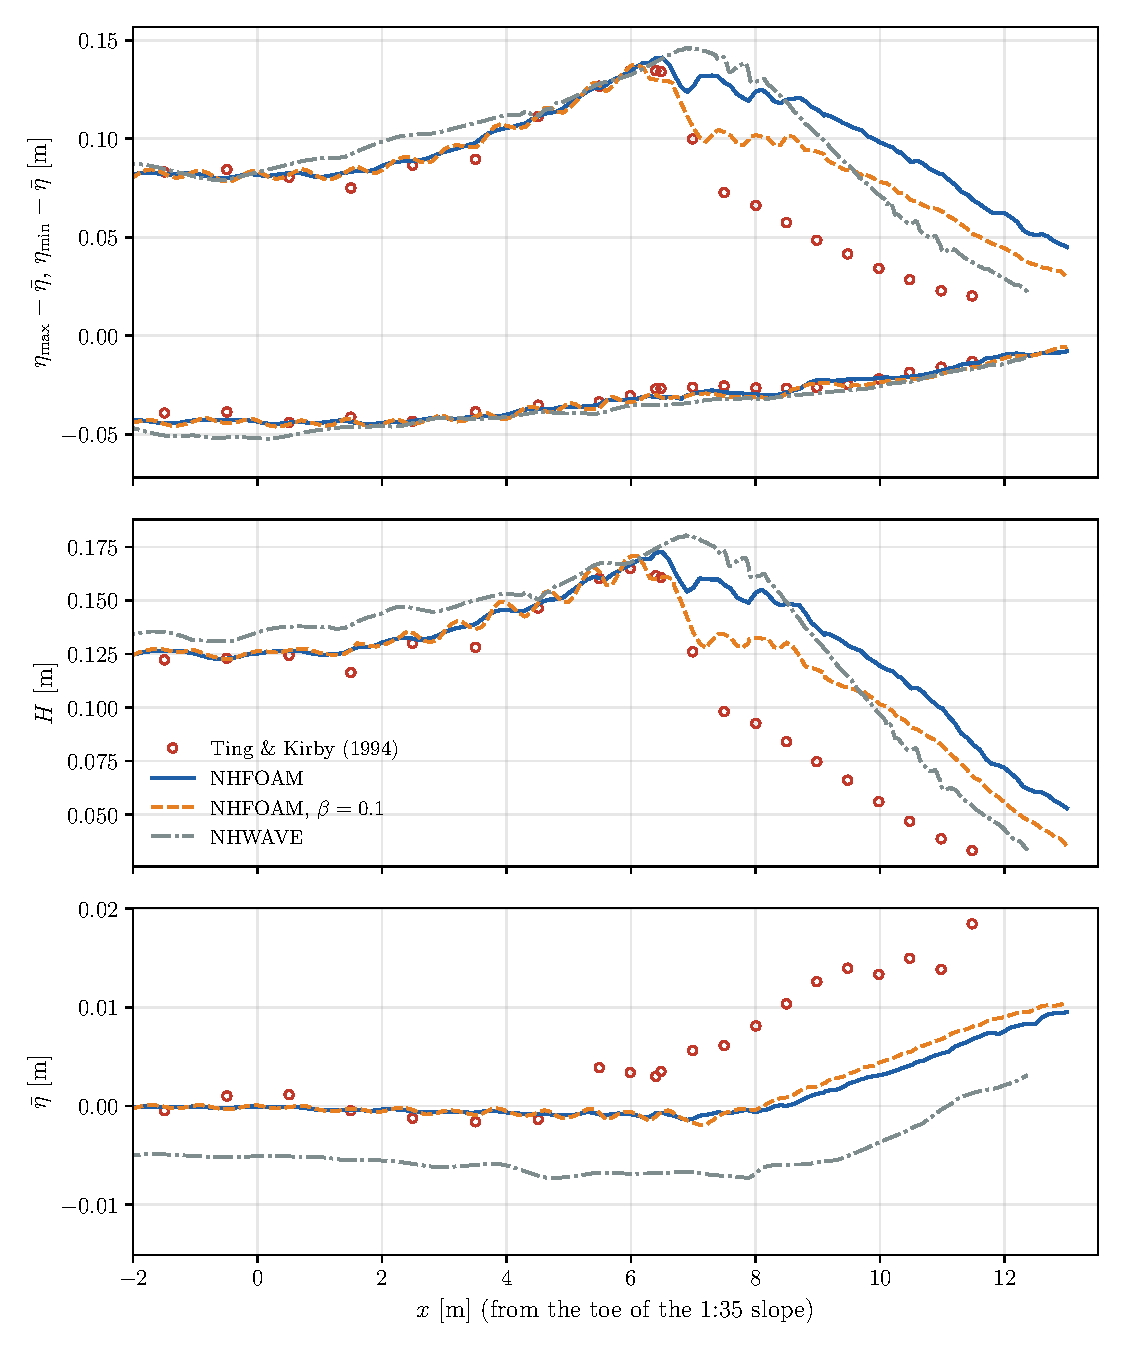
\includegraphics[width=0.9\textwidth]{tk_spilling.pdf}
\caption{Spilling breakers \citep{ting1994}: crest and trough relative to the
mean level, wave height and mean water level.}
\label{fig:wd-tk}
\end{figure}

\begin{table}[ht]
\centering
\caption{Spilling breakers: wave height and mean water level (cm).}
\label{tab:wd-tk}
\small
\begin{tabular}{lcccc}
\toprule
 & lab & \NHFOAM & \NHFOAM, $\beta = 0.1$ & NHWAVE \\
\midrule
$H$ at $x = -0.5$ m & 12.3 & 12.3 & 12.3 & 13.1 \\
largest $H$, at $x$ & 16.5, 6.0 m & 17.3, 6.5 m & 17.1, 6.1 m & 18.0, 6.9 m \\
$H$ at $x = 8$ m & 9.3 & 15.4 & 13.3 & 16.1 \\
$H$ at $x = 11$ m & 3.9 & 10.0 & 8.3 & 6.4 \\
rms error of $H$, $x < 6$ m & & 0.5 & 0.6 & 1.4 \\
mean error of $H$, $x > 7$ m & & $+6.1$ & $+4.2$ & $+4.8$ \\
mean level at $x = 11$ m & 1.4 & 0.5 & 0.7 & 0.0 \\
\bottomrule
\end{tabular}
\end{table}

Up to breaking \NHFOAM\ follows the measurements: the incident height is
right, the rms error before $x = 6$ m is 0.5 cm, and the waves break 0.5 m
later than in the flume and 0.8 cm higher. NHWAVE's waves are 0.8 cm too high
from the start and break 0.9 m late. Inside the surf zone both models lose too
little energy. The heights decay more slowly than the measured ones, and the
mean level rises too late and too little. At $x = 8$ m the waves are 6 cm
(\NHFOAM) and 7 cm (NHWAVE) higher than the measured 9.3 cm, and near the
shoreline NHWAVE's $k$--$\epsilon$ dissipation brings its heights closer. In
\NHFOAM\ the waves of the inner surf zone are sawtooth bores with $H/h$ near 1,
of which only the one or two columns at the front are flagged as breaking.
Two sensitivity runs locate the problem. Keeping columns breaking down to
$\beta = 0.1$ flags 10--12 columns, moves the breaking point to $x = 6.1$ m
and cuts the surf-zone error by a third. Switching $q$ off in all columns
shallower than 0.23 m (\code{hydrostaticDepth}) leaves +2.8 cm, and three
layers instead of ten change nothing (+6.3 cm). The core scheme captures
hydrostatic bores: a dam break onto a 2 cm bed gives the height and speed of
Stoker's bore within about 1\%. What is missing is dissipation where the
non-hydrostatic pressure acts behind the flagged front; Section~\ref{sec:brk}
adds it.
The upwind face depth did not change this. The test confirms the limitation
found with the breakers of \citet{hansen1979} (Section~\ref{sec:breaking}),
now with a full beach, set-up and NHWAVE alongside.

\FloatBarrier
\section{Breaking with an eddy viscosity, and the longshore current}
\label{sec:brk}

The hydrostatic front approximation puts the breaking point in the right
place, but the bores of the surf zone lose too little energy
(Sections~\ref{sec:breaking} and \ref{sec:wd-tk}): only the one or two
columns at the front are flagged, and the non-hydrostatic pressure behind
them keeps the bores steep. This section adds the two ingredients of the
eddy-viscosity breaking model of \citet{kennedy2000} to the HFA
(Section~\ref{sec:hfa}): a persistence threshold that falls with the age of
the breaking event, so that the breaking region grows over the face of a
mature bore, and a breaking eddy viscosity in the breaking columns. It also
adds the kinematic onset criterion. The combinations are tested on the two
spilling-breaker cases, with the undertow of \citet{ting1994}, and the
default is then used for the last test of \citet{ma2012}, the longshore
current on a plane beach, which needs breaking, wetting and drying, bottom
friction and lateral mixing in 3D.

\subsection{Spilling breakers}
\label{sec:brk-spill}

The beach of \citet{ting1994} is run as in Section~\ref{sec:wd-tk} (10
layers, $\Delta x = 2.5$ cm, $\Delta t = 5$ ms, 60 s), now with the time
averages of the last 10 periods for the undertow. The variants differ only in
the breaking model (Table~\ref{tab:brk-tk}, Figs.~\ref{fig:brk-tk} and
\ref{fig:brk-undertow}):
\begin{itemize}[nosep]
  \item HFA: $\alpha = 0.6$, $\beta = 0.3$ \citep{smit2013}, as before;
  \item HFA with the breaking age: $\beta$ falls to $\beta_F = 0.15$ over
        $T^* = 5\sqrt{D/g}$;
  \item HFA and eddy viscosity (\code{hybrid}, the new default): the same
        threshold, $\delta_b = 1.2$, horizontal mixing;
  \item the same with vertical mixing as well (\code{verticalMixing yes});
  \item eddy viscosity alone, with vertical mixing (the non-hydrostatic
        pressure kept in the breaking columns);
  \item the default with the kinematic onset, $B_k = 0.85$.
\end{itemize}

\begin{table}[!htbp]
\centering
\caption{Spilling breakers of \citet{ting1994}: wave height $H$ and mean
water level $\bar\eta$ (cm), and the strongest undertow below the trough
level relative to the measured one (mean over the stations at
$x > 6.5$ m). Kinematic onset: $B_k = 0.85$; NHWAVE: $k$--$\epsilon$ with
20 layers.}
\label{tab:brk-tk}
\small
\setlength{\tabcolsep}{4pt}
\begin{tabular}{lcccccc}
\toprule
 & largest $H$ & $H$ & $H$ & mean error & $\bar\eta$ & undertow \\
 & (at $x$) & 8 m & 11 m & of $H$, $x > 7$ m & 11 m & \\
\midrule
lab & 16.5, 6.0 m & 9.3 & 3.9 & & 1.4 & 1 \\
HFA & 17.3, 6.4 m & 15.3 & 10.0 & $+6.1$ & 0.5 & 1.03 \\
HFA, breaking age & 17.2, 6.5 m & 14.9 & 9.8 & $+5.8$ & 0.6 & 0.91 \\
HFA + eddy viscosity & 17.6, 6.2 m & 12.9 & 6.6 & $+3.5$ & 0.8 & 1.32 \\
\quad with vertical mixing & 17.7, 6.3 m & 13.4 & 8.1 & $+4.4$ & 1.1 & 0.65 \\
eddy viscosity alone & 18.0, 6.5 m & 13.2 & 8.0 & $+4.1$ & 1.2 & 0.62 \\
kinematic onset & 21.1, 7.1 m & 13.0 & 5.3 & $+3.1$ & 0.9 & 1.38 \\
NHWAVE & 18.0, 6.9 m & 16.1 & 6.4 & $+4.8$ & 0.0 & 1.63 \\
\bottomrule
\end{tabular}
\end{table}

\begin{figure}[!htbp]
\centering
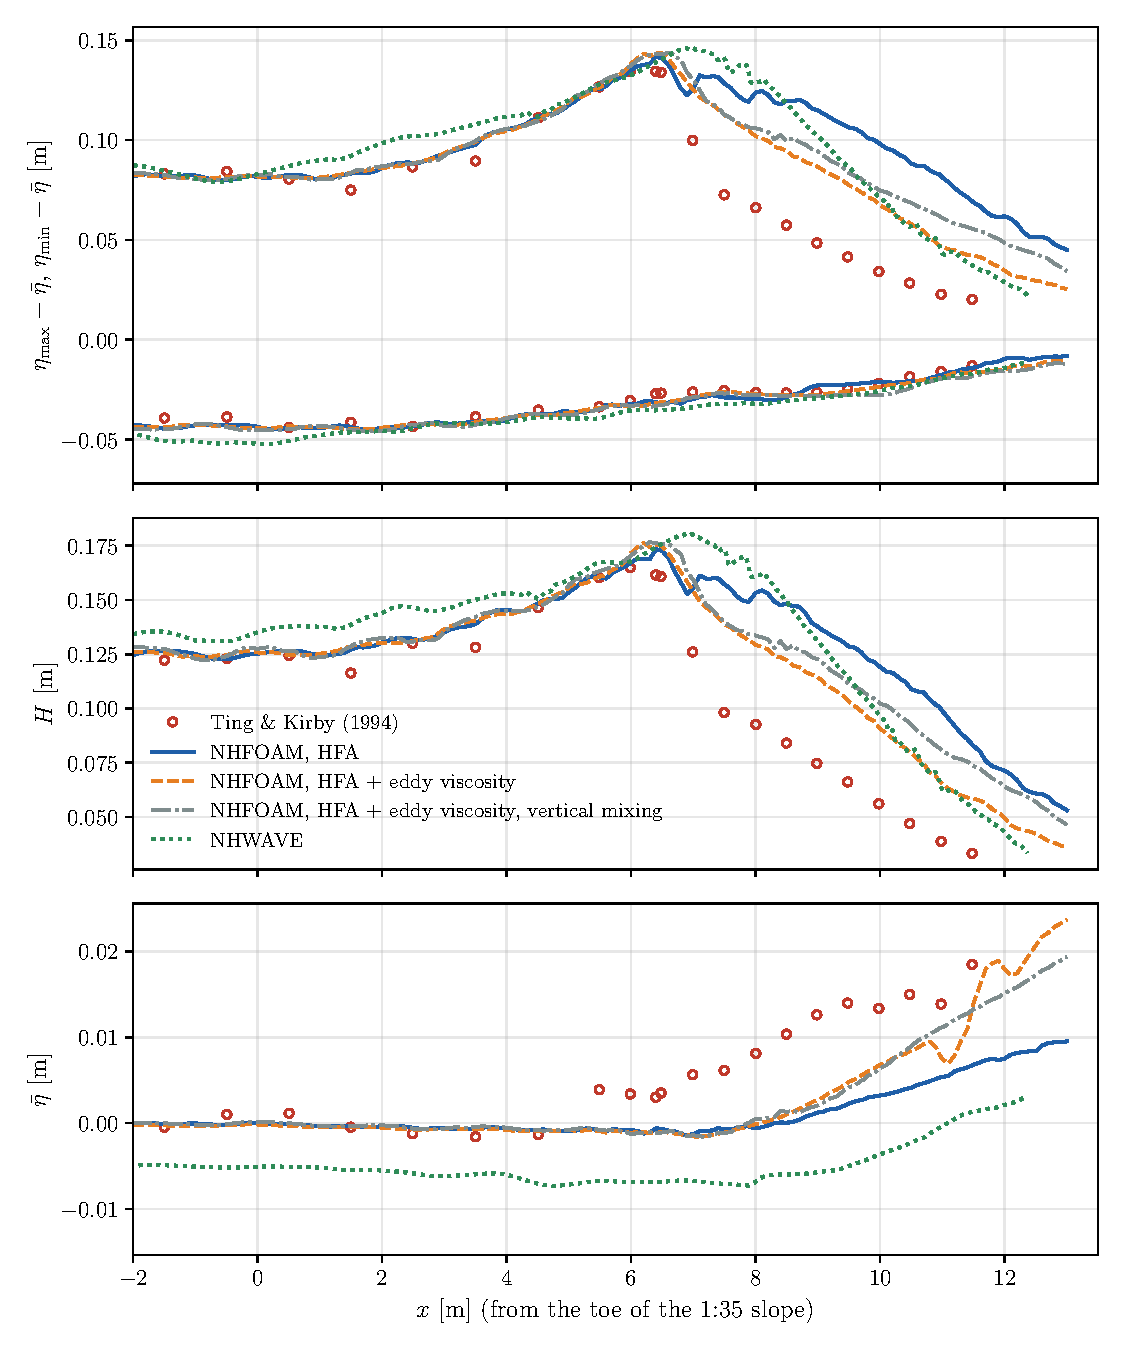
\includegraphics[width=0.9\textwidth]{tk_breaking.pdf}
\caption{Spilling breakers \citep{ting1994} with the breaking models: crest
and trough relative to the mean level, wave height and mean water level.}
\label{fig:brk-tk}
\end{figure}

\begin{figure}[!htbp]
\centering
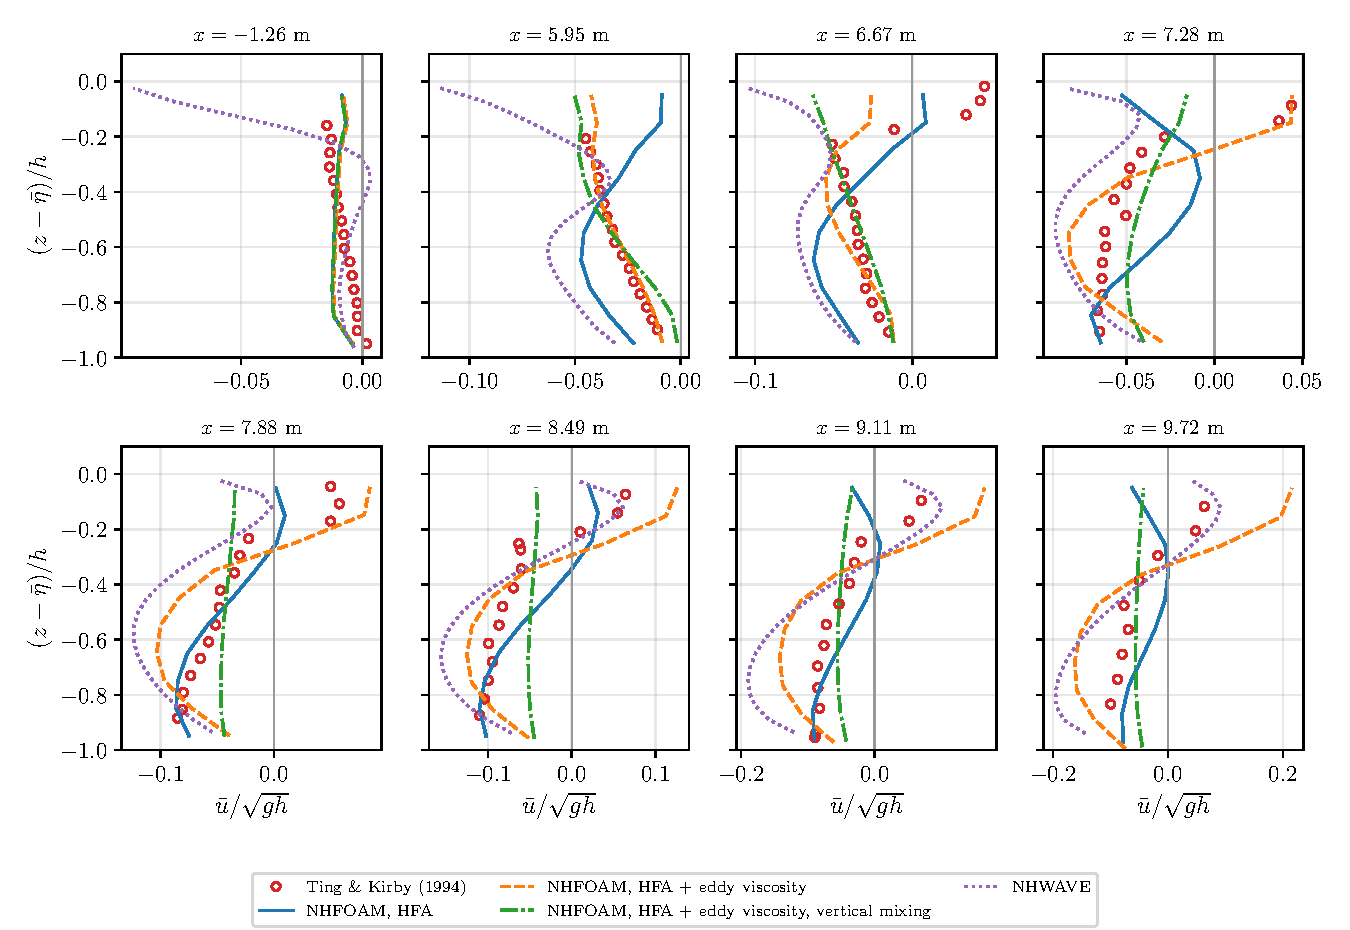
\includegraphics[width=\textwidth]{tk_undertow.pdf}
\caption{Spilling breakers \citep{ting1994}: time-mean horizontal velocity.
The models are averaged at fixed $\sigma$ and plotted at the mean height of
each level; above the trough level ($(z-\bar\eta)/h \gtrsim -0.25$) this is
not the Eulerian mean of the measurements.}
\label{fig:brk-undertow}
\end{figure}

The eddy viscosity makes the difference. With horizontal mixing (the
default), the mean error of the wave height in the surf zone falls from
$+6.1$ cm with the HFA alone to $+3.5$ cm, below NHWAVE's $+4.8$ cm with
$k$--$\epsilon$ and 20 layers, and the mean level near the shoreline rises
towards the measured one (0.8 cm at $x = 11$ m, lab 1.4 cm, HFA 0.5 cm).
The breaking age alone, which lets the hydrostatic region grow over the
face of the bore, changes little ($+5.8$ cm). The eddy viscosity without the HFA ($+4.1$ cm, with vertical mixing)
is close to the hybrid with vertical mixing ($+4.4$ cm): once $\nu_b$ acts,
the hydrostatic front adds little, and the dissipation comes from the eddy
viscosity. Vertical mixing through the layer faces dissipates less and
makes the undertow nearly uniform over the depth, at about 0.65 of the
measured strongest offshore velocity. Without it the profiles keep the
measured shape, onshore near the crests and offshore below, with the
strongest undertow 30\% too large (NHWAVE: 60\%); the HFA alone gives the
right strength but a weaker shear (Fig.~\ref{fig:brk-undertow}). Horizontal
mixing is therefore the default. The kinematic onset with $B_k = 0.85$
breaks 1.1 m late, at a height of 21 cm: with $\sqrt{gD}$ for the crest
speed, the surface velocity reaches $0.85\sqrt{gD}$ only when the wave is
about to overturn. Its smaller mean error inside the surf zone ($+3.1$ cm)
hides the 8 cm overshoot at the breaking point; the criterion needs a better
estimate of the crest speed, for instance from tracking the crests.

All variants keep the same main error, in the transition just after the
breaking point. Between $x = 6.4$ and 8 m the measured height drops from 16.2
to 9.3 cm, that of the models with the eddy viscosity by 4.2--4.6 cm only
(HFA alone 2.0 cm, NHWAVE 1.3 cm); further inshore their decay rates are
close to the measured one (Fig.~\ref{fig:brk-tk}). The eddy
viscosity starts at the onset, but the breaking region covers the face of
the bore only as the breaking event ages ($T^* \approx 0.75$ s at the
breaking point), while the measured breakers lose their height at once. In
a first version, columns joined a breaker at the lower threshold of an old
breaker. In this 2DV case that cut the error of the run with vertical mixing
from $+4.4$ to $+3.5$ cm, but on the beach of Section~\ref{sec:brk-ls} the
breaking region then crept along the crests of the oblique waves into deep
water, where it flagged waves 5 m from the shoreline; columns now join at
$\beta\sqrt{gD}$, the threshold of a new breaker.

On the spilling breakers of \citet{hansen1979} (Section~\ref{sec:breaking};
the same set-up, with the shelf and the velocity-only sponge), the default
nearly halves the error of the wave height in the surf zone, from an rms of 2.98 to
1.54 cm for $x > 8.3$ m ($-19\%$ to $+49\%$ of the measured heights instead of
$+3\%$ to $+99\%$), and that of the mean water level, from 4.6 to 2.2 mm,
with the same error before breaking (0.56 cm). It breaks 0.6 m early, with
the largest height 0.3 cm below the measured one (Fig.~\ref{fig:brk-hs}).

\begin{figure}[!htbp]
\centering
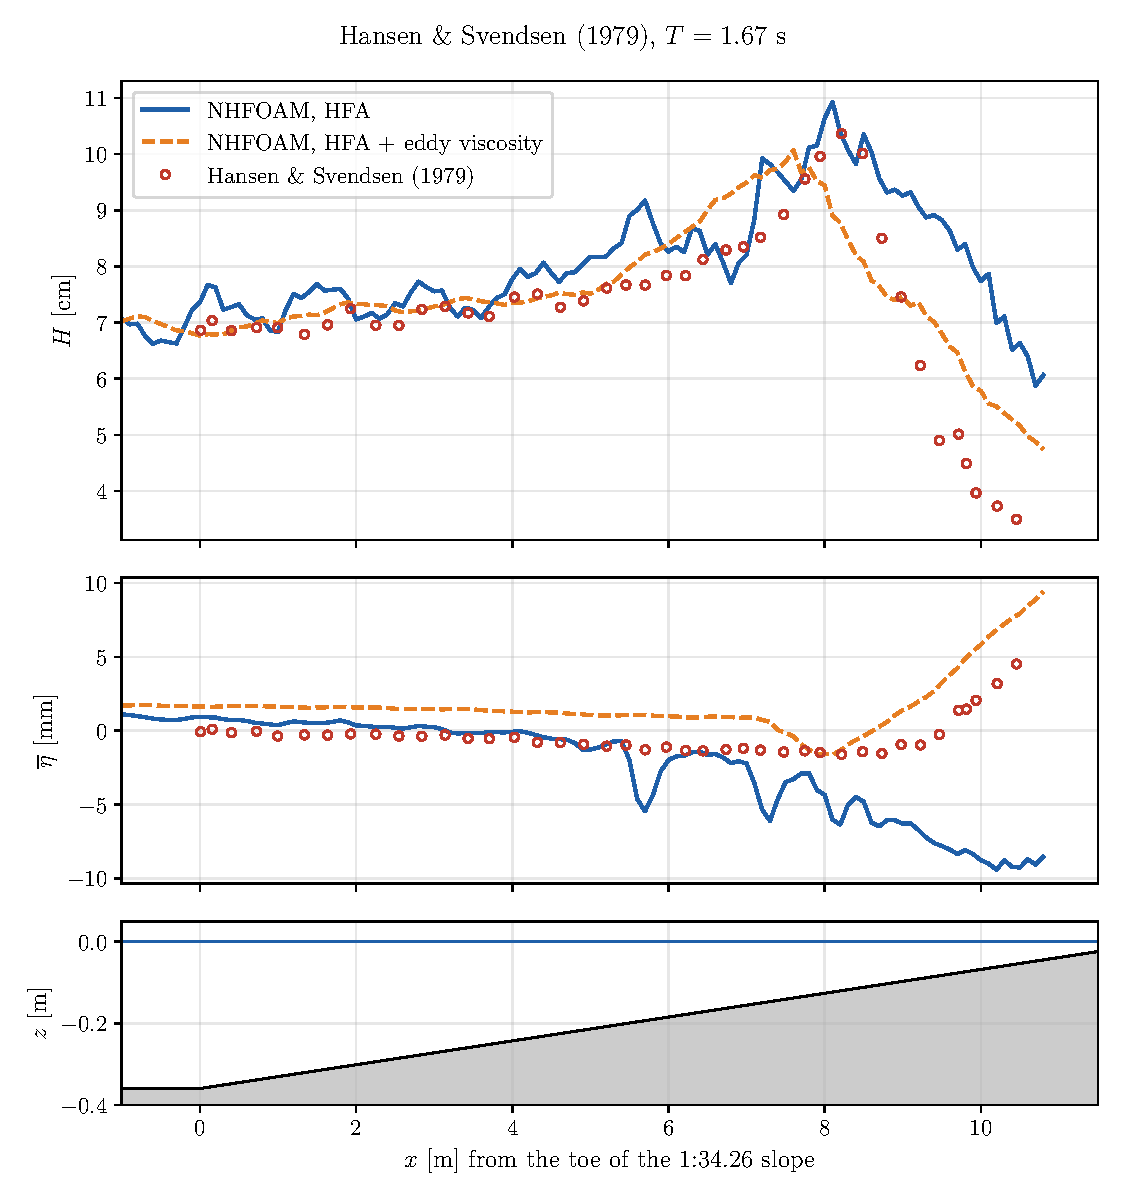
\includegraphics[width=0.85\textwidth]{hs_breaking.pdf}
\caption{Spilling breakers of \citet{hansen1979}: wave height and mean water
level with the HFA and with the default breaking model (HFA and eddy
viscosity).}
\label{fig:brk-hs}
\end{figure}

\subsection{Longshore current on a plane beach}
\label{sec:brk-ls}

\citet{visser1991}, experiment 4, is test 4.7 of \citet{ma2012}: regular
waves, $H = 7.8$ cm and $T = 1.02$ s, arrive at $15.4^\circ$ from the shore
normal over $h = 0.35$ m and break on a smooth concrete beach of slope 1:20,
driving a longshore current. The measurements used here are those tabulated
by \citet{kraus1991}: the wave height, the mean water level and the
depth-averaged longshore current, $(V_s + 2V_m + V_b)/4$ from dye at the
surface, at mid-depth and near the bottom. Visser reports the breaker line
2.51 m and the plunge line 1.92 m from the still-water shoreline, and a
largest current of 0.404 m/s.

Both models are periodic alongshore over one alongshore wavelength,
$L_y = 2\pi/(k\sin\theta)$, and use five uniform layers, log-law friction
with $k_s = 0.8$ mm (the value \citet{ma2012} found by tuning), the
Smagorinsky model with $\Delta = (\Delta x\,\Delta y\,\Delta\sigma D)^{1/3}$
and $C_s = 0.168$, and a 5 mm film; both run for 100 s, and the statistics
use the last five periods (Table~\ref{tab:brk-ls-setup}). \citet{ma2012} ran
NHWAVE on $280\times128$ cells; here both models have the same, coarser
grid, $\Delta x = 4$ cm and 32 (NHWAVE, a power of two for its periodic
boundaries) or 40 (\NHFOAM) cells alongshore, which is the affordable size
on the two cores used for this report. Because the crests are oblique, the
spacing along the wave direction is $\Delta y\sin\theta = 3.7$--4.6 cm, close
to $\Delta x$. \NHFOAM\ runs with the default breaking model of the previous
section, with HFA alone, and with the vertical mixing of the eddy viscosity.

\begin{table}[!htbp]
\centering
\caption{Longshore current: set-up of the two models.}
\label{tab:brk-ls-setup}
\small
\begin{tabular}{lp{5.8cm}p{5.2cm}}
\toprule
 & \NHFOAM & NHWAVE \\
\midrule
domain & 2 m flat (1.5 m wave zone), slope, 0.6 m land & 0.6 m flat, slope, 0.8 m land \\
cells & $240 \times 40 \times 5$, $L_y = 5.600$ m & $210 \times 32 \times 5$, $L_y = 5.533$ m \\
waves & stream function ($N = 24$), relaxation zone & linear, left boundary \\
time step & 10.2 ms (BDF2) & CFL 0.5 (about 9 ms) \\
breaking & HFA + eddy viscosity (or HFA) & shock capturing and Smagorinsky \\
turbulence & Smagorinsky (OpenFOAM LES library) & Smagorinsky (\code{IVTURB = 20}) \\
friction & log law, $k_s = 0.8$ mm & log law, \code{Zob} = 0.8 mm \\
\bottomrule
\end{tabular}
\end{table}

\begin{figure}[!htbp]
\centering
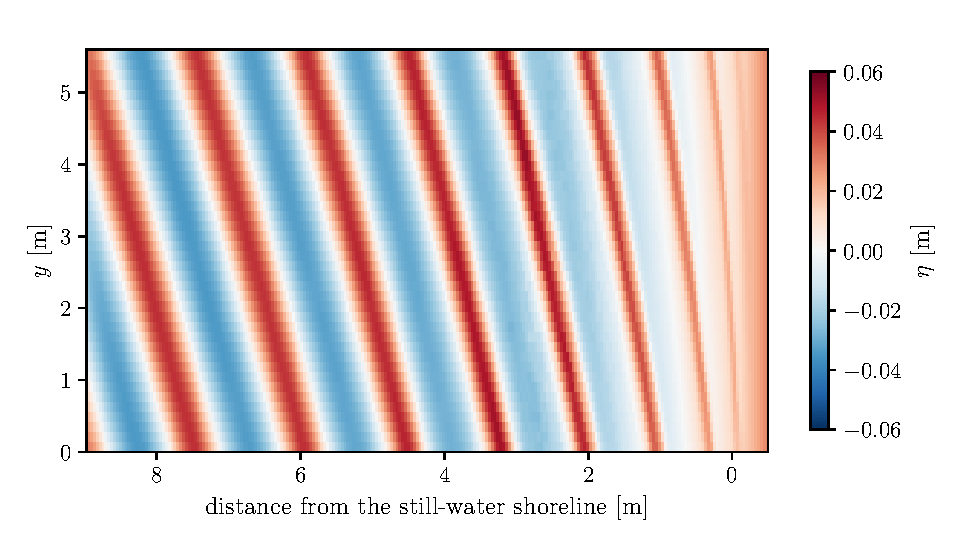
\includegraphics[width=0.8\textwidth]{longshore_snapshot.pdf}
\caption{Longshore current \citep{visser1991}: surface elevation of \NHFOAM\
at $t = 100$ s (default breaking model). The wave zone ends 7.5 m from the
shoreline.}
\label{fig:brk-ls-snap}
\end{figure}

\begin{figure}[!htbp]
\centering
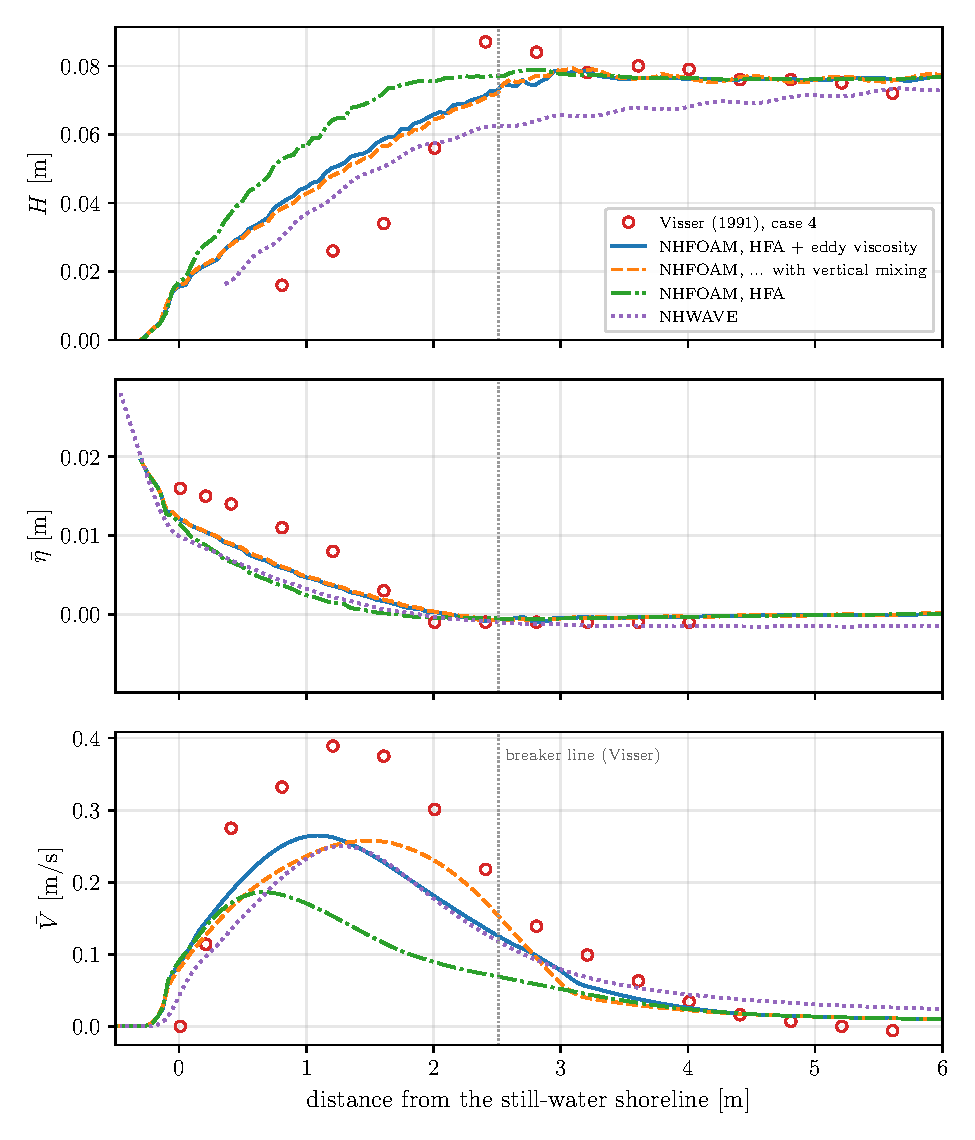
\includegraphics[width=0.85\textwidth]{longshore.pdf}
\caption{Longshore current \citep{visser1991}, case 4: wave height, mean
water level and depth-averaged longshore current, averaged over the last five
periods of 100 s and alongshore. NHWAVE's wave height needs zero crossings
and is not defined in the swash.}
\label{fig:brk-ls}
\end{figure}

\begin{table}[!htbp]
\centering
\caption{Longshore current: wave height at the measured breaking point
(2.41 m from the shoreline) and inside the surf zone (1.21 m), mean water
level at the shoreline, the largest longshore current and its distance from
the shoreline, and rms errors at the measuring stations. \code{hybrid}: HFA
and eddy viscosity (the default).}
\label{tab:brk-ls}
\small
\setlength{\tabcolsep}{4pt}
\begin{tabular}{lcccccc}
\toprule
 & $H$, 2.41 m & $H$, 1.21 m & $\bar\eta$, shore- & largest $\bar V$ & rms error & rms error \\
 & (cm) & (cm) & line (cm) & (m/s), at (m) & $H$ (cm) & $\bar V$ (m/s) \\
\midrule
lab & 8.7 & 2.6 & 1.6 & 0.39, 1.21 & & \\
\NHFOAM, \code{hybrid} & 7.1 & 5.0 & 1.2 & 0.265, 1.08 & 1.3 & 0.074 \\
\quad with vertical mixing & 7.1 & 4.8 & 1.2 & 0.258, 1.48 & 1.2 & 0.071 \\
\NHFOAM, HFA & 7.7 & 6.4 & 1.1 & 0.186, 0.68 & 1.9 & 0.123 \\
NHWAVE & 6.2 & 4.2 & 0.7 & 0.250, 1.26 & 1.3 & 0.082 \\
\bottomrule
\end{tabular}
\end{table}

The crests turn towards the shore over the slope (Fig.~\ref{fig:brk-ls-snap}).
In \NHFOAM\ the waves start breaking about 2.85 m from the shoreline, 0.35 m
seaward of Visser's breaker line, at 7.9 cm instead of the measured 8.7 cm,
and inside the surf zone their heights stay above the measured ones, as on
the two 2DV beaches (Fig.~\ref{fig:brk-ls}, Table~\ref{tab:brk-ls}). The
set-up at the shoreline is 1.2 cm (lab 1.6 cm). NHWAVE's waves lose height
on this grid before they break, from 7.9 cm at the wavemaker to 6.2 cm at
the measured breaking point.

Both models put the longshore current in about the right place but give two
thirds of its strength: 0.265 m/s at 1.08 m from the shoreline (\NHFOAM) and
0.250 m/s at 1.26 m (NHWAVE), against 0.39 m/s at 1.21 m. With the HFA alone
the waves keep more of their height inside the surf zone, and the current is
weaker, 0.19 m/s, with its peak at 0.68 m, close to the shoreline: the
behaviour \citet{ma2012} found when they switched off the turbulent
diffusion. The breaking eddy viscosity mixes the current across the surf
zone as well as dissipating the waves; with vertical mixing as well the peak
moves to 1.48 m. The current is uniform alongshore (over the columns at one
cross-shore position, the standard deviation of the mean depth-averaged
current is below 0.003 m/s), the mean
cross-shore velocity is an undertow of up to 4.6 cm/s, and the current still
builds up slowly: its peak grew by 2\% between 90 and 100 s.

\citet{ma2012} report the current well predicted by NHWAVE on their finer grid
($\Delta x = 3$ cm, $\Delta y$ three to four times smaller than here), so the
resolution of this grid is the likely main cause of the deficit both models
share; in \NHFOAM\ the slow decay of the heights after breaking also spreads
the forcing over a wider surf zone. On this grid each model took about 70 min
on one core (\NHFOAM: 48\,000 cells and 9800 steps; NHWAVE: 33\,600 cells);
the finer grid would take several hours on the two cores used here and is
left for a later run.

\FloatBarrier
\section{Wave input, unstructured meshes and robustness}
\label{sec:ext}

This section tests what was added after the comparisons with NHWAVE: the
boundary wavemaker with active absorption, the return current, irregular
waves and measured records (Section~\ref{sec:zones}), with the composite
beach of NTHMP benchmark 5, the model on triangulated meshes, and the
checks that keep the code reproducible: parallel runs, restarts and a
regression suite.

\subsection{Boundary wavemaker and active absorption}
\label{sec:wm}

The tests (script \code{wavemaker.py}) use a flat flume ($h = 0.4$ m,
10 layers, $\Delta x = 2$ cm, $\Delta t = 10$ ms) with regular waves of
$H = 2$ cm and $T = 1.5$ s ($kh = 0.96$) unless stated otherwise. Incident
and reflected amplitudes come from a least-squares fit of
$A_j = a_I e^{ikx_j} + a_R e^{-ikx_j}$ to the first harmonic at 30--70
gauges \citep{zelt1992}, with $k$ adjusted to the model's own wave number
(within 0.1\% of linear theory in the runs of progressive waves).

\paragraph{Progressive waves.} With the wavemaker at $x = 0$ and a 6 m
sponge at the far end, the wave height is within 0.7\% of the target over
13.5 m (mean $0.995H$), and the reflection coefficient of the flume is
0.4\%. A 6 m relaxation zone (2.3 wavelengths) gives $0.998H$ and 0.16\%
(Fig.~\ref{fig:wm-reg}a), with a domain 6 m longer.

\paragraph{Closed flume.} With a wall 10 m from the wavemaker, the waves
reflected by the wall return to the wavemaker. With active absorption the
incident amplitude settles at $1.03\,a$ within 5 periods and stays there for
the 60 periods of the run, with a standing wave of $a_R/a_I = 0.99$ in
front of the wall. Without absorption the wavemaker reflects the returning
waves, which beat with the generated ones: the incident amplitude swings
between $0.1\,a$ and $1.1\,a$ with a period of about 40 s
(Fig.~\ref{fig:wm-reg}b). The 3\% excess with absorption is the
re-reflection of the shallow-water absorber at this $kh$ (below).

\paragraph{Absorbing boundary.} The same condition with zero wave height
lets waves out of the domain. Regular waves made by a 6 m relaxation zone
and absorbed 8 m further on give the reflection coefficients of
Table~\ref{tab:wm-abs} and Fig.~\ref{fig:wm-abs}. With the shallow-water
celerity the reflection follows the estimate
$(1 - c/\sqrt{gh})/(1 + c/\sqrt{gh})$, the mismatch between the imposed
depth-averaged velocity $\sqrt{g/h}\,\eta$ and that of the wave,
$c\,\eta/h$: 1.9\% at $kh = 0.53$, 5.9\% at 0.96 and 12.6\% at 1.72. With
the phase speed of the waves (\code{absorptionCelerity wave}) the
depth-averaged velocity matches, and the reflection falls to 0.3\% and
1.7\% for $kh \le 1$; for shorter waves a correction that is uniform over
the depth cannot match the profile of the wave (9.3\% at $kh = 1.72$). A
sponge layer of 2--5 wavelengths reflects less than 0.5\%, at the cost of
the domain.

\begin{table}[!htbp]
\centering
\caption{Reflection coefficient of the absorbing boundary and of an 8 m
sponge layer, regular waves of $H = 2$ cm in $h = 0.4$ m.}
\label{tab:wm-abs}
\small
\begin{tabular}{ccccc}
\toprule
$T$ & $kh$ & \code{absorptionCelerity shallow} & \code{absorptionCelerity wave} & 8 m sponge \\
\midrule
2.5 s & 0.53 & 1.9\% & 0.3\% & 0.2\% \\
1.5 s & 0.96 & 5.9\% & 1.7\% & 0.4\% \\
1.0 s & 1.72 & 12.6\% & 9.3\% & $<0.1$\% \\
\bottomrule
\end{tabular}
\end{table}

\paragraph{Return current.} In a closed flume of constant depth (a 6 m
wave-making zone, a wall 10 m further on) the mean water level of the flume
stays within 0.1 mm of still water with or without the return current
(Fig.~\ref{fig:wm-reg}c), and within 0.2 mm with the boundary wavemaker and
absorption: the zone relaxes the surface to the target, so the missing
return current only steps the mean level inside the zone. Over the
submerged bar it matters (Section~\ref{sec:bar-bc}).

\begin{figure}[!htbp]
\centering
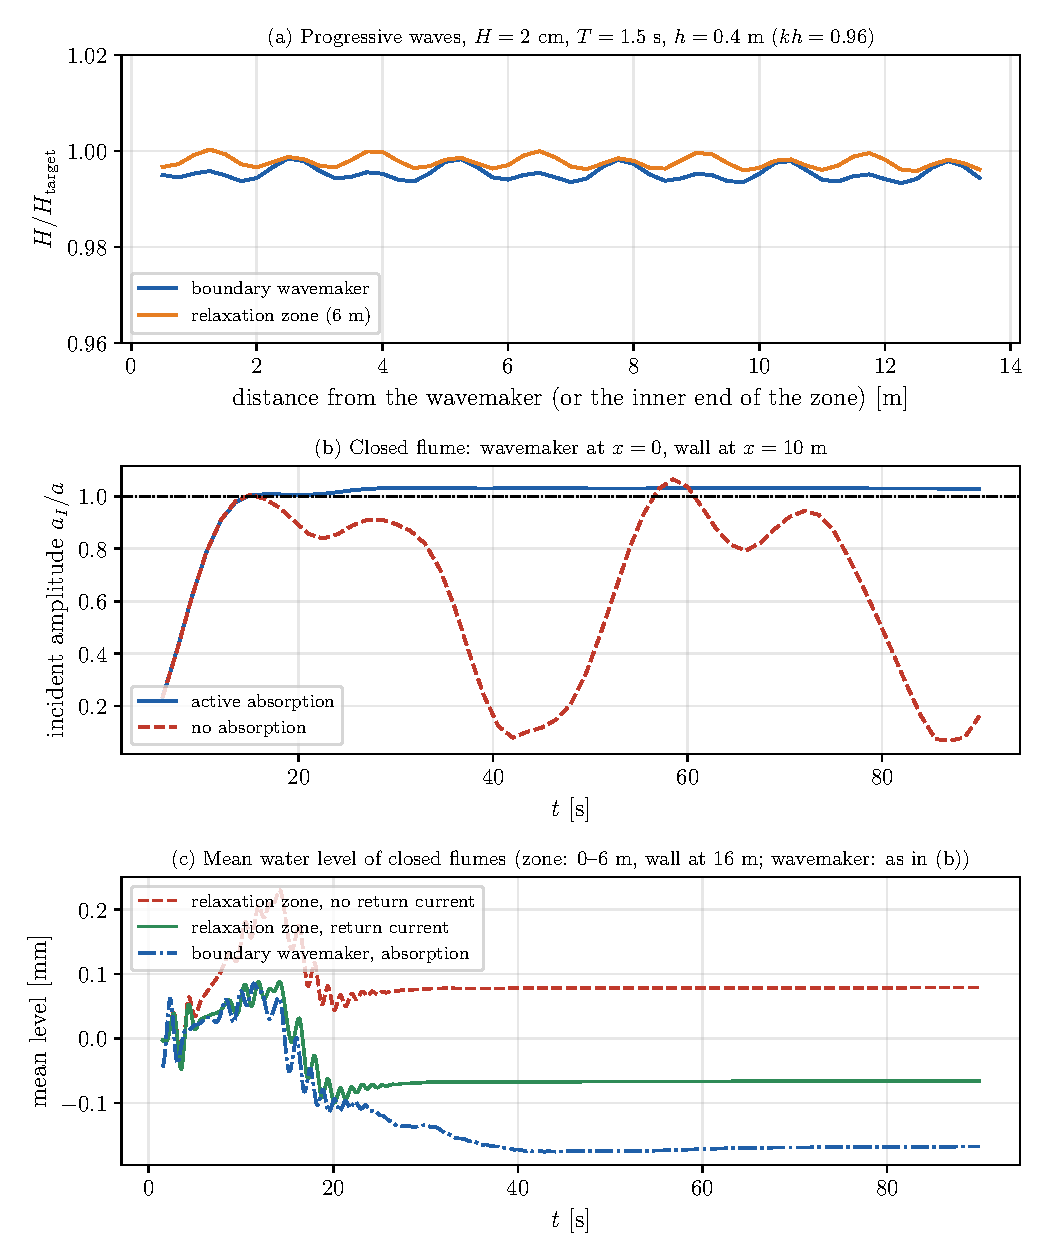
\includegraphics[width=0.85\textwidth]{wavemaker_regular.pdf}
\caption{Wave input in a flat flume ($h = 0.4$ m, $H = 2$ cm, $T = 1.5$ s):
(a) wave height from the boundary wavemaker and from a relaxation zone;
(b) incident amplitude in a closed 10 m flume with and without active
absorption; (c) the mean water level of closed flumes with a relaxation
zone (with and without the return current) and with the wavemaker of (b).}
\label{fig:wm-reg}
\end{figure}

\begin{figure}[!htbp]
\centering
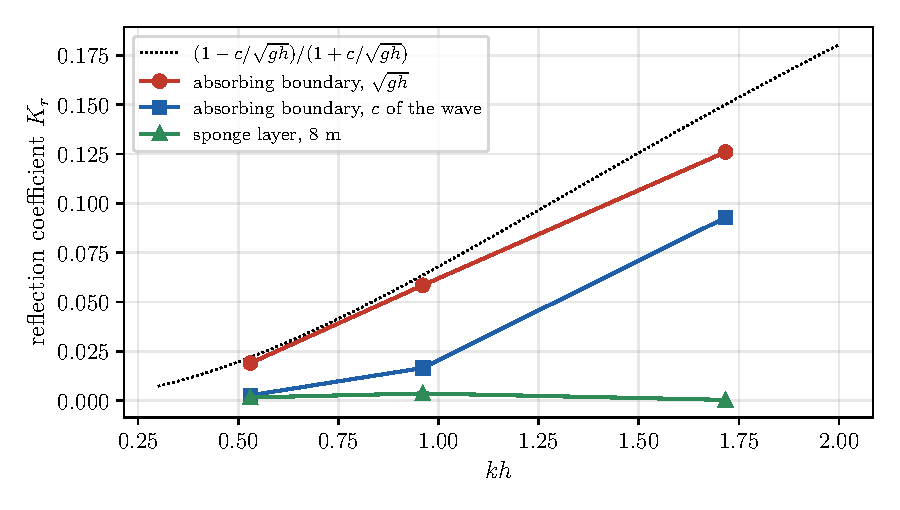
\includegraphics[width=0.65\textwidth]{wavemaker_absorber.pdf}
\caption{Reflection coefficient of the absorbing boundary (\code{nhWaveVelocity}
with zero wave height) with the shallow-water celerity and with the phase
speed of the waves, and of an 8 m sponge layer; the dotted line is the
depth-averaged estimate for the shallow-water absorber.}
\label{fig:wm-abs}
\end{figure}

\subsection{Irregular waves}
\label{sec:irr}

JONSWAP waves ($H_s = 3$ cm, $T_p = 1.5$ s, $\gamma = 3.3$, 100 components
between $0.5f_p$ and $3f_p$, random phases) were made in the same flume by a
6 m relaxation zone and by the boundary wavemaker, and the spectra were
computed at six gauges over 200 s (Welch, 40 s segments;
Fig.~\ref{fig:wm-irr}). Both keep the shape of the target spectrum and its
peak period (1.47 s, the frequency resolution of the spectra), and $H_{m0}$
stays within $-4\%$ and $+2\%$ of the target over 12 m (8 peak
wavelengths). In all runs $H_{m0}$ falls by 3--5\% between 2 and 12 m from
the generator. The loss is in the peak band (0.6--0.75 Hz: 18\% of its
energy over 10 m), it is the same with filtered central convection as with
the TVD scheme, and regular waves of the peak period and 2 cm height do
not show it; its cause is not yet identified.

\begin{figure}[!htbp]
\centering
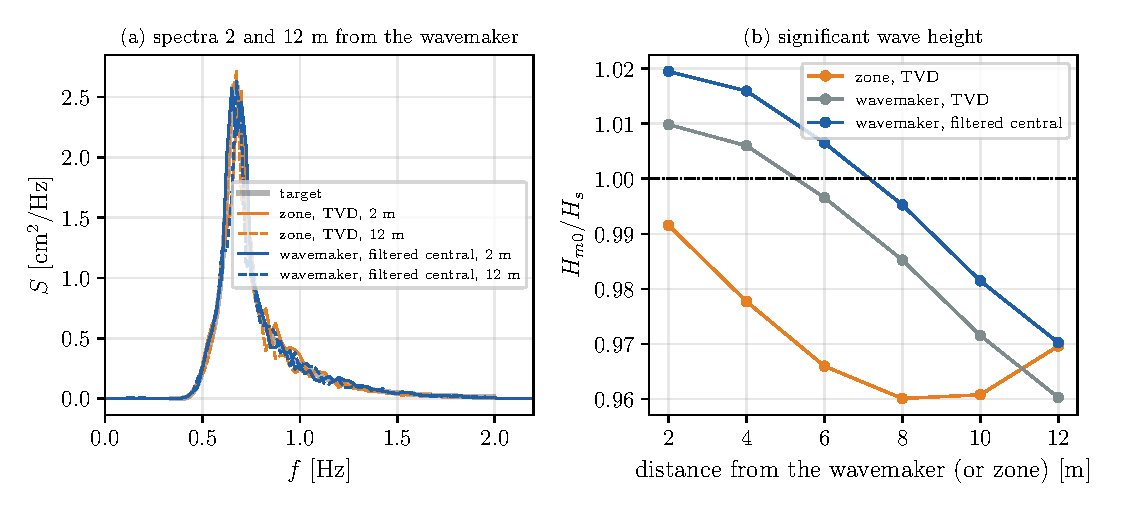
\includegraphics[width=\textwidth]{wavemaker_irregular.pdf}
\caption{JONSWAP waves ($H_s = 3$ cm, $T_p = 1.5$ s, $\gamma = 3.3$, 100
components) from a relaxation zone and from the boundary wavemaker:
(a) spectra 2 and 12 m from the generator against the target; (b) $H_{m0}$
along the flume.}
\label{fig:wm-irr}
\end{figure}

\subsection{The submerged bar: return current and long waves}
\label{sec:bar-bc}

In case C of the submerged bar (Section~\ref{sec:bar10}) the phase of the
waves over the bar drifted during the run, and with it the rms error
(Table~\ref{tab:barwindow}). The case was rerun on the same mesh with the
8 m wave-making zone and the return current, and with the boundary
wavemaker at $x = 0$ (active absorption and return current) in place of
the zone (Table~\ref{tab:bar-bc}, Fig.~\ref{fig:bar-bc}).

\begin{table}[!htbp]
\centering
\caption{Submerged bar, case C, 10 layers: rms error over the 10 gauges for
windows ending at 45--65 s, the time lag of the first harmonic at
$x = 35.7$ m behind $x = 22$ m from the window ending at 45 s to that
ending at 65 s (NHWAVE: 60 s), and the spread of the mean water level over
the gauges.}
\label{tab:bar-bc}
\small
\setlength{\tabcolsep}{3.5pt}
\begin{tabular}{lccccccc}
\toprule
 & \multicolumn{5}{c}{rms error (cm), window ending at} & lag (s) & mean level \\
\cmidrule(lr){2-6}
 & 45 s & 50 s & 55 s & 60 s & 65 s & 45 $\to$ 65 s & spread (mm) \\
\midrule
zone, no return current (Sec.~\ref{sec:bar10}) & 0.49 & 0.65 & 0.94 & 1.18 & 1.39 & $0.98 \to 1.19$ & 1.9--3.6 \\
zone, return current & 1.03 & 1.01 & 1.00 & 1.00 & 1.03 & $0.83 \to 0.84$ & 0.7--0.8 \\
boundary wavemaker & 0.90 & 0.99 & 1.00 & 0.98 & 0.98 & $0.86 \to 0.85$ & 0.7--2.5 \\
NHWAVE & 1.08 & 1.02 & 0.97 & 0.89 & 0.77 & $0.80 \to 0.84$ & 0.9--2.1 \\
REEF3D::NHFLOW & 0.93 & 0.92 & 0.92 & 0.98 & 1.10 & $0.85 \to 0.78$ & 0.9--1.6 \\
lab & & & & & & 0.96 & \\
\bottomrule
\end{tabular}
\end{table}

The drift came from the missing return current. A wave-making zone without
it imposes no mean flow, while the waves carry the Stokes transport into the
closed flume, which must return as a mean current; the mismatch drives mean
currents and long waves, which shift the waves over the 0.1 m deep crest.
With the return current, in the zone or at the wavemaker, the lag no longer
drifts (0.01 s in 20 s instead of 0.21 s), the mean water level varies by
less than 1 mm along the flume once the wave train has passed, and the
error is about 1.0 cm in every window. \NHFOAM\ then has the waves 0.12 s
early at $x = 35.7$ m, like NHWAVE and REEF3D::NHFLOW (0.1--0.18 s); the
smaller errors of the run without the return current in short windows came
from the drift passing through the measured phase. The test of a closed
flume of constant depth (Fig.~\ref{fig:wm-reg}c) is not sensitive to the
return current, because there the mismatch only steps the mean level inside
the zone, by a fraction of a millimetre.

\begin{figure}[!htbp]
\centering
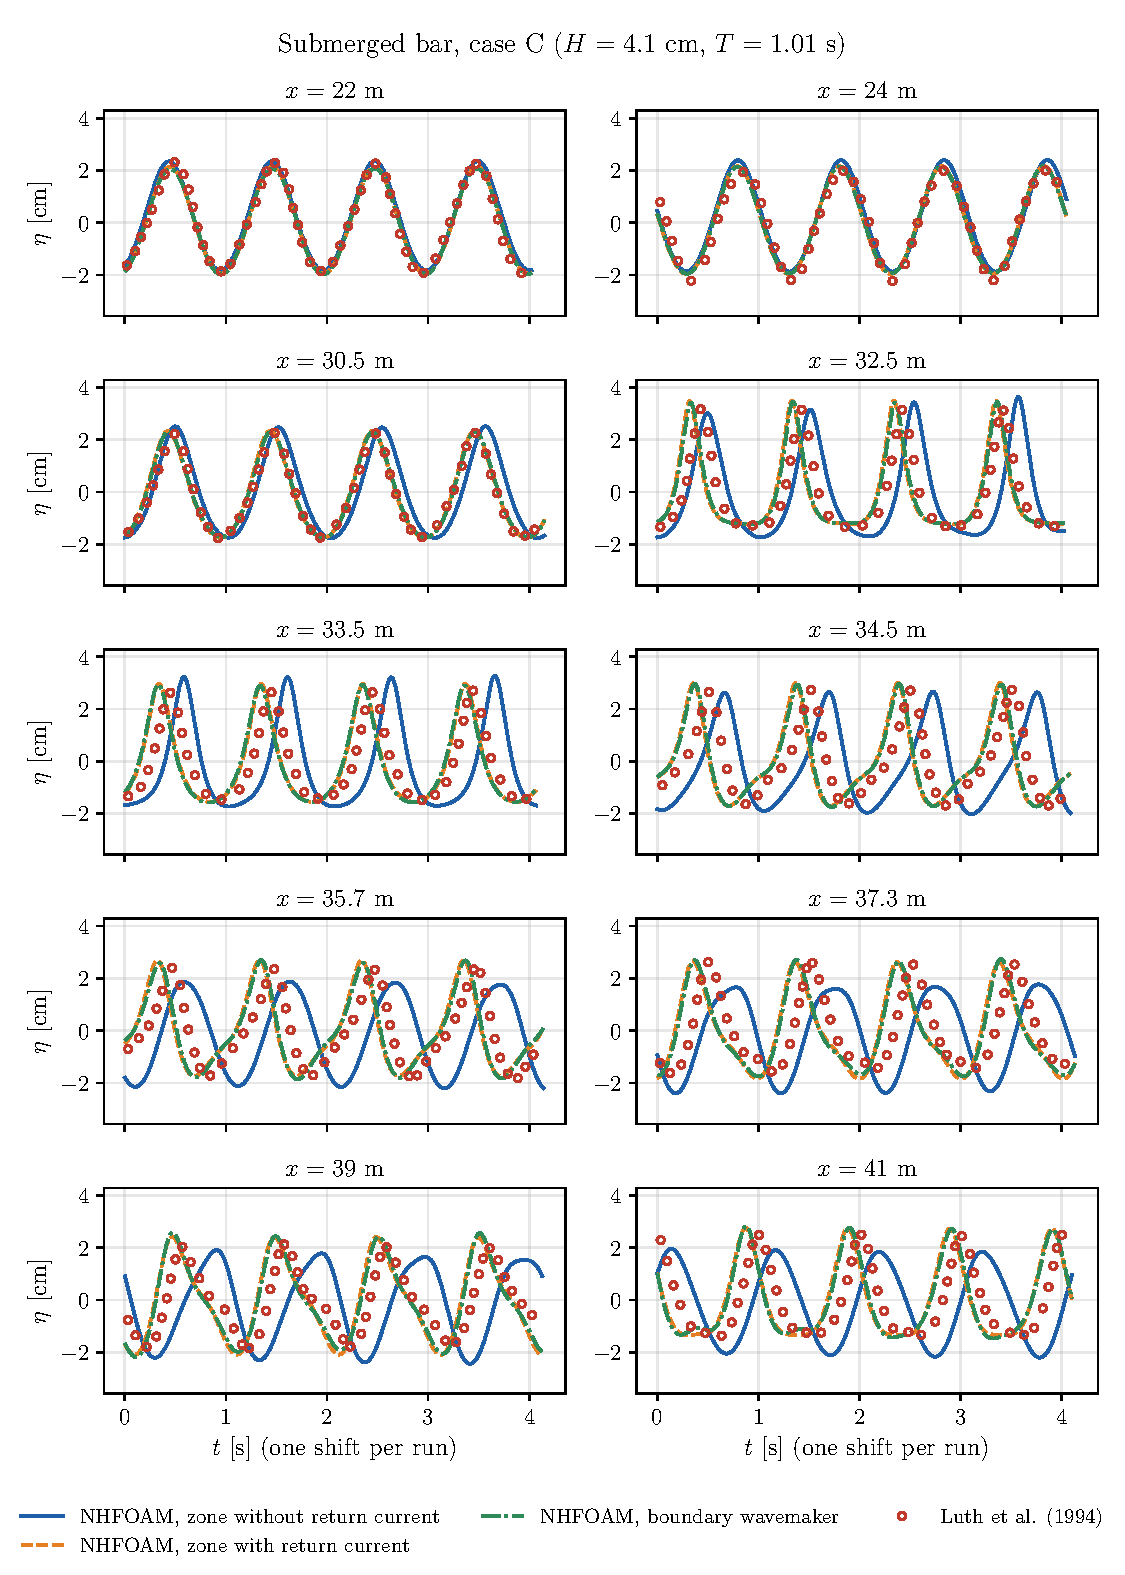
\includegraphics[width=0.9\textwidth]{bar_bc_C.pdf}
\caption{Submerged bar, case C, 10 layers, window ending at 65 s: the
wave-making zone without and with the return current, and the boundary
wavemaker, against \citet{luth1994}.}
\label{fig:bar-bc}
\end{figure}

\subsection{Measured records}
\label{sec:ts}

The time-series input \eqref{eq:timeseries} was first checked on a wave
whose answer is known (script \code{timeseries\_input.py}): a solitary wave
of $H/h = 0.1$, 0.3 and 0.6 is made at $x = 0$ of a flat tank ($h = 0.218$ m,
$\Delta x = 2$ cm, 5 layers, $\Delta t = 5$ ms, a 3 m sponge at the far end)
from its own record, sampled every 0.02 s like a gauge, and compared 12 m
downstream with the exact wave of Babenko's equation. The elevation record
runs with the active absorption, the paddle record (the time integral of
$c\,\eta/(h+\eta)$) without it; for reference the same wave also starts as
the exact initial condition (Table~\ref{tab:ts}, Fig.~\ref{fig:ts}).

\begin{table}[!htbp]
\centering
\caption{Solitary wave made from its record at $x = 0$, 12 m downstream:
crest height, arrival of the crest and rms difference over the pulse
against the exact wave.}
\label{tab:ts}
\small
\begin{tabular}{llccc}
\toprule
$H/h$ & input & crest$/H$ & arrival & rms$/H$ \\
\midrule
0.1 & exact initial condition & 1.000 & $-9$ ms & 0.4\% \\
0.1 & elevation, $c = \sqrt{g(h+\eta)}$ & 0.993 & $-2$ ms & 0.3\% \\
0.1 & elevation, $c$ of the wave & 0.997 & $-7$ ms & 0.3\% \\
0.1 & paddle & 1.000 & $-9$ ms & 0.4\% \\
\midrule
0.3 & exact initial condition & 0.997 & $-6$ ms & 0.6\% \\
0.3 & elevation, $c = \sqrt{g(h+\eta)}$ & 0.979 & $+17$ ms & 1.8\% \\
0.3 & elevation, $c$ of the wave & 0.995 & $-3$ ms & 0.3\% \\
0.3 & paddle & 0.996 & $-3$ ms & 0.2\% \\
\midrule
0.6 & exact initial condition & 0.980 & $+3$ ms & 0.5\% \\
0.6 & elevation, $c = \sqrt{g(h+\eta)}$ & 0.991 & 0 ms & 0.5\% \\
0.6 & elevation, $c$ of the wave & 1.037 & $-58$ ms & 9.5\% \\
0.6 & paddle & 0.937 & $+56$ ms & 8.1\% \\
\bottomrule
\end{tabular}
\end{table}

Up to $H/h = 0.3$ the input with the celerity of the wave, and the paddle
record, are as good as the exact initial condition: crests within 0.5\% of
$H$, arrival within 10 ms after 12 m, trailing waves below 0.1\%
($H/h = 0.1$) and 0.7\% of $H$ ($H/h = 0.3$). The local celerity
$\sqrt{g(h+\eta)}$ of the NTHMP benchmarks carries too little water on the
flanks of the pulse, so the wave of $H/h = 0.3$ comes out 2\% low and 17 ms
late. At $H/h = 0.6$ (with $\Delta t = 4$ ms) a velocity that is uniform
over the depth no longer fills the boundary column under the steep crest:
the paddle record, without absorption, makes the wave 6\% low and 56 ms
late, and with an elevation record the active absorption makes up the
difference, too much with the celerity of the wave (4\% high, 58 ms early)
and about right with the local celerity (1\% low, on time). The local
celerity is therefore the safer choice for steep pulses, and
$\sqrt{g(h+H)}$ the better one for $H/h \le 0.3$.

\begin{figure}[!htbp]
\centering
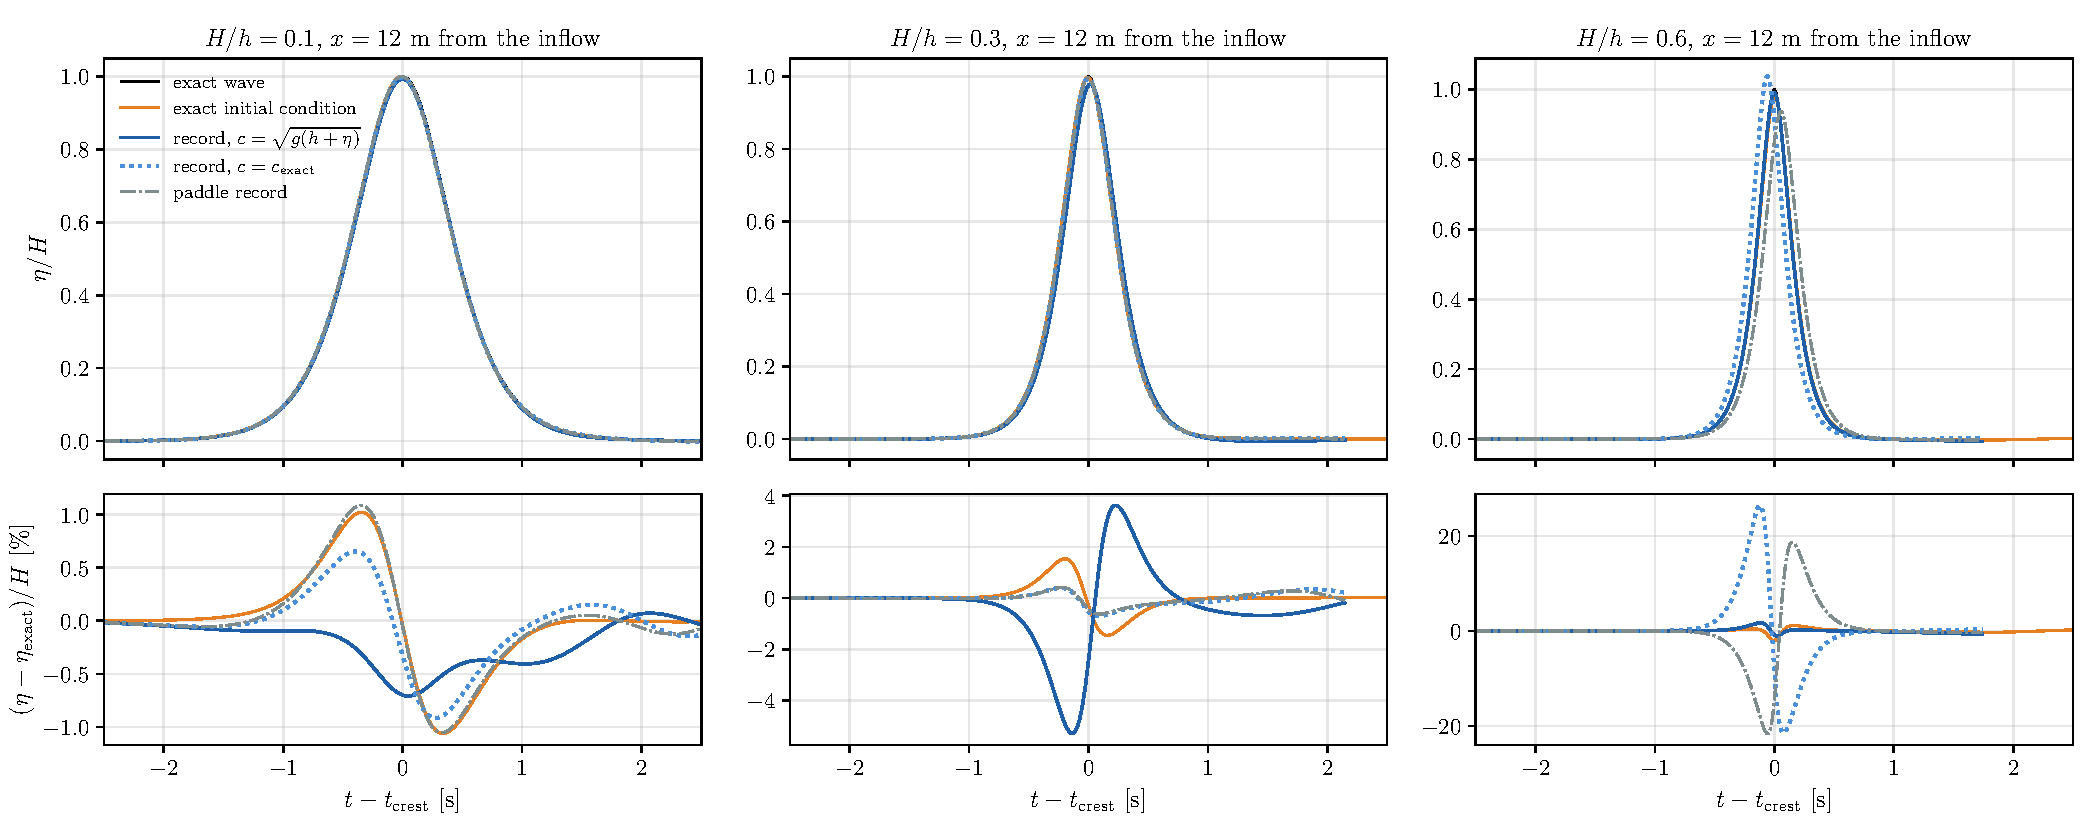
\includegraphics[width=\textwidth]{timeseries_input.pdf}
\caption{Solitary waves made from their records at $x = 0$, 12 m
downstream, against the exact wave: elevation (top) and difference from the
exact wave (bottom).}
\label{fig:ts}
\end{figure}

\subsection{Solitary waves on a composite beach with a vertical wall}
\label{sec:cb}

The Coastal and Hydraulics Laboratory of the US Army Corps of Engineers
built a model of Revere Beach in a flume: 0.218 m of water from the
wavemaker to 15.04 m, then slopes of 1:53, 1:150 and 1:13 up to a vertical
wall at 23.23 m that stands in 4.7 cm of water (benchmark problem 3 of the
1995 long-wave run-up workshop, \citealp{yeh1996}; NTHMP benchmark 5;
\citealp{kanoglu1998} give its linear solution). It is one of the tests of
NHWAVE's tsunami benchmark report \citep{tehranirad2012}. Solitary waves of
target $H/d = 0.05$, 0.30 and 0.70 (cases A, B and C; 0.038, 0.26 and 0.68
at the incident gauge 4) shoal over the slopes, reflect from the wall (B and
C break first) and run back past gauges 4--10, and the highest run-up on
the wall was measured. The benchmark gives the paddle trajectories and
recommends driving the models with the record of gauge 4, which is what the
time-series input is for (script \code{composite\_beach.py}).

Both models use 3 layers, log-law friction with $k_s = 0.1$ mm (NHWAVE's
\code{Zob} in its examples of the inundation benchmarks) and a 5 mm film;
\NHFOAM\ runs its hybrid breaking model. \NHFOAM\ makes the wave in three
ways on a 1 cm grid, the grid of NHWAVE's report: from the record of gauge 4
(the domain starts at the gauge, and the direct pulse, to 275 s, drives
\code{nhWaveVelocity} with the benchmark's velocity relation and the
active absorption), from the paddle record (the whole flume, from the middle
of the paddle stroke, without absorption), and as the exact solitary wave of
the height measured at gauge 4, its crest timed to the measured one there.
The last is also NHWAVE's input. On the 1 cm grid NHWAVE grows short-wave
noise in this flume (wiggles of $\pm1.5$ mm on the 8 mm crest of case A,
crests 3--8\% high, with or without its $k$--$\varepsilon$ model, in a flat
tank as well), so the two models are compared on a 2 cm grid, where NHWAVE
carries the solitary wave cleanly. NHWAVE's $k$--$\varepsilon$ model, on in
its inundation examples, damps the steep waves of cases B and C already on
the flat bed (in a flat tank a wave of $H/d = 0.26$ keeps $0.87H$ after
3.5 m with it and $1.02H$ without it), so NHWAVE runs without it and, for
reference, with it. Table~\ref{tab:cb} and Fig.~\ref{fig:cb} compare the
runs with the measurements; no run is shifted in time.

\begin{table}[!htbp]
\centering
\caption{Composite beach: crests against the measured ones (model/lab $-$ 1,
\%): the incident crest at gauges 4, 5, 7 and 8 (at gauge 4 of the record
run the boundary column against the record), the highest crest at gauges 9
and 10, where the incident and reflected waves overlap, and the reflected
crest at gauge 5; the rms difference over gauges 5--10 from the arrival of
the wave; the highest water level $R$ at the wall. Gauge 10 saturated in
case B.}
\label{tab:cb}
\small
\setlength{\tabcolsep}{3pt}
\begin{tabular}{llrrrrrrrcc}
\toprule
case & run & g4 & g5 & g7 & g8 & g9 & g10 & g5 refl. & rms (cm) & $R$ (cm) \\
\midrule
A & lab & & & & & &  & & & 2.74 \\
A & \NHFOAM, gauge 4 record & 0 & $-$5 & $-$5 & +3 & $-$4 & $-$10 & +10 & 0.08 & 2.30 \\
A & \NHFOAM, paddle record & +27 & +16 & +15 & +25 & +25 & +19 & +40 & 0.19 & 2.76 \\
A & \NHFOAM, solitary, 2 cm & 0 & $-$9 & $-$9 & $-$2 & $-$1 & $-$2 & +8 & 0.11 & 2.13 \\
A & NHWAVE, solitary, 2 cm & +1 & $-$8 & $-$9 & $-$1 & +1 & $-$1 & +14 & 0.11 & 2.16 \\
A & NHWAVE $k$--$\varepsilon$, 2 cm & +1 & $-$8 & $-$9 & $-$1 & +3 & $-$1 & +13 & 0.11 & 2.19 \\
\midrule
B & lab & & & & & & (clipped) & & & 45.7 \\
B & \NHFOAM, gauge 4 record & $-$1 & +10 & $-$7 & $-$1 & +7 &  & +16 & 0.63 & 17.4 \\
B & \NHFOAM, paddle record & +15 & +22 & +7 & +15 & +26 &  & +27 & 1.12 & 18.6 \\
B & \NHFOAM, solitary, 2 cm & $-$1 & +5 & $-$9 & $-$3 & +5 &  & +19 & 0.75 & 18.8 \\
B & NHWAVE, solitary, 2 cm & +5 & +11 & $-$8 & $-$5 & +5 &  & +25 & 0.90 & 19.6 \\
B & NHWAVE $k$--$\varepsilon$, 2 cm & $-$21 & $-$15 & $-$26 & $-$23 & $-$2 &  & $-$7 & 0.27 & 17.5 \\
\midrule
C & lab & & & & & &  & & & 27.4 \\
C & \NHFOAM, gauge 4 record & $-$14 & +12 & $-$18 & +46 & +30 & $-$12 & +27 & 1.34 & 23.8 \\
C & \NHFOAM, paddle record & +7 & +15 & $-$18 & +46 & +28 & $-$12 & +29 & 1.90 & 23.5 \\
C & \NHFOAM, solitary, 2 cm & $-$7 & 0 & $-$17 & +39 & +29 & $-$16 & +20 & 1.08 & 23.6 \\
C & NHWAVE, solitary, 2 cm & $-$20 & +1 & $-$14 & +75 & +34 & $-$11 & +13 & 1.17 & 28.4 \\
C & NHWAVE $k$--$\varepsilon$, 2 cm & $-$21 & $-$15 & $-$15 & +71 & +21 & $-$17 & $-$5 & 0.92 & 24.7 \\
\bottomrule
\end{tabular}
\end{table}

\begin{figure}[!htbp]
\centering
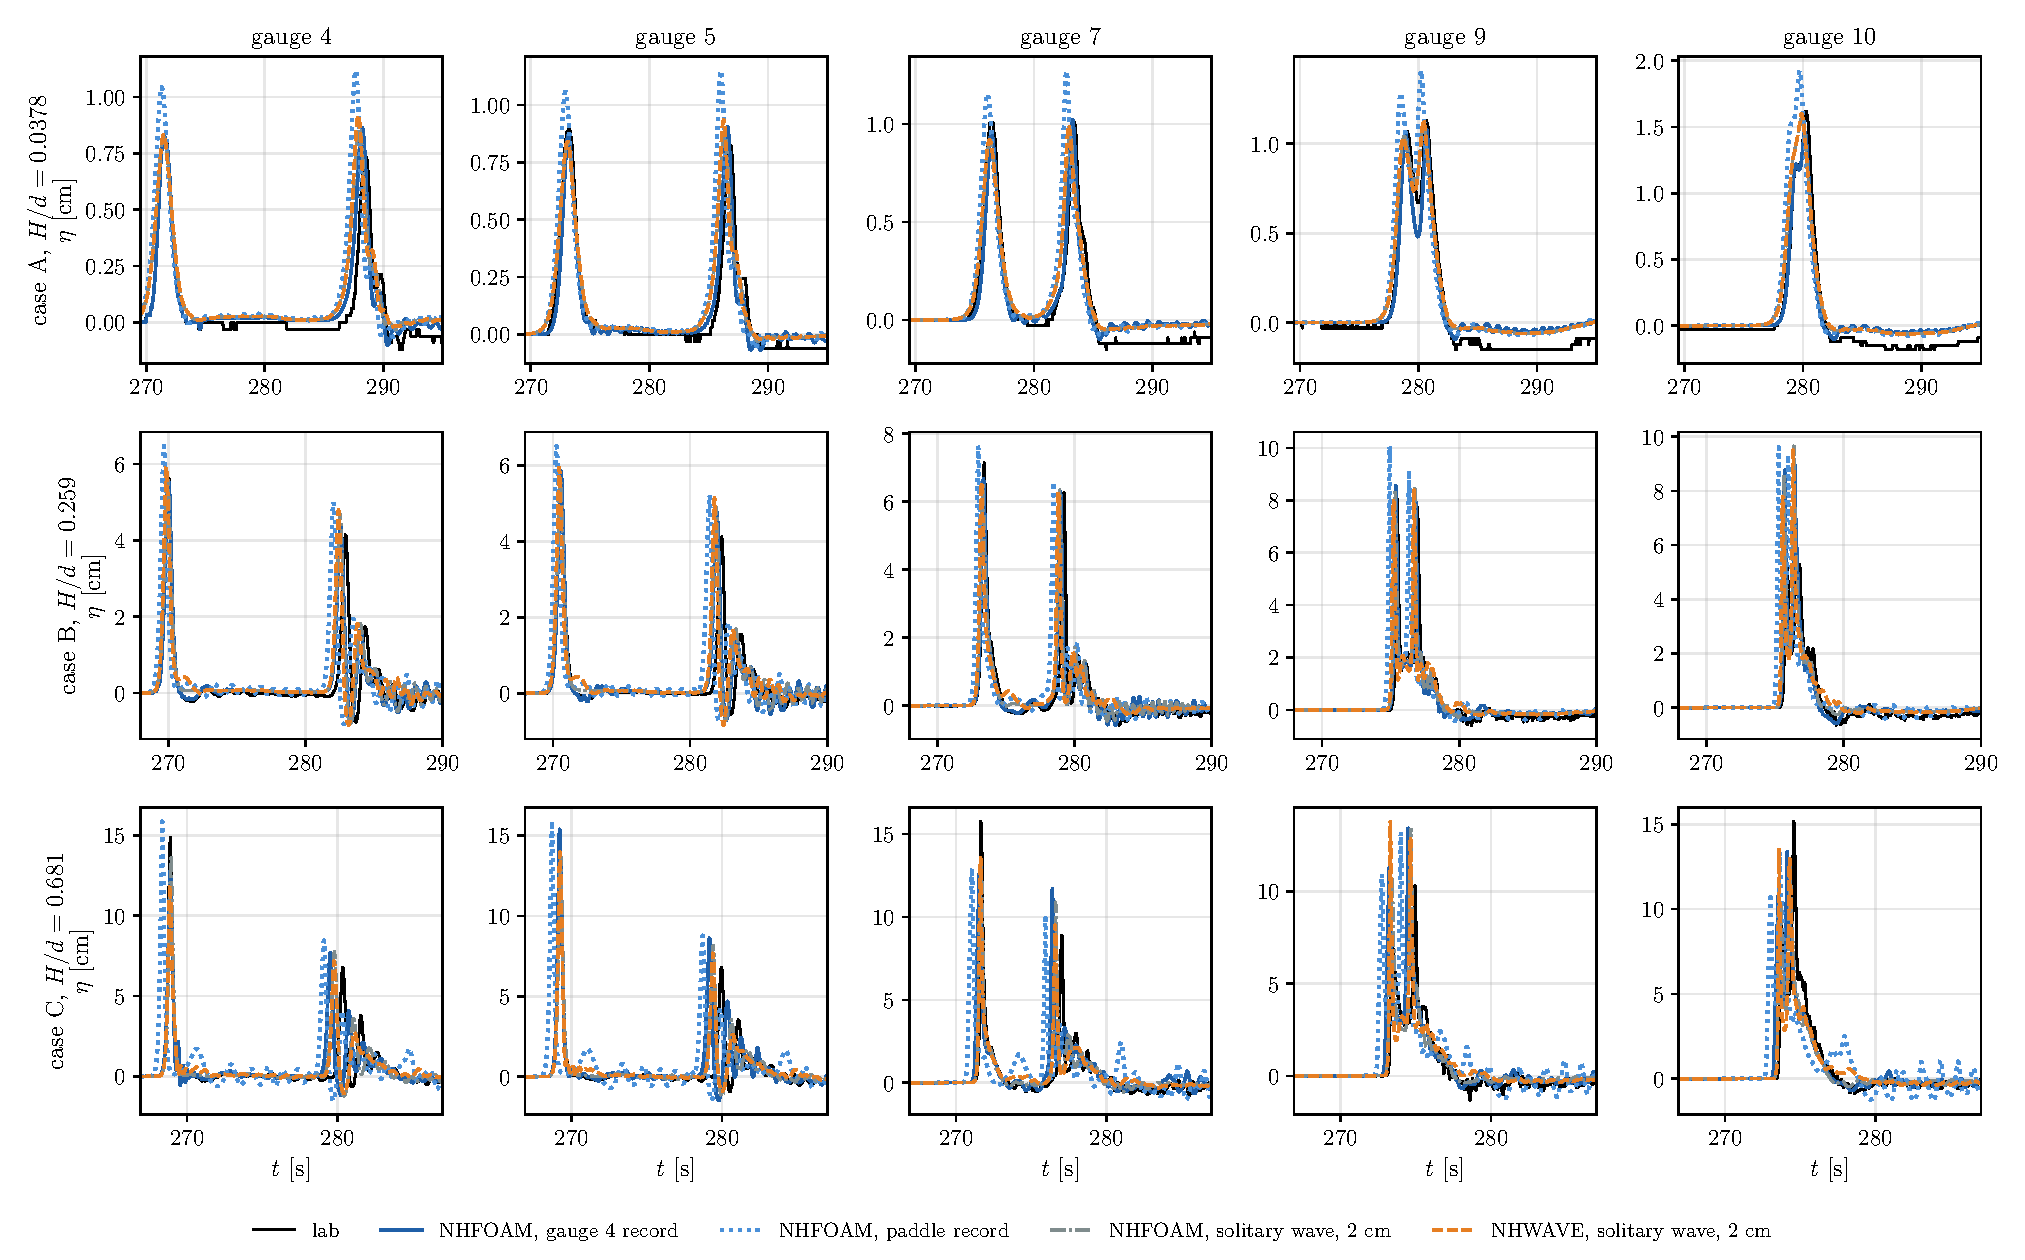
\includegraphics[width=\textwidth]{composite_beach_gauges.pdf}
\caption{Solitary waves on the composite beach, cases A--C (rows), at
gauges 4, 5, 7, 9 and 10: \NHFOAM\ driven by the record of gauge 4 and by
the paddle record (1 cm grid), \NHFOAM\ and NHWAVE (without its
$k$--$\varepsilon$ model) from the exact solitary wave (2 cm grid), against
the measurements.}
\label{fig:cb}
\end{figure}

\paragraph{The record of gauge 4} carries the measured pulse, which is not a
solitary wave: in case A it is 20\% narrower at half height than the
solitary wave of its height (1.25 s against 1.55 s). With it the incident
crests at gauges 5--8 are within 5\% of the measured ones in case A and
within 10\% in case B, they arrive within 0.13 s, and the rms difference is
the smallest of the three inputs (0.08 and 0.63 cm). The benchmark's
velocity and the celerity $\sqrt{g(d+H)}$ give the same crests within 2\% in
these cases. Case C ($H/d = 0.68$) is at the limit of the input: the
boundary column falls 14\% short of the recorded crest (22\% with
$\sqrt{g(d+H)}$), as in the flat tank at $H/h = 0.6$, and the absorption
makes up the volume, so the crest at gauge 5 is 12\% above the measured one.

\paragraph{The paddle record} makes waves 27\%, 15\% and 7\% higher than
measured at gauge 4 (cases A, B, C), which arrive 0.2--0.6 s early. In the
flat tank the paddle input reproduces the wave of a piston that follows its
record to 0.4\% up to $H/h = 0.3$, so the laboratory paddle displaced less
water than its record implies (leakage past the paddle, or the calibration
of its feedback signal; the measured heights also fell short of the target
ones). This is why the benchmark recommends the record of gauge 4.

\paragraph{Breaking.} In case C the measured wave peaks at gauge 7 (19.4 m)
and plunges before gauge 8, while the waves of both models are 14--18\%
lower at gauge 7 (\NHFOAM\ breaks at 16.8--18.4 m) and 39--75\% higher at
gauge 8: the broken waves keep too much height, as on the spilling-breaker
beaches (Section~\ref{sec:brk}).

\paragraph{\NHFOAM\ and NHWAVE} with the same input on the same grid agree
within 2\% at every gauge in case A, where the reflected crest at gauge 5 is
14\% high in NHWAVE and 8\% in \NHFOAM, and the run-up on the wall differs
by 0.03 cm. In case B NHWAVE's crests are within 6\% of \NHFOAM's. In case
C the near-limit wave loses height on the flat bed before gauge 4 in both
models, 20\% in NHWAVE and 7\% in \NHFOAM\ (which does not break there);
after that the two follow the same pattern, and NHWAVE's run-up on the wall
is the closer one (28.4 cm against 23.6 cm, measured 27.4 cm). With its
$k$--$\varepsilon$ model NHWAVE's incident crests are already 21\% low at
gauge 4 in cases B and C; its small rms in case B comes from its slower
wave, which meets the measured arrival times, not from the crests.

\paragraph{The wall and the measurements.} The run-up on the wall is 16\%
low in case A (2.30 against 2.74 cm) and 13\% low in case C (23.8 against
27.4 cm). In case B the measured 45.7 cm ($2.1d$) is a jet thrown up the
wall by the wave breaking against it, which a $\sigma$-mesh, with one free
surface per column, cannot represent; both models give 17--20 cm. Both
models also send the reflected crest back to gauges 4--7 early, by up to
0.5 s in case A, 0.2--0.5 s in B and 0.4--0.8 s in C; as they agree, the
difference probably lies in the lab (the position of the wall, or the time
the water takes to climb it and fall back). The measured crest changes by
+11\%, $-6\%$ and $-7\%$ from gauge 4 to gauge 5 on the flat bed, which a
wave of permanent form does not do: the gauges agree to about 10\%, and
their records come in steps of 0.3 mm (0.001 ft), 4\% of the crest in case
A. \NHFOAM's solitary runs on the 1 and 2 cm grids agree within 3\% at every
gauge. On one core \NHFOAM\ took 2--3 min on the 2 cm grid and NHWAVE
7--21 min, each run sharing the machine with another.

\subsection{Unstructured meshes}
\label{sec:unstr}

\NHFOAM\ takes any horizontal mesh extruded into columns. The circular basin
of Section~\ref{sec:basic} used triangles for a linear standing mode; two
tests now use them with breaking, wetting and drying, and for wave
scattering by a body (\code{validation/unstructured.py}: gmsh triangles
extruded into prisms, the points then moved onto the bathymetry).

\paragraph{Run-up on a triangulated strip.} The breaking solitary wave of
Section~\ref{sec:wd-runup} ($H/d = 0.28$, HFA, 5 mm film, no friction, 3
layers) was run on a 10 cm wide strip of Delaunay triangles with 2 cm edges
(6662 triangles, 19\,986 prisms, slip side walls) and on a strip refined
from 3 cm offshore to 1.5 cm from $x = 7$ m on (19\,083 prisms), against the
structured run of Section~\ref{sec:wd-runup} ($\Delta x = 2$ cm, one cell
wide). Until the wave reaches the beach the profiles of the three runs agree
to 0.05--0.7\% of $d$ (rms; Fig.~\ref{fig:unstr-runup}). On the triangles
the wave runs up to $R/d = 0.489$ and 0.490, against 0.531 on the
structured mesh and 0.49--0.55 in the experiments, and it gets there
3\,$t^*$ later; the backwash is slower, and at $t\sqrt{g/d} = 60$ the
shoreline of the triangles is still at $0.35\,d$ (structured $0.12\,d$).
With the upwind face depth instead of the vanLeer reconstruction
(Section~\ref{sec:wd}) the run-up on the 2 cm triangles is 0.507, while the
structured mesh gives 0.531 with either; about half of the difference
therefore comes from the TVD reconstruction of the face depth on
triangles, whose gradients are less accurate than on the regular mesh. The
backwash stays slow (0.38\,$d$ at $t\sqrt{g/d} = 60$). The cost per cell
and time step is 1.5 times that of the hexahedra.

\begin{figure}[!htbp]
\centering
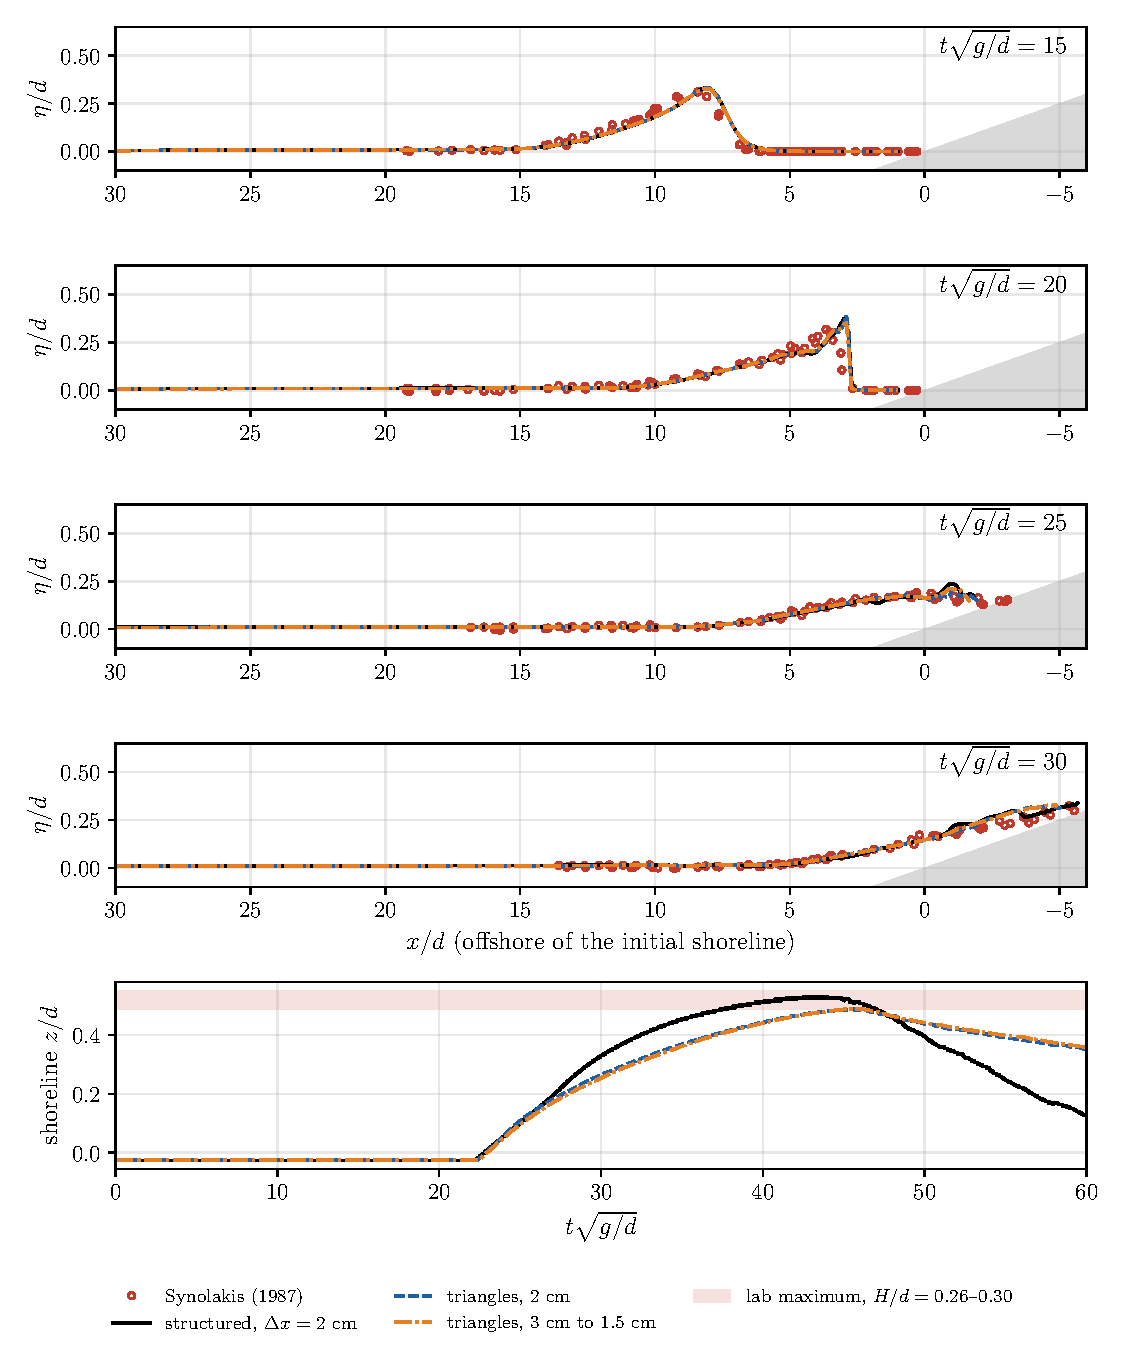
\includegraphics[width=0.85\textwidth]{unstructured_runup.pdf}
\caption{Solitary wave run-up ($H/d = 0.28$) on triangulated strips and on
the structured mesh: profiles averaged across the strip, and the shoreline
(highest wet bed) over time.}
\label{fig:unstr-runup}
\end{figure}

\paragraph{Diffraction by a vertical cylinder.} Regular waves of
$H = 1$ cm and $T = 1$ s in $h = 0.3$ m ($kh = 1.37$) from the boundary
wavemaker at $x = -3$ m meet a vertical cylinder of radius $a = 0.2$ m
($ka = 0.92$) at the origin. The half domain, 8 m by 4 m with a symmetry
wall on the axis and a 2.6 m sponge at the far end, has triangles of 2.5 cm
at the cylinder that grow to 6 cm 0.6 m away, and 4 layers (24\,289
triangles, 97\,156 prisms; Fig.~\ref{fig:cyl}a). The first-harmonic
amplitude over $t = 8$--12 s, after the waves have built up around the
cylinder and before those scattered back by the side wall and the
wavemaker return, is compared with the linear diffraction theory of
\citet{maccamy1954}. Around the cylinder the error is 0.07\,$a_I$ rms (at
most 0.095\,$a_I$); the run-up in front of it is 1.62\,$a_I$, against 1.71
(Fig.~\ref{fig:cyl}b). Along the axis in front of the cylinder the partial
standing wave has the right nodes and antinodes, the shadow behind it and
the pattern across are within a few percent of the theory, and over all 70
gauges the error is 0.06\,$a_I$ rms (Fig.~\ref{fig:cyl}c). In the window
that ends at 16 s the reflections from the walls of the half domain have
arrived (0.135\,$a_I$ rms around the cylinder). The run took 30 min on one
core for 16 s.

\begin{figure}[!htbp]
\centering
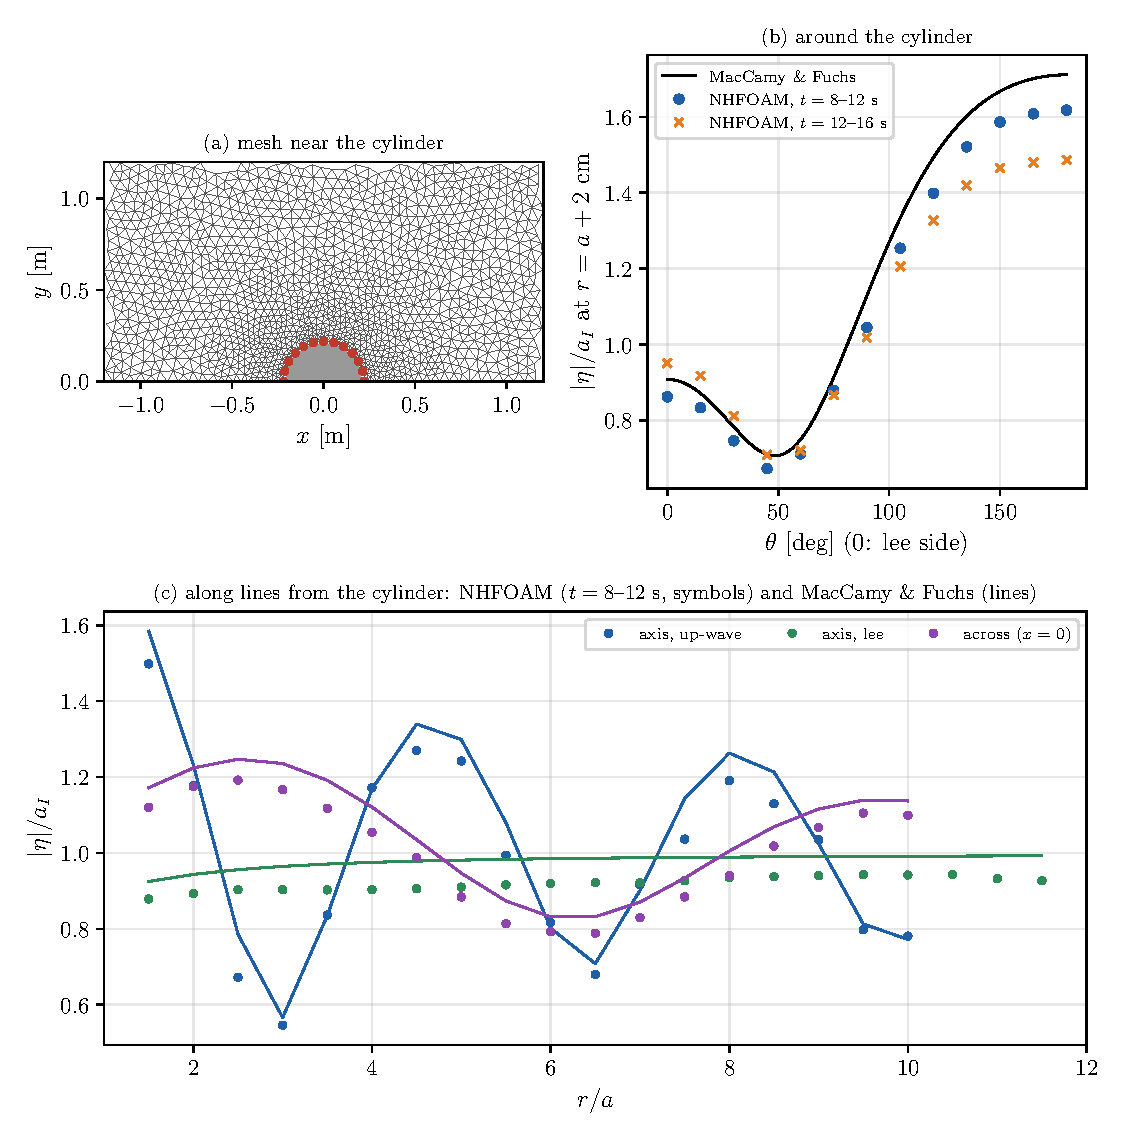
\includegraphics[width=0.78\textwidth]{cylinder_diffraction.pdf}
\caption{Diffraction by a vertical cylinder ($kh = 1.37$, $ka = 0.92$):
(a) the triangulated mesh near the cylinder and the gauges at
$r = a + 2$ cm; (b) amplitude around the cylinder; (c) amplitude along the
axis and across, against the theory of \citet{maccamy1954}.}
\label{fig:cyl}
\end{figure}

\subsection{Parallel runs, restarts and regression tests}
\label{sec:robust}
\label{sec:brk-par}

\paragraph{Breaking across processor boundaries.} A breaker that crosses a
processor boundary must be flagged as in a serial run: the flags spread
over neighbouring columns, and the persistence threshold depends on the age
of the breaking event, which travels with the wave. Ting \& Kirby's beach
with the default breaking model, run for 20 s on two processors with the
boundary at $x = 8$ m in the surf zone, now reproduces the serial run to
$4\times10^{-7}$ m at all gauges; before the ages were exchanged through the
processor patches (Section~\ref{sec:numhfa}) the difference reached 3.0 cm.
Gauges on a face between two columns are now always given to the same
column (the first one, also across processors), so that the records do not
depend on the rounding of the mesh points.

\paragraph{Restarts.} \NHFOAM\ writes its state with the fields: the time
levels of $\eta$, the face velocities of the last two levels, the surface
pressure unknowns, the breaking flags and ages, and the averaging time
(\code{uniform/NHFOAMState}). A restarted run keeps the mesh it was written
with and continues the BDF2 integration and the flux extrapolation. Ting \&
Kirby's beach (breaking, wetting and drying, averaging) restarted after 6 s
matches the continuous run to $6\times10^{-14}$ m in $\eta$ after another
6 s, and the bottom uplift to $10^{-18}$ m; without the state (Euler first
step, mesh placed on $\eta$) the differences were 2.5 mm and 4 cm/s. This
needs the fields at full precision (17 digits or binary): with 10 digits the
written state differs by $10^{-10}$, and the on/off breaking flags amplify
that to millimetres within seconds.

\paragraph{Regression suite.} \code{validation/regression.py} runs twelve short
cases in about three minutes on one core (standing and solitary waves, the
boundary wavemaker with regular and irregular waves and with measured
elevation and paddle records, a dam break and the
run-up with wetting and drying, breaking on Ting \& Kirby's beach, the
$k$--$\omega$ model, a bottom uplift and the triangulated beach) and compares
the extremes and final values of their gauge records with stored references.
It also checks that the breaking case run on two processors (with the
\code{structured} decomposition, the boundary near the breaking point) and
restarted at half time reproduces the serial, continuous run: to
$2\times10^{-7}$ m and $10^{-12}$ m.

\paragraph{Parallel speed-up.} On an otherwise idle machine with two cores
and the \code{structured} decomposition, Ting \& Kirby's beach with
breaking and wetting and drying (9200 cells, 10 s) took 102 s on one core
and 62 s on two (speed-up 1.64), and the 3D landslide tutorial (35\,280
cells, 4 s) 252 s and 131 s (1.92); the parallel runs reproduce the serial
ones to $3\times10^{-8}$ and $9\times10^{-8}$ m. The smaller 2DV case loses
more to the exchanges of the interface matrix and the breaking flags per
step.

\section{Conclusions, limitations and plans}
\label{sec:conclusions}

\NHFOAM\ follows NHWAVE's pressure arrangement on OpenFOAM's unstructured,
moving $\sigma$-meshes. The tests of \citet{ma2012} were run with both models
on the same set-ups, from the simplest upwards, and they changed the code:
\begin{itemize}[nosep]
  \item \textbf{Time accuracy.} With one outer corrector the convection term
        was linearised with the flux of the previous time level, which made the
        scheme first order in time for nonlinear waves. The convecting flux is
        now extrapolated from the last two levels. A solitary wave of
        $H/h=0.5$ lost 6.4\% of its height in 150 m before and 1.0\% after the
        fix (NHWAVE 2.3\%), at no extra cost.
  \item \textbf{Convection.} The TVD scheme damps steep short waves even when
        they do not break; filtered central differencing
        (\code{filteredLinear2V 0.2 0}) is now recommended for non-breaking
        waves. It reduced the standing-wave error to 0.16--0.25\% for
        $kD\ge 2\pi$ (NHWAVE 0.6--4.8\%) and stayed stable in 40--65 s runs over
        the submerged bar. Breaking still needs the TVD scheme.
  \item \textbf{Consistency with NHWAVE.} After the fix, the phase of the waves
        over and behind the submerged bar agrees with NHWAVE's. The closer
        match of the measured phase before the fix came from the first-order
        lag, which slowed the waves by about 0.5\%.
  \item \textbf{Resolution.} On the elliptic shoal, with twice the paper's
        grid spacing and three layers, \NHFOAM's errors at the first sections
        (0.06 and 0.13) are close to NHWAVE's on the paper's grid (0.07 and
        0.11), while NHWAVE on the coarse grid loses 30\% of the incident wave
        height before the shoal.
  \item \textbf{Robustness.} A domain in which waves break anywhere needs the
        TVD scheme and the breaking model, even outside the region of
        interest: the shoal run with the filtered scheme failed when the waves
        broke in a shallow corner, and ran on with \code{limitedLinearV} and
        the hydrostatic front approximation.
  \item \textbf{Wetting and drying.} NHWAVE's mask and thin film carry over,
        but the implicit free surface needs a limiter on the outflows (which
        keeps the volume conserved, unlike NHWAVE's clip), and the collocated
        mesh needs the upwind (TVD) depth at the side faces and the upwind
        predicted flux in supercritical flow. With the centred depth of the
        mesh faces the fronts were too slow ($R/d = 0.41$ for the solitary
        wave); with both changes the run-up is 0.531 (NHWAVE 0.512, lab
        0.49--0.55), still water stays at rest on a beach, and the
        parabolic basin is reproduced to 0.9 mm rms. A dam break on a dry
        bed showed that both models treat the film as a wet bed and follow
        Stoker's solution for it, not Ritter's. Parallel runs give the same
        run-up with a processor boundary in the swash zone (0.540 against
        0.531).
  \item \textbf{Breaking.} The HFA alone flags only the fronts of the
        bores. A persistence threshold that falls with the age of the
        breaking event and the breaking eddy viscosity of
        \citet{kennedy2000}, with horizontal mixing, nearly halve the
        surf-zone errors of the wave height on both spilling-breaker beaches (mean
        error $+6.1 \to +3.5$ cm on the beach of \citet{ting1994}, NHWAVE
        $+4.8$; rms $2.98 \to 1.54$ cm on that of \citet{hansen1979}), raise
        the set-up, and keep the measured shape of the undertow, which is
        30\% too strong (NHWAVE 60\%). Vertical mixing through the layer
        faces flattens the undertow and dissipates less. In 3D, columns
        must join a breaker at the threshold of a new breaker, or the
        breaking region creeps along oblique crests into deep water.
  \item \textbf{Longshore current.} Test 4.7 of \citet{ma2012}, in 3D
        with periodic lateral boundaries, wetting and drying, log-law
        friction and the Smagorinsky model, runs with both models on the
        same coarse grid. Both put the current at about the measured
        position (\NHFOAM: 0.265 m/s at 1.08 m from the shoreline, NHWAVE:
        0.250 m/s at 1.26 m, lab 0.39 m/s at 1.21 m) and give two thirds of
        its strength. With the HFA alone the current is 0.19 m/s and too
        close to the shoreline, as \citet{ma2012} found without turbulent
        diffusion.
  \item \textbf{Breaking parameters and closures.} Varied one at a time,
        the parameters of the default model show a shallow optimum near
        their published values: no change of $\alpha$, $\beta_F$ or
        $\delta_b$ moves the surf-zone errors by more than 8\%, and none
        removes the slow loss of height just after the breaking point.
        The kinematic onset with the crest speed estimated from the front
        face and $B_k = 0.70$ breaks at the measured place on the beach of
        \citet{ting1994}, with the smallest surf-zone error so far ($+2.4$
        cm), and 0.7 m early on that of \citet{hansen1979}. The stabilised
        $k$--$\omega$ model of \citet{larsen2018} keeps the turbulence of
        the nearly potential flow 30--60\% below that of the unstabilised
        model, but it does not replace the breaking model: without it the
        waves break 1.8 m late, and with the HFA it adds little
        dissipation.
  \item \textbf{Wave input.} The boundary wavemaker makes the target
        waves to within 0.5\%, and its active absorption keeps a closed
        flume steady (incident amplitude $1.03\,a$, against a beat between
        $0.1\,a$ and $1.1\,a$ without it); as an absorbing boundary it
        reflects 0.3--1.7\% of waves with $kh \le 1$ when given the wave's
        phase speed. Irregular JONSWAP waves keep the target spectrum,
        with $H_{m0}$ within $-4\%$ and $+2\%$ over 8 peak wavelengths.
  \item \textbf{Long runs.} The drift of the phase over the submerged bar
        (0.21 s in 20 s) came from the missing return current of the
        wave-making zone. With the return current, now the default, or the
        boundary wavemaker, the runs are steady, with an error of 1.0 cm
        in every window, and \NHFOAM's waves arrive 0.12 s early behind the
        bar crest, like those of NHWAVE and REEF3D::NHFLOW.
  \item \textbf{Unstructured meshes.} On triangulated strips the breaking
        solitary wave runs up to $R/d = 0.49$ (structured 0.531, lab
        0.49--0.55) and its backwash is slower; on a mesh refined around a
        vertical cylinder the diffracted waves are within 7\% of the theory
        of \citet{maccamy1954}.
  \item \textbf{Reproducibility.} Restarts continue the run to round-off,
        parallel runs reproduce serial ones with breakers across processor
        boundaries ($4\times10^{-7}$ m), and a regression suite of ten
        short cases checks both against stored references. The landslide
        rerun with its beach and wetting and drying showed that the wall
        was not the cause of its large trailing waves.
\end{itemize}

\paragraph{Limitations.}
\begin{itemize}[nosep]
  \item \textbf{Wetting and drying} has been tested in 2DV and on
        triangulated strips. The film acts as a wet bed, so thin swash flows
        run slower than over a truly dry bed (in NHWAVE as well), and
        puddles of a few millimetres above the film stay on the beach in
        the backwash; on triangles the run-up is 8\% lower than on the
        structured mesh and the backwash slower. A narrow cell at the
        shoreline raises the errors. It needs the interface pressure
        layout.
  \item \textbf{Breaking} has been tested on two spilling-breaker beaches
        and the longshore current. With the eddy viscosity the decay inside
        the surf zone is close to the measured one, but just after the
        breaking point the models lose too little height (3.5--4 cm too
        much at $x = 8$ m on the beach of \citet{ting1994}), and no
        parameter of the model removes this. The kinematic onset with
        $B_k \approx 0.7$--0.8 is promising but has been tested on the two
        2DV beaches only. The crest-speed estimate does not look across
        processor boundaries.
  \item \textbf{Turbulence closure.} The stabilised $k$--$\omega$ model
        gives the undertow its measured strength but, with the HFA, half
        the measured turbulent kinetic energy and little dissipation; it
        does not replace the breaking eddy viscosity.
  \item \textbf{Wave generation} is linear (no second-order correction
        for the bound long waves of wave groups). The absorbing boundary
        is uniform over the depth, so waves with $kh > 1.5$ are reflected
        by 9--13\%. Directional spreading has not been tested in a basin.
        Irregular waves lose 3--5\% of $H_{m0}$ over 12 m in the peak band,
        for a reason not yet identified.
  \item \textbf{Landslide trailing waves} are 1.5--3 times the measured ones
        (Sections~\ref{sec:seabed} and \ref{sec:ma-landslide}); the beach is
        not the cause.
  \item \textbf{OpenFOAM version.} The code was compiled and run with
        v1912 only; its API calls were checked against the v2512 headers.
\end{itemize}

\paragraph{Plans.} In order of priority:
\begin{enumerate}[nosep]
  \item breaking: the transition just after the breaking point; the
        kinematic onset ($B_k \approx 0.7$--0.8) on more beaches and on the
        longshore current, also on the grid of \citet{ma2012};
  \item second-order wave generation, and a directional-spreading test in
        a basin;
  \item the trailing waves of the landslide (slide motion, dissipation);
  \item a build and the regression suite with a current OpenFOAM release;
  \item depth-integrated granular slides for landslide tsunamis;
  \item coupling to \code{interFoam} and \code{sedInterFoam} through relaxation
        zones, and hybrid meshes around structures.
\end{enumerate}


\bibliographystyle{apalike}
\bibliography{10-References}

\appendix
\section{Building the code and setting up a case}
\label{app:usage}

\subsection{Building}

\NHFOAM\ needs the ESI OpenFOAM line (\url{https://www.openfoam.com}). It was
compiled and run with v1912, and the API calls were checked against the
v2512 headers. With the OpenFOAM environment loaded, \code{./Allwmake} builds
\begin{itemize}[nosep]
  \item \code{libNHFOAM}: the $\sigma$-column structure, mesh motion, the
        interface pressure matrix and the \code{sigmaColumn} preconditioner,
        the wave theories (linear, irregular, stream function), relaxation
        zones, seabed motion, and the boundary conditions
        \code{nhMovingSlipVelocity} and \code{nhWaveVelocity};
  \item \code{libNHFOAMturbulenceModels}: \code{kOmegaLF}, the
        stabilised $k$--$\omega$ model of \citet{larsen2018};
  \item \code{NHFOAM}: the solver;
  \item \code{nhSetWaves}: initial conditions (\code{standing},
        \code{solitary}, \code{linear}, \code{circularMode}).
\end{itemize}
\code{validation/regression.py} runs a suite of short cases against stored
references, and checks that a parallel run and a restarted run reproduce the
serial, continuous one (Section~\ref{sec:robust}).

\subsection{Mesh and fields}

The mesh must be a vertical extrusion between a top patch (\code{surface}) and
a bottom patch (\code{bottom}), with the points of each column on a vertical
line: \code{blockMesh} with vertical block edges, \code{extrudeMesh} from a 2D
mesh, or gmsh (\code{Extrude} with \code{Layers} and \code{Recombine}) followed
by \code{gmshToFoam}. The bathymetry is built into the mesh, with the top of
the mesh at the still-water level. Uniform layers are best with the interface
pressure (Section~\ref{sec:dispersion}): two layers keep the period error within
0.6\% up to $kh = 7$, three layers within 0.21\%. Periodic lateral boundaries
are pairs of \code{cyclic} patches; the fields then need their constraint
entries (\code{\#includeEtc "caseDicts/setConstraintTypes"} in
\code{boundaryField}).

\begin{table}[ht]
\centering
\caption{Boundary conditions of the fields in \code{0/}.}
\label{tab:fields}
\small
\begin{tabular}{lllp{5.2cm}}
\toprule
field & \code{surface} & \code{bottom}, walls & notes \\
\midrule
\code{U} & \code{zeroGradient} & \code{slip} or \code{noSlip} & \code{nhMovingSlipVelocity} on a moving bottom, \code{nhWaveVelocity} for a wavemaker \\
\code{p\_rgh} & \code{mixed} & \code{fixedFluxPressure} & the mixed coefficients are set by \NHFOAM \\
\code{eta} & \code{zeroGradient} & \code{zeroGradient} & one value per column \\
\bottomrule
\end{tabular}
\end{table}

\subsection{\code{constant/NHFOAMProperties}}

\begin{verbatim}
surfacePatch     surface;     // top patch
bottomPatch      bottom;      // bottom patch
minDepth         1e-4;        // smallest depth used to place mesh points
stillWaterLevel  0;           // reference for the relaxation-zone targets
pressureLocation interface;   // or cell

gauges                        // -> postProcessing/gauges/<t0>/eta.dat
{
    G1  (5.7 0 0);
}

forcingZones
{
    inlet                     // generation and absorption
    {
        type        wave;
        start       (8 0 0);  // sigma_r = 0 here ...
        end         (0 0 0);  // ... sigmaMax here
        sigmaMax    20;  exponent 2;
        waveHeight  0.02;  wavePeriod 2.02;  depth 0.4;
        direction   (1 0 0);  rampTime 4.04;
        // returnCurrent no;       // default yes (linear, irregular)
        // theory streamFunction;  waveNumber ...;  uMean ...;
        // etaCoeffs (...);  psiCoeffs (...);   from
        // validation/stream_function.py H T h [N]
        // theory irregular;  Hs 0.03;  Tp 1.5;  gamma 3.3;
        // nFrequencies 100;  seed 1;  nDirections 1;  spreading 10;
        // maxAngle 60;  periodicWidth 5.6;
        // components ((a T angle phase) ...);  // instead of JONSWAP
    }
    outlet
    {
        type        sponge;
        start       (46 0 0);  end (54 0 0);
        sigmaMax    20;
        // relaxEta false;    // damp the velocity only
    }
}

breaking
{
    model       hybrid;       // HFA | eddyViscosity | hybrid | none
    onset       etaT;         // etaT | kinematic (u_s.n > Bkin C)
    alpha       0.6;  beta 0.3;  Bkin 0.85;  crestSlope 0.01;
    persistence threshold;    // or crest (until the crest has passed)
    betaFinal   0.15; Tstar 5;   // threshold falling with the breaking age
    delta       1.2;  verticalMixing 0;     // eddy viscosity; fraction of
                                            // nu_b on the layer faces
    hydrostaticFactor 1000;
}

averaging { timeStart 95; }   // UMean, etaMean from t = 95 s

wettingDrying                 // needs pressureLocation interface
{
    minDepth         0.005;   // film of the dry columns [m]
    tolerance        1e-6;    // drying when D - minDepth <= this
    faceDepth        vanLeer; // upwind | minmod | vanLeer | MC | mesh
    faceDepthBelow   1e15;    // ... only where a column is shallower
    upwindFroude     1;       // upwind predicted flux above this (0: off)
    hydrostaticDepth 0;       // q = 0 in columns shallower than this
}

bottomFriction { Cd 0.006; }  // or { manning 0.012; } or { ks 0.0008; }

bottomMotion                  // uplift, or slide (see the source)
{
    type uplift;  min (-0.305 -1 0);  max (0.305 1 0);
    amplitude 0.0005;  history exponential;  riseTime 0.1;
}
\end{verbatim}

\subsection{Boundary wavemaker and turbulence}

A side patch makes waves (and absorbs those coming back) with
\begin{verbatim}
inlet                         // 0/U
{
    type               nhWaveVelocity;
    activeAbsorption   yes;
    absorptionCelerity shallow;   // shallow | wave | value [m/s]
    layerAverage       no;        // yes: profile averaged over each face
    wave { theory linear; waveHeight 0.041; wavePeriod 1.01; depth 0.4;
           direction (1 0 0); rampTime 2.02; }
    value              uniform (0 0 0);
}
\end{verbatim}
with \code{fixedFluxPressure} for \code{p\_rgh} and \code{zeroGradient} for
\code{eta}; \code{waveHeight 0} gives an absorbing boundary. The stabilised
$k$--$\omega$ model is selected in \code{turbulenceProperties} with
\code{simulationType RAS; RAS \{ RASModel kOmegaLF; \}} and needs the fields
\code{k}, \code{omega} and \code{nut} (wall functions on a no-slip bottom).

\subsection{Schemes and solution controls}

\begin{verbatim}
ddtSchemes { default backward 1; }        // "1": full ddt flux correction
divSchemes
{
    div(phi,U)  Gauss filteredLinear2V 0.2 0;  // non-breaking waves
//  div(phi,U)  Gauss limitedLinearV 1;        // with breaking (bores)
}

PIMPLE
{
    nOuterCorrectors          1;
    nCorrectors               3;
    nNonOrthogonalCorrectors  1;     // over sloping beds
    fluxExtrapolation         true;  // default with backward
}

p_rgh
{
    solver          PCG;
    preconditioner  sigmaColumn;     // DIC in the cell layout
    tolerance       1e-10;
    relTol          0.01;
}
\end{verbatim}

Without the ddt coefficient OpenFOAM limits its ddt flux correction, and waves
are visibly damped; \NHFOAM\ warns if it is missing. In the interface layout
only PCG and PBiCGStab are used, and any preconditioner other than
\code{diagonal} or \code{none} is replaced by \code{sigmaColumn}. The unknowns
are written as \code{pI}, the pressure on the bottom interface of each cell.

The time step should resolve the shortest wave that matters, not only the
peak period: behind the submerged bar the free higher harmonics have periods
of $T/2$ and $T/3$ (Section~\ref{sec:bar10}).

\subsection{Initial conditions and parallel runs}

Initial conditions are set with \code{nhSetWaves}
(\code{system/nhSetWavesDict}); \NHFOAM\ moves the mesh onto the initial
$\eta$ at start-up. Whole columns must stay on one processor, so the
decomposition uses the \code{structured} method on the bottom patch:
\begin{verbatim}
method structured;
structuredCoeffs
{
    method  simple;
    patches (bottom);
    simpleCoeffs { n (2 1 1); }
}
\end{verbatim}

\subsection{Tutorials and validation scripts}

The tutorials are \code{standingWave}, \code{solitaryWave},
\code{submergedBar}, \code{circularBasin} (3D unstructured prisms),
\code{bottomUplift}, \code{landslide3D}, \code{breakingSlope},
\code{beachRunup} (the solitary wave of Section~\ref{sec:wd-runup}, with
wetting and drying), \code{longshoreCurrent} (Section~\ref{sec:brk-ls}) and
\code{irregularWaves} (JONSWAP waves from the boundary wavemaker, an absorbing
boundary at the other end, no relaxation zones). Each runs with
\code{./Allrun}. The folder \code{validation/} holds the scripts that build
the validation cases and make the figures of this report:
\begin{itemize}[nosep]
  \item \code{make\_case.py}, \code{ma2012.py}: the cases of
        Sections~\ref{sec:verification} and~\ref{sec:ma2012};
  \item \code{wetdry.py}, \code{longshore.py}: wetting and drying, breaking
        and the longshore current;
  \item \code{wavemaker.py}, \code{unstructured.py}: the tests of
        Section~\ref{sec:ext} (the latter with gmsh);
  \item \code{other\_models.py}: the input of NHWAVE and REEF3D::NHFLOW;
  \item \code{stream\_function.py}: the coefficients of nonlinear waves;
  \item \code{regression.py}: the regression suite;
  \item \code{make\_figures.sh}: the figures.
\end{itemize}


\end{document}
